
\begin{figure}[ht]
	\begin{minipage}{0.2\textwidth}
		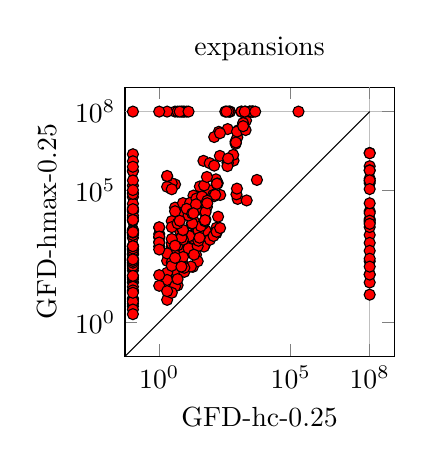
\begin{tikzpicture}
\begin{axis}[extra x tick style={grid=major}, extra x ticks=100000000, extra y tick style={grid=major}, extra y ticks=100000000, height=5cm, legend cell align=left, legend style={at=(1.3, 0.5)}, title=expansions, width=5cm, xlabel=GFD-hc-0.25, xmin=0.05, xmode=log, ylabel=GFD-hmax-0.25, ymin=0.05, ymode=log]
\addplot[color=red, mark=*, mark options={{draw=black}}, only marks] coordinates {
(0.100000, 2971) (14, 1892) (100000000, 840413) (0.100000, 2446) (58, 3037) (100000000, 2688956) (3, 706) (48, 1342391) (0.100000, 811) (4, 170892) (100000000, 65) (208, 67738) (0.100000, 21631) (0.100000, 730) (668, 1368076) (19, 1534) (100000000, 2048) (1019, 19611126) (0.100000, 32) (100000000, 2617617) (18, 1954) (55, 892) (3558, 100000000) (2, 213) (494, 100000000) (9, 496) (25, 364) (4, 22448) (0.100000, 2397766) (13, 636) (649, 2261740) (9, 1572) (0.100000, 4) (8, 33393) (819, 6917972) (958, 47992) (0.100000, 1591) (480, 100000000) (1, 2242) (0.100000, 245) (0.100000, 58) (0.100000, 256) (20, 64248) (0.100000, 553753) (0.100000, 16051) (100000000, 4096) (0.100000, 187) (1, 3844) (0.100000, 166) (1332, 100000000) (0.100000, 2506) (149, 2378) (100000000, 192711) (2768, 100000000) (100000000, 8192) (1, 1108) (3, 344) (1997, 45935775) (14, 1861) (863, 71716) (0.100000, 2323) (196523, 100000000) (0.100000, 56875) (4, 1109) (1908, 100000000) (5, 826) (1, 745) (164, 198133) (0.100000, 19141) (0.100000, 154345) (100000000, 283576) (0.100000, 17761) (0.100000, 3286) (9, 109) (0.100000, 217) (0.100000, 14) (2684, 100000000) (0.100000, 219) (50, 5809) (43, 36387) (0.100000, 745) (0.100000, 9131) (0.100000, 16896) (6, 12007) (9, 100000000) (17, 5356) (31, 3001) (100000000, 587761) (4, 1108) (15, 34032) (0.100000, 226) (0.100000, 379) (8, 152) (0.100000, 11285) (78, 104720) (6, 3101) (45, 5283) (0.100000, 548746) (50, 741) (0.100000, 772) (1563, 28711853) (21, 6526) (40, 18270) (25, 19579) (100000000, 232531) (100000000, 16384) (100000000, 580396) (426, 100000000) (0.100000, 33) (5, 73) (1, 4035) (65, 23798) (11, 100000000) (29, 764) (4, 347) (395, 1143601) (0.100000, 5) (0.100000, 586) (0.100000, 7615) (85, 1355) (801, 7341225) (0.100000, 8) (19, 126) (931, 10420707) (2, 7) (0.100000, 246) (35, 142466) (2109, 42030) (26, 49620) (83, 1096038) (2, 50) (3, 188791) (112, 67588) (0.100000, 370) (2, 138858) (3, 112017) (38, 4427) (29, 205) (9, 81) (100000000, 13979) (151, 3851) (7, 100000000) (0.100000, 7) (8, 1360) (100000000, 1024) (3, 962) (4, 100000000) (3, 6886) (116, 1880) (51, 156560) (409, 1131640) (8, 100000000) (400, 21653693) (902, 118208) (5, 100000000) (3, 21) (0.100000, 43) (4, 1241) (100000000, 32) (123, 884552) (3510, 100000000) (0.100000, 151) (0.100000, 2566) (2841, 100000000) (3709, 100000000) (0.100000, 2056) (2, 19) (0.100000, 559) (0.100000, 15) (803, 5975018) (100000000, 6272) (1, 1627) (2, 75) (0.100000, 50) (907, 17460317) (8, 297) (18, 5647) (122, 60875) (5183, 252962) (7, 1627) (31, 1236) (8, 3101) (184, 17075893) (0.100000, 7036) (42, 59583) (0.100000, 22) (0.100000, 91) (155, 185045) (6, 100000000) (824, 6722843) (0.100000, 3076) (3, 1438) (0.100000, 113) (0.100000, 31561) (13, 11292) (8, 3160) (100000000, 7138) (0.100000, 19591) (4, 803) (1920, 19918398) (0.100000, 136) (2, 346276) (0.100000, 407) (0.100000, 100000000) (151, 2707) (3, 4066) (2, 357856) (100000000, 244221) (2, 40) (143, 266816) (57, 8012) (100000000, 205) (16, 129) (0.100000, 6) (11, 20161) (1, 1780) (100000000, 64) (0.100000, 1294345) (135, 69035) (5, 5617) (54, 6870) (4, 16278) (100000000, 113756) (0.100000, 181) (3249, 100000000) (58, 15290) (0.100000, 2521) (65, 328078) (100000000, 512) (166, 185292) (100000000, 32768) (0.100000, 16) (0.100000, 241546) (1334, 100000000) (1, 1053) (0.100000, 3) (0.100000, 507) (3, 187) (391, 846921) (6, 7076) (100000000, 5412) (325, 100000000) (2, 100000000) (9, 116) (0.100000, 802036) (0.100000, 57) (3, 138) (55, 7441) (1776, 100000000) (0.100000, 2791) (67, 40955) (0.100000, 211) (5, 25) (4, 23) (4451, 100000000) (156, 182080) (0.100000, 7625) (2, 406) (34, 1614) (0.100000, 2626) (13, 100000000) (18, 13376) (1, 24) (1542, 36749162) (123, 10801620) (100000000, 256) (3, 13) (204, 15117895) (0.100000, 632) (173, 10156) (0.100000, 241) (1, 61) (25, 29955) (202, 2073240) (7, 128) (100000000, 11) (4, 276) (0.100000, 80806) (100000000, 128) (416, 1656947) (5, 43) (0.100000, 13) (0.100000, 2) (67, 32916) (0.100000, 74443) (0.100000, 766) (206, 3759) (1, 100000000) (21, 365) (2, 15) (1, 573) (20, 13650) (362, 100000000) (0.100000, 104311) (1545, 27889713)
};
\addplot[color=black] coordinates {(0.050000, 0.050000) (100000000, 100000000)};
\end{axis}
\end{tikzpicture}
	\end{minipage}
	\hfill
	\begin{minipage}{0.2\textwidth}
		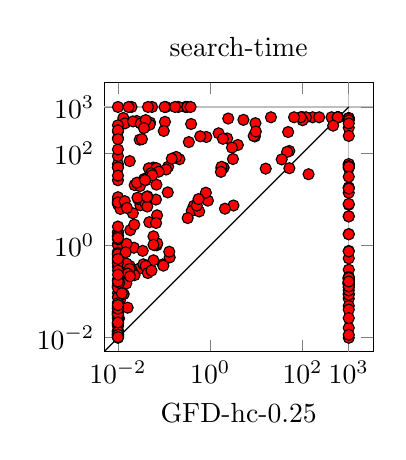
\begin{tikzpicture}
\begin{axis}[extra x tick style={grid=major}, extra x ticks=1000, extra y tick style={grid=major}, extra y ticks=1000, height=5cm, legend cell align=left, legend style={at=(1.3, 0.5)}, title=search-time, width=5cm, xlabel=GFD-hc-0.25, xmin=0.005, xmode=log, ymin=0.005, ymode=log]
\addplot[color=red, mark=*, mark options={{draw=black}}, only marks] coordinates {
(0.028531, 0.314060) (0.010000, 0.141879) (0.069130, 1.009340) (0.214463, 73.840300) (1000, 47.512000) (1000, 18.145400) (164.948000, 598.097963) (0.010000, 0.020384) (0.888732, 9.357150) (0.010000, 0.010339) (0.010547, 0.026249) (0.010000, 9.696930) (1.949160, 48.497200) (0.010114, 0.348226) (0.035558, 0.390635) (0.030658, 7.416310) (0.020102, 0.282966) (0.093627, 0.389600) (1000, 0.146346) (0.010000, 0.037258) (0.047734, 3.195270) (0.054777, 1000) (0.010000, 0.018990) (0.010000, 0.027059) (0.010000, 291.270000) (1000, 0.070376) (1000, 569.424419) (1000, 0.147251) (0.010000, 0.011000) (0.010000, 0.014282) (0.010000, 0.032966) (9.261430, 229.940000) (1000, 13.833200) (568.991588, 598.365640) (1000, 56.506600) (0.010000, 0.093661) (0.010000, 0.625783) (0.010000, 212.797000) (1000, 57.913900) (585.815451, 599.292347) (0.018514, 2.145660) (0.030658, 23.419100) (0.058698, 0.476285) (0.010000, 0.124818) (0.039912, 0.360602) (1000, 0.298156) (0.010000, 0.032660) (0.010000, 0.441437) (0.441380, 7.235470) (1000, 52.462000) (1000, 0.526094) (0.010000, 0.739707) (0.109002, 1000) (0.010000, 0.128580) (0.010000, 0.533941) (0.044337, 0.253154) (8.732200, 236.280000) (0.821598, 223.901000) (0.010000, 0.349141) (0.010000, 0.415298) (0.010000, 0.012020) (51.444700, 111.268000) (1000, 0.200383) (1000, 0.155744) (1000, 0.122064) (0.010000, 0.125091) (0.010000, 0.654800) (0.058423, 48.598600) (0.017100, 0.215000) (0.018001, 67.173300) (0.049603, 459.697721) (0.010000, 1000) (0.062464, 1.013790) (0.070845, 1.111720) (0.022982, 20.293900) (0.010000, 0.010941) (0.010000, 0.010000) (0.010000, 1.087460) (0.010000, 57.810300) (1000, 0.149782) (1000, 0.089930) (0.010000, 0.047572) (1000, 0.188603) (0.010000, 1.914130) (1000, 0.161828) (0.010000, 1.004810) (0.027428, 10.144400) (1000, 0.085536) (0.010000, 0.691930) (0.289593, 1000) (0.070357, 4.489520) (1000, 550.260712) (2.323220, 208.309000) (1000, 578.774518) (228.567000, 598.501116) (1000, 560.307000) (1.744380, 46.789000) (0.017942, 0.359657) (0.017776, 0.221800) (0.010000, 8.325430) (0.037782, 27.362300) (0.802361, 13.916800) (0.384356, 427.486000) (0.104265, 475.926000) (0.010000, 0.011866) (0.010930, 0.047907) (0.010000, 0.662245) (0.013085, 576.713000) (0.010000, 0.020199) (0.010000, 0.560587) (0.010000, 48.464000) (0.015242, 0.407146) (1000, 17.712200) (0.122342, 50.788600) (94.658300, 598.357417) (0.010000, 0.031758) (0.046649, 46.875400) (3.955460, 150.179000) (0.010000, 8.375120) (1.745930, 50.451300) (0.010381, 0.663351) (0.096368, 0.365264) (0.010000, 0.021505) (0.010000, 0.031001) (0.010000, 8.778260) (0.010000, 0.644579) (1000, 0.048968) (0.058784, 1.575660) (0.011130, 0.065548) (0.021027, 4.983350) (9.504350, 445.596445) (423.753000, 597.979372) (1000, 0.208494) (0.010000, 7.778180) (1.700400, 39.241200) (0.010000, 0.020862) (0.068110, 20.766900) (0.010000, 0.498735) (0.010000, 0.012132) (0.019643, 1000) (0.025550, 495.998221) (46.195600, 106.286177) (1000, 355.522000) (0.203845, 1000) (0.010000, 0.017955) (580.252808, 597.421969) (0.010000, 0.033312) (0.010000, 0.035483) (1000, 0.157770) (0.011288, 6.192890) (0.098322, 302.164000) (0.039069, 8.381740) (0.397300, 5.635290) (0.053284, 0.285385) (0.010000, 0.057473) (100.975000, 598.216867) (0.010000, 0.025870) (1000, 0.195165) (0.010000, 0.010978) (0.010000, 1.975790) (0.010000, 0.043581) (0.172095, 1000) (0.010000, 1.590360) (15.893100, 46.122117) (1000, 4.261360) (1000, 1.757520) (580.598600, 594.655141) (1000, 7.611890) (0.016215, 0.044811) (0.043216, 6.965240) (0.014153, 441.236015) (0.013324, 0.088213) (0.067668, 47.186100) (0.010000, 0.185382) (0.010000, 0.076204) (584.028800, 596.980998) (1000, 0.016357) (0.010000, 11.088200) (0.039464, 25.813500) (0.021167, 486.462518) (1000, 511.635237) (0.048727, 413.388000) (1000, 0.760297) (0.182816, 82.580300) (0.010000, 0.074801) (20.621400, 598.119890) (0.022172, 0.892949) (0.015340, 1.087410) (0.132199, 0.551221) (0.010000, 8.553830) (0.066446, 9.857860) (0.022853, 0.227104) (0.014732, 0.711961) (0.010000, 0.013969) (0.044813, 1000) (5.221790, 525.968498) (0.016285, 0.207687) (0.036913, 27.439100) (35.287900, 73.143364) (0.029990, 19.276300) (0.029580, 195.461000) (0.010000, 0.035689) (0.010000, 0.133593) (0.010000, 25.876100) (0.110527, 44.192400) (0.102309, 1000) (0.010000, 0.056058) (118.557000, 597.986894) (0.010000, 0.013781) (0.025675, 22.855600) (100.015000, 516.268905) (0.010000, 400.294000) (0.010000, 0.044326) (0.010000, 0.027529) (0.016945, 1000) (1000, 17.061700) (593.707266, 595.013936) (0.010000, 0.414810) (2.951390, 131.703000) (1000, 7.956260) (3.176630, 7.332720) (0.076434, 39.598700) (1000, 0.010000) (1.516048, 269.118000) (0.010000, 1.627680) (3.097730, 74.544600) (0.031105, 437.880117) (0.010000, 0.043703) (0.010000, 0.049372) (0.013997, 9.101260) (1000, 4.270620) (0.040016, 519.573000) (0.052631, 36.732000) (0.010000, 0.010387) (0.017830, 0.310687) (0.010000, 1.576880) (0.010000, 0.120594) (0.010000, 1.353550) (0.010000, 0.030457) (0.043659, 11.569400) (1000, 50.341200) (0.010000, 86.735000) (1000, 0.178393) (0.010000, 119.999000) (0.010000, 0.013099) (0.010000, 0.018442) (1000, 0.740091) (0.317699, 1000) (0.016285, 0.246044) (0.010000, 0.011925) (91.138600, 598.361146) (0.146924, 75.848100) (0.575185, 5.450780) (0.010000, 49.201700) (1000, 0.106344) (1000, 0.153929) (0.010000, 0.036721) (0.012169, 0.091736) (0.509863, 7.281820) (48.657400, 286.284000) (65.293700, 598.130903) (0.010000, 32.505000) (0.058824, 1.032870) (2.447110, 562.072608) (0.010000, 2.568680) (0.342952, 173.454000) (0.010000, 0.032530) (0.010000, 0.013371) (0.015131, 0.149984) (2.080980, 6.257675) (0.120053, 14.097800) (0.010000, 1.456300) (0.605574, 231.769000) (0.026458, 10.813300) (0.036528, 348.712000) (0.010651, 0.155582) (0.010000, 0.173754) (0.034320, 0.764386) (1000, 439.919507) (0.010000, 0.287413) (9.697540, 293.971000) (1.879740, 204.617000) (0.015641, 6.487840) (51.669200, 47.105461) (1000, 0.143147) (0.010000, 0.013457) (1000, 0.040705) (581.975225, 598.321136) (1000, 0.195246) (1000, 0.158616) (1000, 0.197603) (0.042501, 11.368500) (0.556439, 10.099300) (0.010000, 0.011628) (0.010000, 0.510173) (0.018328, 0.213925) (573.652052, 596.079760) (1000, 0.026707) (575.292850, 597.331070) (0.022572, 2.822820) (0.324084, 3.919240) (0.010000, 0.042692) (1000, 0.129543) (0.010000, 0.011598) (0.374536, 1000) (0.010000, 312.369000) (1000, 0.011587) (0.010000, 0.050968) (0.129126, 0.730525) (1000, 235.834000) (0.067089, 3.069910) (0.055317, 33.004900) (0.010000, 0.166198) (0.033064, 200.660000) (134.652364, 34.887698) (1000, 30.773200) (0.010000, 0.010325) (458.991556, 394.041305) (0.010000, 201.330000) (0.010000, 0.021533) (1000, 0.165509) (1000, 1.747380) (0.010032, 0.233055) (0.038649, 26.114200)
};
\addplot[color=black] coordinates {(0.0050000, 0.0050000) (1000, 1000)};
\end{axis}
\end{tikzpicture}
	\end{minipage}


	\begin{minipage}{0.2\textwidth}
		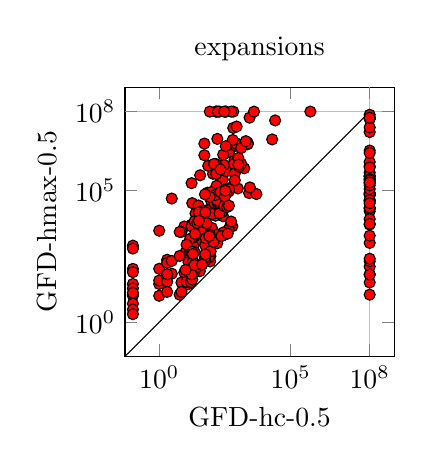
\begin{tikzpicture}
\begin{axis}[extra x tick style={grid=major}, extra x ticks=100000000, extra y tick style={grid=major}, extra y ticks=100000000, height=5cm, legend cell align=left, legend style={at=(1.3, 0.5)}, title=expansions, width=5cm, xlabel=GFD-hc-0.5, xmin=0.05, xmode=log, ylabel=GFD-hmax-0.5, ymin=0.05, ymode=log]
\addplot[color=red, mark=*, mark options={{draw=black}}, only marks] coordinates {
(652, 23964757) (194, 100000000) (28, 1247) (147, 100000000) (100000000, 11) (100000000, 840413) (326, 100000000) (100000000, 16702396) (179, 14491) (68, 82576) (100000000, 65) (602, 4359) (24, 13367) (59, 264) (3, 69) (259, 263094) (100000000, 270832) (417, 25540) (54, 1966) (63, 17624) (1, 28) (100000000, 128) (100000000, 205) (88, 319) (20, 198) (10, 447) (729, 1451467) (93, 41213) (2, 233) (100000000, 1024) (386, 92308) (1025, 997124) (521, 5111) (100000000, 20981) (1, 10) (100000000, 52302447) (144, 100000000) (347, 2631585) (649, 4842364) (70, 2924) (1, 106) (100000000, 192711) (137, 11063) (155, 36643) (150, 36643) (86, 202) (803, 6434752) (12, 39) (151, 150205) (18, 89) (52, 6085027) (145, 36643) (1, 38) (2, 49) (36, 380600) (460, 115325) (266, 10562) (78, 1815) (17, 5009) (0.100000, 10) (52, 2196973) (100000000, 74322) (349, 100000000) (443, 2938657) (100000000, 38907) (12, 27) (100000000, 32) (269, 2318245) (223, 817242) (77, 284) (187, 14177) (432, 3279) (20, 776) (0.100000, 105) (126, 34084) (100, 3806) (100000000, 81330) (2614, 80074) (100000000, 3309201) (727, 450815) (78, 1060) (111, 433598) (0.100000, 11) (100000000, 65313) (9, 77) (100000000, 16384) (493, 125022) (159, 36643) (0.100000, 28) (974, 119944) (443, 91606) (24, 98) (17, 4715) (18, 33187) (35, 86) (1233, 932069) (6, 11) (100000000, 482812) (100000000, 1222697) (9, 4284) (1, 2984) (0.100000, 5) (20, 147) (543, 6627) (19675, 8761602) (31, 27029) (21, 76) (105, 12812) (449, 111835) (23, 147) (160, 987) (92, 86481) (29, 6515) (7, 32) (23, 5902) (2282, 6685177) (56, 836) (100000000, 59040002) (242, 15037) (84, 100000000) (22, 1800) (354, 77219) (793, 5077544) (652, 100000000) (7, 2696) (30, 137) (158, 42285) (6, 2675) (100000000, 42073) (2, 179) (33, 6745) (195, 13504) (18, 1573) (100000000, 348502) (75, 1846) (40, 2772) (164, 2125) (162, 9193600) (100000000, 337294) (147, 427926) (2, 34) (172, 100000000) (2726, 58800144) (678, 1023342) (133, 67358) (13, 230) (100000000, 1919) (100000000, 72844) (272, 1989) (100000000, 205227) (296, 25836) (11, 34) (4008, 100000000) (277, 2558) (352, 540153) (46, 16621) (82, 1846) (56, 225) (7, 14) (289, 933590) (55, 282) (17, 4295) (63, 5710) (100000000, 113756) (16, 33) (13, 190) (0.100000, 747) (90, 490) (2, 14) (27, 124) (100000000, 75797336) (22, 6819) (100000000, 58708639) (213, 87835) (0.100000, 19) (17, 190693) (28, 5833) (100000000, 5058) (0.100000, 807) (2228, 5730375) (83, 57753) (100000000, 20595) (100000000, 64) (100000000, 364225) (19, 202) (56, 378) (310, 59125) (32, 14940) (84, 2100) (18, 41) (1707, 700030) (115, 1104) (15, 520) (737, 444814) (17, 65) (22, 464) (22, 147) (551, 100000000) (100000000, 43567) (146, 1007174) (2159, 5841704) (3, 211) (15, 1458) (1069, 811635) (295, 100000000) (10, 96) (1302, 1048225) (100000000, 270540) (0.100000, 3) (381, 23581) (100000000, 244805) (57, 14941) (43, 153) (2352, 6018469) (3, 49622) (0.100000, 622) (835, 6074570) (25480, 46273952) (59, 1526) (1017, 1730892) (100000000, 22374) (100000000, 755522) (2, 66) (73, 865105) (446, 26597) (100000000, 256) (231, 1852) (625, 8328784) (340, 4845380) (11, 876) (100000000, 8192) (100000000, 2688956) (100000000, 157425) (100000000, 25106283) (100000000, 201980) (100000000, 57729847) (323, 98315) (100000000, 33063) (80, 1846) (401, 2296) (100000000, 5412) (745, 243614) (121, 1023724) (4955, 73726) (18, 474) (876, 27067605) (1304, 4123680) (6, 327) (55, 71498) (0.100000, 79) (32, 7110) (212, 635569) (23, 2237) (0.100000, 13) (19, 386) (0.100000, 2) (1960, 7525022) (556807, 100000000) (1028, 965313) (2800, 131570)
};
\addplot[color=black] coordinates {(0.050000, 0.050000) (100000000, 100000000)};
\end{axis}
\end{tikzpicture}
	\end{minipage}
	\hfill
	\begin{minipage}{0.2\textwidth}
		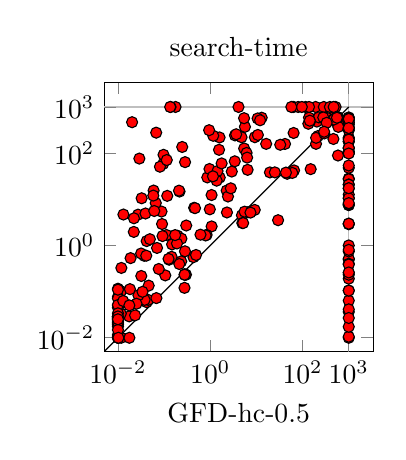
\begin{tikzpicture}
\begin{axis}[extra x tick style={grid=major}, extra x ticks=1000, extra y tick style={grid=major}, extra y ticks=1000, height=5cm, legend cell align=left, legend style={at=(1.3, 0.5)}, title=search-time, width=5cm, xlabel=GFD-hc-0.5, xmin=0.005, xmode=log, ymin=0.005, ymode=log]
\addplot[color=red, mark=*, mark options={{draw=black}}, only marks] coordinates {
(0.041854, 0.058998) (0.017512, 0.029074) (583.951830, 578.087266) (0.037065, 0.597193) (0.011856, 0.325930) (562.098282, 570.258813) (0.234970, 0.452103) (0.095245, 58.273000) (4.848530, 4.508220) (0.010000, 0.019311) (0.861978, 29.773200) (65.362500, 42.249900) (1000, 212.089324) (0.013125, 4.676810) (466.213000, 593.853868) (0.031718, 0.669523) (0.246724, 135.894000) (0.010000, 0.028847) (0.045140, 0.066215) (578.217781, 569.525860) (0.037833, 0.066226) (0.215847, 14.712000) (1.601492, 29.499500) (191.180600, 1000) (6.540580, 5.245030) (0.010000, 0.010042) (1000, 413.468000) (1000, 28.137200) (63.917500, 1000) (116.044900, 1000) (195.385000, 158.980346) (0.010000, 0.027245) (137.798000, 588.061800) (0.449681, 0.586254) (2.923400, 39.887900) (1000, 27.132800) (1000, 178.287123) (0.097101, 91.953100) (0.010000, 0.017650) (1.066810, 12.365600) (1.069230, 2.583420) (0.010000, 0.024115) (0.196374, 1.618480) (0.027724, 0.083583) (0.106003, 0.224642) (589.323401, 424.172000) (0.276432, 0.120557) (137.913000, 1000) (0.018779, 0.531310) (298.563300, 565.755300) (586.411735, 501.082590) (215.539000, 234.637000) (0.176659, 1000) (0.070280, 0.882896) (0.137911, 1000) (1000, 455.694400) (0.011648, 0.102102) (5.522910, 5.392900) (1000, 0.190798) (1000, 0.010000) (2.265700, 15.438200) (331.121500, 584.845830) (0.010000, 0.021178) (0.010000, 0.026272) (567.056913, 584.249175) (571.506110, 593.732757) (1000, 0.010558) (574.517335, 564.899979) (287.868000, 1000) (0.301398, 2.703370) (0.284444, 63.782600) (0.010000, 0.010000) (0.961149, 45.271200) (0.010000, 0.051108) (1000, 100.360018) (0.281107, 0.230384) (462.047500, 536.881400) (1000, 100.205057) (1.590130, 218.728000) (521.481018, 566.063397) (203.939000, 482.329000) (0.032044, 0.217965) (1000, 512.057896) (1000, 0.063750) (0.010000, 0.010808) (1000, 0.036456) (0.210360, 15.388900) (1000, 568.279600) (1000, 107.623000) (1000, 593.717716) (0.158121, 1.608910) (1000, 20.903804) (0.297253, 0.232706) (1000, 354.828228) (259.726990, 593.197490) (478.359803, 1000) (2.297260, 5.185390) (0.010000, 0.025250) (579.021152, 593.814848) (59.386504, 1000) (0.027262, 4.648260) (19.599300, 38.239400) (0.447559, 6.548910) (1000, 10.593297) (1000, 0.493199) (1000, 7.462530) (41.617210, 158.059000) (1000, 0.105815) (46.388700, 35.714100) (592.167364, 591.707802) (1000, 2.968010) (553.195883, 578.374876) (1000, 103.731000) (0.237001, 1.405810) (0.010000, 0.028545) (223.793300, 595.052587) (537.874753, 562.740729) (9.247950, 221.428000) (0.018215, 0.113035) (1000, 1.000170) (1000, 0.256493) (1000, 0.017302) (1000, 573.958000) (1000, 0.232753) (0.148965, 1.054250) (196.353000, 214.566000) (584.748496, 88.786300) (0.041061, 0.600610) (1000, 214.752031) (0.832867, 1.691500) (0.010000, 0.076989) (2.418060, 11.496100) (0.087744, 5.424880) (5.633600, 371.417000) (595.752315, 591.951122) (0.010000, 0.071111) (1.374770, 25.320300) (9.179850, 5.884340) (1000, 48.045600) (583.857618, 408.846000) (465.185676, 202.442000) (80.251000, 1000) (1000, 0.516748) (0.112633, 1.681790) (1.548280, 117.954000) (1000, 20.741555) (0.010000, 0.026762) (582.970766, 541.620603) (280.171700, 593.289740) (145.512000, 491.027000) (96.254700, 1000) (4.945770, 3.053140) (1000, 0.401467) (10.741100, 247.753000) (0.010000, 0.011544) (1000, 7.587580) (0.081195, 50.735000) (1000, 464.929000) (0.010000, 0.028895) (556.176868, 587.599603) (0.011523, 0.033378) (1000, 128.040106) (0.065914, 8.298160) (3.429660, 242.416000) (1000, 0.104959) (0.059249, 15.471600) (25.077300, 38.284300) (0.039527, 4.927230) (0.128162, 0.491366) (0.793168, 1.645930) (552.808508, 582.840500) (1000, 177.756549) (12.993800, 585.597000) (1000, 311.801000) (1000, 128.592087) (4.756960, 221.012000) (0.432123, 0.557127) (1000, 0.741736) (1.435160, 40.935400) (1000, 560.617000) (0.020234, 467.538000) (1000, 2.878550) (29.455000, 3.524120) (594.747380, 442.858000) (133.238000, 432.464719) (1000, 2.962560) (0.025246, 0.054664) (0.280537, 0.237662) (0.092348, 1.595900) (5.416010, 126.186000) (0.282976, 0.747016) (518.874000, 1000) (0.068022, 0.072295) (0.010000, 0.045028) (1000, 0.386447) (390.000274, 1000) (1000, 196.416000) (1000, 104.227107) (59.936600, 37.253700) (4.090460, 1000) (1000, 345.154000) (1.762370, 59.899100) (555.527832, 599.244595) (0.061185, 5.575570) (1000, 17.134600) (0.189999, 1.105200) (32.797900, 151.754000) (6.440810, 43.456800) (0.116939, 11.854800) (0.010000, 0.051285) (0.022049, 1.964370) (43.525400, 37.900300) (0.011750, 0.010000) (3.645580, 256.275000) (0.010000, 0.115553) (0.491521, 0.621463) (0.467532, 6.430830) (1000, 130.040593) (0.010000, 0.020605) (5.396610, 571.010420) (0.041911, 1.242690) (0.010000, 0.022080) (0.067357, 277.610000) (0.017679, 0.010000) (0.046295, 0.134812) (470.489084, 1000) (570.960153, 547.962000) (0.114115, 70.780500) (63.894000, 273.248000) (594.523589, 370.082000) (0.010000, 0.033875) (1000, 353.036076) (0.022196, 3.878580) (1000, 12.660100) (6.118860, 100.904000) (0.032585, 10.520500) (0.173316, 1.674720) (476.660545, 534.311070) (0.058332, 12.029800) (0.010012, 0.010000) (0.012982, 0.062723) (0.010000, 0.029008) (1000, 54.021300) (1.159770, 237.523000) (1000, 0.802083) (1000, 10.501917) (2.787500, 17.274100) (0.213208, 0.396295) (0.029096, 76.185300) (0.976845, 6.063030) (0.010000, 0.014844) (1000, 7.854510) (0.145127, 0.567423) (331.623400, 453.572900) (143.091000, 504.077015) (5.151120, 3.058870) (0.124741, 0.511678) (0.010223, 0.010000) (575.238170, 597.014617) (1000, 98.251900) (1000, 0.041238) (0.010000, 0.110222) (0.023540, 0.030603) (1.143190, 31.443100) (0.943874, 314.032000) (57.114800, 1000) (149.497000, 44.966500) (0.090176, 2.911880) (1000, 549.940000) (294.942900, 267.237000) (292.622000, 290.795000) (1000, 349.690000) (0.076476, 0.309012) (555.730720, 584.573110) (0.135479, 1000) (0.613292, 1.712940) (1000, 0.260186) (1000, 0.026837) (0.034045, 0.099102) (3.394820, 66.499800) (10.604200, 564.033346) (0.277461, 0.232817) (1000, 8.248860) (6.293030, 80.004400) (7.425210, 5.145460) (0.049207, 1.366350) (0.017666, 0.050313) (16.253600, 158.675000) (0.010000, 0.025130) (11.985100, 514.434511) (1000, 17.380700)
};
\addplot[color=black] coordinates {(0.0050000, 0.0050000) (1000, 1000)};
\end{axis}
\end{tikzpicture}
	\end{minipage}


	\begin{minipage}{0.2\textwidth}
		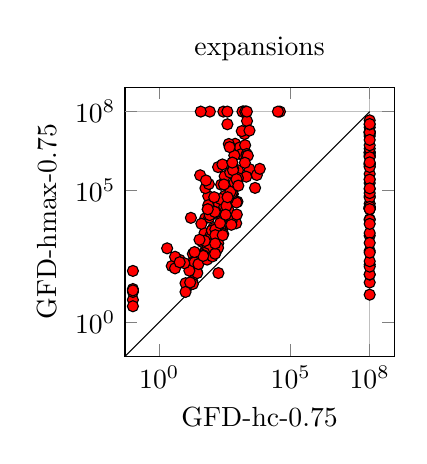
\begin{tikzpicture}
\begin{axis}[extra x tick style={grid=major}, extra x ticks=100000000, extra y tick style={grid=major}, extra y ticks=100000000, height=5cm, legend cell align=left, legend style={at=(1.3, 0.5)}, title=expansions, width=5cm, xlabel=GFD-hc-0.75, xmin=0.05, xmode=log, ylabel=GFD-hmax-0.75, ymin=0.05, ymode=log]
\addplot[color=red, mark=*, mark options={{draw=black}}, only marks] coordinates {
(19, 392) (27, 215) (623, 8950) (6, 232) (100000000, 1040082) (27, 83) (0.100000, 7) (186, 30239) (845, 5713) (1940, 2054791) (100000000, 267540) (53, 2442) (100000000, 507) (100000000, 32) (391, 33028328) (100000000, 192711) (73, 61548) (604, 74110) (100000000, 1919) (100000000, 21772) (1971, 100000000) (188, 3838) (69, 400) (56, 341) (164, 3428) (24, 89) (0.100000, 4) (26, 368) (1652, 100000000) (170, 1626) (100000000, 11740401) (770, 5968890) (100000000, 994853) (947, 567880) (100000000, 2688956) (622, 74110) (51, 424) (391, 27181) (371, 27525) (564, 6921) (1741, 14114568) (1165, 4348281) (73, 27640) (100000000, 426508) (26, 207) (901, 201439) (100000000, 16382238) (246, 3131) (442, 5894179) (18, 36) (100000000, 2905507) (100000000, 8134) (19, 184) (100000000, 14187316) (100000000, 64) (100000000, 20595) (941, 37611) (100000000, 17495781) (552, 4995) (100000000, 24004) (372, 27235) (0.100000, 14) (207, 3838) (607, 74110) (13, 26) (12, 26) (861, 35149) (3, 135) (173, 778708) (100000000, 19923) (10, 30) (100000000, 16266129) (57, 123268) (100000000, 11) (979, 588688) (1651, 2066634) (56, 8783) (439, 141443) (10, 14) (106, 14089) (730, 203857) (100000000, 153) (2708, 655342) (227, 9176) (19, 28) (100000000, 25106283) (419, 19191) (307, 347898) (36, 380600) (0.100000, 18) (64, 561) (606, 74110) (296, 23696) (100000000, 260647) (142, 464) (175, 987) (1548, 100000000) (1362, 2468825) (100000000, 113756) (28, 73) (4, 110) (226, 166785) (2036, 335904) (306, 61958) (100000000, 2419) (70, 19163) (164, 3838) (144, 14897) (715, 2173671) (103, 1006) (100000000, 840413) (417, 49197) (100000000, 16272316) (15, 32) (22, 185) (499, 483086) (100000000, 65) (100000000, 61582) (275, 100000000) (1844, 5287951) (80, 9432) (31, 160) (48, 359) (84, 100000000) (271, 2230) (100000000, 20830) (100000000, 21565) (100000000, 32546922) (70, 1376) (100000000, 7720) (5143, 389358) (1458, 100000000) (100000000, 128) (100000000, 205) (100000000, 1056281) (137, 441) (52, 1008) (1875, 100000000) (100000000, 5412) (937, 273423) (173, 665) (95, 2286) (112, 3700) (100000000, 2767683) (100000000, 31778) (100, 3031) (100000000, 784718) (100000000, 2217403) (214, 47435) (38725, 100000000) (43, 1113) (2, 635) (2121, 2441914) (68, 649) (136, 3311) (0.100000, 88) (100000000, 1999592) (100000000, 54324) (52, 422) (38, 100000000) (83, 11658) (981, 299347) (359, 25847) (2176, 43967863) (77, 176854) (580, 82375) (100000000, 3916081) (2060, 2086171) (32536, 100000000) (511, 89604) (205, 5733) (335, 12092) (66, 237) (0.100000, 16) (2333, 2104717) (178, 73) (288, 169918) (40, 5446) (396, 55735) (54, 1215) (651, 691186) (253, 979696) (34, 1350) (100000000, 46590097) (100000000, 20848) (1373, 18078718) (2695, 19007847) (106, 313) (4, 304) (46, 353) (100000000, 80015) (639, 590477) (602, 1155505) (47, 327) (100000000, 1024) (136, 2013) (100000000, 1848551) (100000000, 1177399) (2144, 100000000) (6652, 668998) (100000000, 5274492) (129, 15414) (100000000, 120939) (867, 269792) (390, 100000000) (4401, 126004) (259, 2000) (22, 457) (14, 90) (100000000, 8393027) (1805, 1136659) (133, 397) (70, 19440) (9, 173) (60, 241899) (6, 188) (1018, 153341) (134, 970) (16, 9148) (100000000, 33658581) (100000000, 23800) (100000000, 436) (123, 55748) (891, 12261) (474, 4487213) (100000000, 19699)
};
\addplot[color=black] coordinates {(0.050000, 0.050000) (100000000, 100000000)};
\end{axis}
\end{tikzpicture}
	\end{minipage}
	\hfill
	\begin{minipage}{0.2\textwidth}
		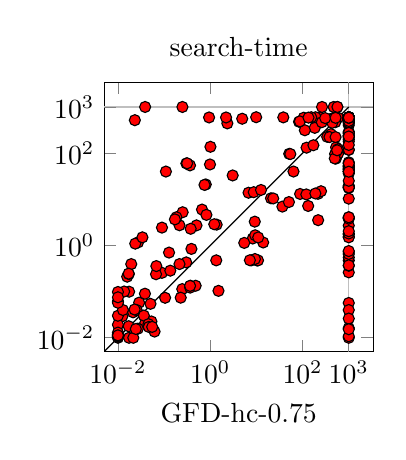
\begin{tikzpicture}
\begin{axis}[extra x tick style={grid=major}, extra x ticks=1000, extra y tick style={grid=major}, extra y ticks=1000, height=5cm, legend cell align=left, legend style={at=(1.3, 0.5)}, title=search-time, width=5cm, xlabel=GFD-hc-0.75, xmin=0.005, xmode=log, ymin=0.005, ymode=log]
\addplot[color=red, mark=*, mark options={{draw=black}}, only marks] coordinates {
(239.686700, 592.492780) (1000, 44.192000) (88.333200, 13.044100) (0.042448, 0.020869) (0.053052, 0.022535) (0.247250, 0.113449) (191.011000, 598.148292) (0.089909, 0.255180) (3.055270, 32.863700) (9.201220, 3.277070) (14.000900, 1.159910) (1000, 596.248911) (1000, 590.760163) (0.105145, 0.073521) (1000, 17.612000) (1000, 586.277640) (1000, 19.074300) (0.390512, 0.842131) (183.374000, 352.888000) (1000, 403.869000) (1000, 0.056717) (10.319500, 0.472343) (1000, 47.640200) (0.109332, 39.898000) (6.745300, 13.862900) (1000, 596.977860) (469.464473, 582.290930) (0.012440, 0.029216) (562.804000, 1000) (0.039041, 0.020883) (1000, 4.071310) (1000, 595.855790) (1000, 533.933219) (1000, 572.406189) (0.301445, 0.429770) (0.010000, 0.019151) (0.010000, 0.010582) (215.791000, 13.141300) (7.773100, 0.475236) (0.021259, 0.035612) (0.662875, 5.988040) (20.672400, 10.509500) (132.023000, 7.168870) (1000, 597.203920) (1000, 1.546220) (0.017457, 0.099556) (1000, 0.473806) (1000, 59.797056) (38.225100, 594.816410) (0.028767, 0.057687) (0.048102, 0.017278) (1000, 595.615664) (1000, 451.476300) (9.873130, 599.618175) (1000, 52.246100) (1000, 0.010000) (0.027270, 1.163310) (1000, 593.627706) (555.458225, 569.479070) (1.347950, 0.475579) (1000, 539.566118) (1000, 595.982655) (1000, 3.877110) (1000, 0.016224) (0.010000, 0.010000) (111.809000, 313.062000) (0.303256, 59.807100) (1000, 595.748590) (0.010000, 0.011690) (1000, 2.685430) (525.440000, 76.005000) (36.526100, 6.943570) (1000, 241.263000) (0.010000, 0.011515) (0.942404, 592.654457) (0.010000, 0.010461) (121.793000, 131.250000) (4.921010, 555.848758) (531.825010, 133.311000) (0.025404, 0.039845) (260.977000, 468.050000) (0.010000, 0.030031) (0.010000, 0.012943) (0.136245, 0.284415) (0.025484, 0.015562) (0.036406, 0.030260) (10.808500, 0.474726) (1000, 0.039864) (1000, 10.323400) (593.356409, 99.361200) (0.252079, 5.239970) (0.249264, 1000) (583.455213, 588.556065) (1000, 580.415522) (0.363576, 54.262400) (410.775138, 257.844000) (0.215185, 2.739420) (2.343780, 441.260000) (1000, 117.477948) (1000, 53.600000) (341.661609, 225.741000) (1000, 595.901620) (0.215148, 0.395105) (250.774000, 14.944000) (0.184662, 4.085290) (83.723600, 478.536000) (1000, 269.901000) (1.505820, 0.103847) (1000, 118.750994) (1000, 18.090500) (0.015850, 0.210763) (512.570000, 468.436010) (587.172135, 122.015000) (1000, 0.261486) (1000, 232.085000) (1000, 0.026059) (1000, 547.139000) (505.890583, 96.037800) (1000, 530.038231) (1000, 39.984000) (1000, 597.191813) (0.798640, 20.957000) (0.017202, 0.241166) (1000, 572.240214) (1000, 50.834600) (63.499600, 39.915300) (1000, 63.260000) (0.023229, 517.355000) (1000, 215.022000) (1000, 1.726980) (0.045755, 0.019723) (0.985828, 56.849600) (1000, 19.605200) (0.502812, 2.721460) (1000, 290.185000) (1000, 541.239470) (1000, 39.948826) (1000, 590.685154) (1000, 1.499690) (1000, 198.042000) (0.023689, 1.095410) (0.010000, 0.010958) (0.038404, 0.090071) (0.228855, 0.073868) (0.373359, 0.133742) (8.727770, 14.257500) (1000, 595.702417) (1000, 543.251770) (0.017363, 0.010000) (1000, 1.818580) (389.122000, 531.027228) (1000, 573.907500) (0.127803, 0.700635) (1000, 553.760517) (1000, 0.010789) (1000, 595.634859) (1000, 3.809670) (0.013625, 0.100590) (439.913876, 454.311000) (120.461000, 12.755900) (9.270080, 0.507900) (0.017076, 0.017768) (1000, 2.039380) (1000, 40.736100) (0.012815, 0.039955) (263.606430, 1000) (0.019416, 0.394944) (1000, 587.589760) (2.198740, 592.393346) (1000, 493.930067) (498.133000, 76.685200) (0.749645, 20.498000) (1000, 584.191260) (0.066841, 0.238087) (189.148000, 13.363700) (12.561000, 15.914900) (0.366348, 0.122053) (1000, 0.550198) (0.062114, 0.013619) (217.206000, 3.529600) (0.033898, 1.498740) (1000, 538.522900) (1000, 584.549331) (171.306000, 148.266000) (0.017055, 0.245152) (1.008210, 137.173000) (0.046551, 0.017173) (7.210440, 0.478286) (8.333380, 1.413950) (1000, 593.912761) (51.318000, 96.532600) (1000, 0.363686) (1.372970, 2.825770) (1000, 45.229200) (0.010000, 0.011279) (153.937000, 598.090278) (54.252600, 95.587500) (5.445150, 1.135540) (1000, 0.015314) (0.171495, 3.671020) (382.171933, 222.993000) (0.021491, 0.010000) (518.004115, 222.577000) (0.022925, 0.041009) (0.027003, 0.015736) (1000, 60.049652) (0.824865, 4.596860) (1000, 0.725662) (0.067908, 0.357078) (1000, 588.851676) (1000, 561.147000) (0.010000, 0.061763) (1000, 483.694200) (1000, 18.049100) (1000, 588.970666) (558.611904, 115.261000) (1000, 36.082500) (471.852767, 1000) (0.050630, 0.054349) (0.482227, 0.133992) (568.061009, 1000) (1000, 25.137900) (1000, 179.867000) (1000, 0.654073) (0.055185, 0.017220) (1000, 0.756189) (1000, 242.950000) (105.635000, 584.497890) (1.220570, 2.878650) (308.857305, 573.897885) (1000, 561.149000) (0.375902, 2.297100) (0.038800, 1000) (0.024382, 0.015493) (1000, 0.371148) (1000, 463.250768) (1000, 4.073550) (1000, 497.026000) (0.010000, 0.098145) (87.188000, 487.605132) (1000, 150.633000) (1000, 39.584834) (9.381180, 1.661590) (23.098400, 10.433000) (1000, 274.179000) (518.101745, 581.973120) (0.010000, 0.057369) (1000, 588.901937) (1000, 229.455000) (0.315012, 60.180200) (0.010000, 0.075327) (50.543000, 8.712060) (0.365297, 0.133167) (10.917000, 1.491440) (0.089867, 2.436060) (1000, 579.203900) (134.172000, 587.822950) (1000, 585.510535)
};
\addplot[color=black] coordinates {(0.0050000, 0.0050000) (1000, 1000)};
\end{axis}
\end{tikzpicture}
	\end{minipage}
	\caption{Comparison of expansions and search time per task of $h^{max}$ and $h^C$ for bounded IPC domains}
\end{figure}

\setlength{\tabcolsep}{1pt}
\begin{figure}[ht]
	\centering
	\scriptsize
	\begin{tabular}{l|rr|rr|rr|rr}
			& \multicolumn{2}{c}{0.25} & \multicolumn{2}{|c}{0.5} & \multicolumn{2}{|c}{0.75}& \multicolumn{2}{|c}{1.0}\\
		& C & max & C & max & C & max & C & hmax\\\hline
		NoMystery 6L 4P & 10 & 10 & 10 & 10 & 10 & 10 & 10 & 10\\
		NoMystery 6L 5P & 10 & 10 & 10 & 10 & 10 & 10 & 10 & 10\\
		NoMystery 6L 6P & 10 & 10 & 10 & 10 & 10 & 10 & 1100 & 10\\
		NoMystery 8L 4P & 10 & 10 & 10 & 10 & 10 & 10 & 9 & 10\\
		NoMystery 8L 5P & 10 & 10 & 10 & 10 & 8 & 10 & 5 & 10\\
		NoMystery 8L 6P & 10 & 10 & 10 & 10 & 8 & 10 & 3 & 7\\
		TPP 6M 4G & 10 & 10 & 10 & 10 & 10 & 10 & 10 & 10\\
		TPP 6M 5G & 10 & 10 & 10 & 10 & 10 & 10 & 10 & 10\\
		TPP 6M 6G & 10 & 10 & 10 & 10 & 10 & 10 & 10 & 10\\
		TPP 6M 7G & 10 & 10 & 10 & 10 & 1 & 8 & 2 & 10\\
		TPP 8M 4G & 10 & 10 & 10 & 10 & 10 & 10 & 10 & 10\\
		TPP 8M 5G & 10 & 10 & 10 & 10 & 10 & 10 & 10 & 10\\
		TPP 8M 6G & 10 & 10 & 10 & 10 & 6 & 10 & 9 & 10\\
		TPP 10M 4G & 10 & 10 & 10 & 10 & 10 & 10 & 10 & 10\\
		TPP 10M 5G & 10 & 10 & 10 & 10 & 10 & 10 & 10 & 10\\
		TPP 10M 6G & 10 & 10 & 10 & 10 & 9 & 10 & 8 & 10\\\hline
		sum \numtasks{160} & 160 & 160 & 160 & 160 & 138 & 158 & 136 & 157\\
	\end{tabular}
	\caption{Coverage: computation of \emph{Goal-Fact Dependencies 1} of the RPC 
		domains with bound $ = x \cdot $ optimal cost with $ x \in \{0.25, 0.5, 0.75\}$
	of online learned dead-end detectors with bounded DFS (C) and $h^{max}$ with $A^*$. 
	time-out 10 min}
\end{figure}

\begin{figure}[ht]
	\begin{minipage}{0.2\textwidth}
		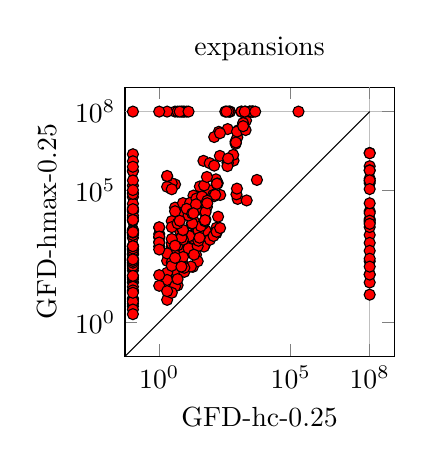
\begin{tikzpicture}
\begin{axis}[extra x tick style={grid=major}, extra x ticks=100000000, extra y tick style={grid=major}, extra y ticks=100000000, height=5cm, legend cell align=left, legend style={at=(1.3, 0.5)}, title=expansions, width=5cm, xlabel=GFD-hc-0.25, xmin=0.05, xmode=log, ylabel=GFD-hmax-0.25, ymin=0.05, ymode=log]
\addplot[color=red, mark=*, mark options={{draw=black}}, only marks] coordinates {
(0.100000, 2971) (14, 1892) (100000000, 840413) (0.100000, 2446) (58, 3037) (100000000, 2688956) (3, 706) (48, 1342391) (0.100000, 811) (4, 170892) (100000000, 65) (208, 67738) (0.100000, 21631) (0.100000, 730) (668, 1368076) (19, 1534) (100000000, 2048) (1019, 19611126) (0.100000, 32) (100000000, 2617617) (18, 1954) (55, 892) (3558, 100000000) (2, 213) (494, 100000000) (9, 496) (25, 364) (4, 22448) (0.100000, 2397766) (13, 636) (649, 2261740) (9, 1572) (0.100000, 4) (8, 33393) (819, 6917972) (958, 47992) (0.100000, 1591) (480, 100000000) (1, 2242) (0.100000, 245) (0.100000, 58) (0.100000, 256) (20, 64248) (0.100000, 553753) (0.100000, 16051) (100000000, 4096) (0.100000, 187) (1, 3844) (0.100000, 166) (1332, 100000000) (0.100000, 2506) (149, 2378) (100000000, 192711) (2768, 100000000) (100000000, 8192) (1, 1108) (3, 344) (1997, 45935775) (14, 1861) (863, 71716) (0.100000, 2323) (196523, 100000000) (0.100000, 56875) (4, 1109) (1908, 100000000) (5, 826) (1, 745) (164, 198133) (0.100000, 19141) (0.100000, 154345) (100000000, 283576) (0.100000, 17761) (0.100000, 3286) (9, 109) (0.100000, 217) (0.100000, 14) (2684, 100000000) (0.100000, 219) (50, 5809) (43, 36387) (0.100000, 745) (0.100000, 9131) (0.100000, 16896) (6, 12007) (9, 100000000) (17, 5356) (31, 3001) (100000000, 587761) (4, 1108) (15, 34032) (0.100000, 226) (0.100000, 379) (8, 152) (0.100000, 11285) (78, 104720) (6, 3101) (45, 5283) (0.100000, 548746) (50, 741) (0.100000, 772) (1563, 28711853) (21, 6526) (40, 18270) (25, 19579) (100000000, 232531) (100000000, 16384) (100000000, 580396) (426, 100000000) (0.100000, 33) (5, 73) (1, 4035) (65, 23798) (11, 100000000) (29, 764) (4, 347) (395, 1143601) (0.100000, 5) (0.100000, 586) (0.100000, 7615) (85, 1355) (801, 7341225) (0.100000, 8) (19, 126) (931, 10420707) (2, 7) (0.100000, 246) (35, 142466) (2109, 42030) (26, 49620) (83, 1096038) (2, 50) (3, 188791) (112, 67588) (0.100000, 370) (2, 138858) (3, 112017) (38, 4427) (29, 205) (9, 81) (100000000, 13979) (151, 3851) (7, 100000000) (0.100000, 7) (8, 1360) (100000000, 1024) (3, 962) (4, 100000000) (3, 6886) (116, 1880) (51, 156560) (409, 1131640) (8, 100000000) (400, 21653693) (902, 118208) (5, 100000000) (3, 21) (0.100000, 43) (4, 1241) (100000000, 32) (123, 884552) (3510, 100000000) (0.100000, 151) (0.100000, 2566) (2841, 100000000) (3709, 100000000) (0.100000, 2056) (2, 19) (0.100000, 559) (0.100000, 15) (803, 5975018) (100000000, 6272) (1, 1627) (2, 75) (0.100000, 50) (907, 17460317) (8, 297) (18, 5647) (122, 60875) (5183, 252962) (7, 1627) (31, 1236) (8, 3101) (184, 17075893) (0.100000, 7036) (42, 59583) (0.100000, 22) (0.100000, 91) (155, 185045) (6, 100000000) (824, 6722843) (0.100000, 3076) (3, 1438) (0.100000, 113) (0.100000, 31561) (13, 11292) (8, 3160) (100000000, 7138) (0.100000, 19591) (4, 803) (1920, 19918398) (0.100000, 136) (2, 346276) (0.100000, 407) (0.100000, 100000000) (151, 2707) (3, 4066) (2, 357856) (100000000, 244221) (2, 40) (143, 266816) (57, 8012) (100000000, 205) (16, 129) (0.100000, 6) (11, 20161) (1, 1780) (100000000, 64) (0.100000, 1294345) (135, 69035) (5, 5617) (54, 6870) (4, 16278) (100000000, 113756) (0.100000, 181) (3249, 100000000) (58, 15290) (0.100000, 2521) (65, 328078) (100000000, 512) (166, 185292) (100000000, 32768) (0.100000, 16) (0.100000, 241546) (1334, 100000000) (1, 1053) (0.100000, 3) (0.100000, 507) (3, 187) (391, 846921) (6, 7076) (100000000, 5412) (325, 100000000) (2, 100000000) (9, 116) (0.100000, 802036) (0.100000, 57) (3, 138) (55, 7441) (1776, 100000000) (0.100000, 2791) (67, 40955) (0.100000, 211) (5, 25) (4, 23) (4451, 100000000) (156, 182080) (0.100000, 7625) (2, 406) (34, 1614) (0.100000, 2626) (13, 100000000) (18, 13376) (1, 24) (1542, 36749162) (123, 10801620) (100000000, 256) (3, 13) (204, 15117895) (0.100000, 632) (173, 10156) (0.100000, 241) (1, 61) (25, 29955) (202, 2073240) (7, 128) (100000000, 11) (4, 276) (0.100000, 80806) (100000000, 128) (416, 1656947) (5, 43) (0.100000, 13) (0.100000, 2) (67, 32916) (0.100000, 74443) (0.100000, 766) (206, 3759) (1, 100000000) (21, 365) (2, 15) (1, 573) (20, 13650) (362, 100000000) (0.100000, 104311) (1545, 27889713)
};
\addplot[color=black] coordinates {(0.050000, 0.050000) (100000000, 100000000)};
\end{axis}
\end{tikzpicture}
	\end{minipage}
	\hfill
	\begin{minipage}{0.2\textwidth}
		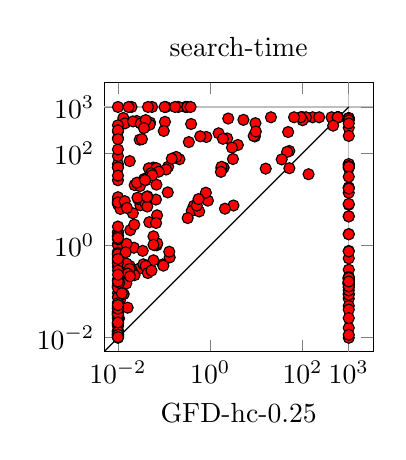
\begin{tikzpicture}
\begin{axis}[extra x tick style={grid=major}, extra x ticks=1000, extra y tick style={grid=major}, extra y ticks=1000, height=5cm, legend cell align=left, legend style={at=(1.3, 0.5)}, title=search-time, width=5cm, xlabel=GFD-hc-0.25, xmin=0.005, xmode=log, ymin=0.005, ymode=log]
\addplot[color=red, mark=*, mark options={{draw=black}}, only marks] coordinates {
(0.028531, 0.314060) (0.010000, 0.141879) (0.069130, 1.009340) (0.214463, 73.840300) (1000, 47.512000) (1000, 18.145400) (164.948000, 598.097963) (0.010000, 0.020384) (0.888732, 9.357150) (0.010000, 0.010339) (0.010547, 0.026249) (0.010000, 9.696930) (1.949160, 48.497200) (0.010114, 0.348226) (0.035558, 0.390635) (0.030658, 7.416310) (0.020102, 0.282966) (0.093627, 0.389600) (1000, 0.146346) (0.010000, 0.037258) (0.047734, 3.195270) (0.054777, 1000) (0.010000, 0.018990) (0.010000, 0.027059) (0.010000, 291.270000) (1000, 0.070376) (1000, 569.424419) (1000, 0.147251) (0.010000, 0.011000) (0.010000, 0.014282) (0.010000, 0.032966) (9.261430, 229.940000) (1000, 13.833200) (568.991588, 598.365640) (1000, 56.506600) (0.010000, 0.093661) (0.010000, 0.625783) (0.010000, 212.797000) (1000, 57.913900) (585.815451, 599.292347) (0.018514, 2.145660) (0.030658, 23.419100) (0.058698, 0.476285) (0.010000, 0.124818) (0.039912, 0.360602) (1000, 0.298156) (0.010000, 0.032660) (0.010000, 0.441437) (0.441380, 7.235470) (1000, 52.462000) (1000, 0.526094) (0.010000, 0.739707) (0.109002, 1000) (0.010000, 0.128580) (0.010000, 0.533941) (0.044337, 0.253154) (8.732200, 236.280000) (0.821598, 223.901000) (0.010000, 0.349141) (0.010000, 0.415298) (0.010000, 0.012020) (51.444700, 111.268000) (1000, 0.200383) (1000, 0.155744) (1000, 0.122064) (0.010000, 0.125091) (0.010000, 0.654800) (0.058423, 48.598600) (0.017100, 0.215000) (0.018001, 67.173300) (0.049603, 459.697721) (0.010000, 1000) (0.062464, 1.013790) (0.070845, 1.111720) (0.022982, 20.293900) (0.010000, 0.010941) (0.010000, 0.010000) (0.010000, 1.087460) (0.010000, 57.810300) (1000, 0.149782) (1000, 0.089930) (0.010000, 0.047572) (1000, 0.188603) (0.010000, 1.914130) (1000, 0.161828) (0.010000, 1.004810) (0.027428, 10.144400) (1000, 0.085536) (0.010000, 0.691930) (0.289593, 1000) (0.070357, 4.489520) (1000, 550.260712) (2.323220, 208.309000) (1000, 578.774518) (228.567000, 598.501116) (1000, 560.307000) (1.744380, 46.789000) (0.017942, 0.359657) (0.017776, 0.221800) (0.010000, 8.325430) (0.037782, 27.362300) (0.802361, 13.916800) (0.384356, 427.486000) (0.104265, 475.926000) (0.010000, 0.011866) (0.010930, 0.047907) (0.010000, 0.662245) (0.013085, 576.713000) (0.010000, 0.020199) (0.010000, 0.560587) (0.010000, 48.464000) (0.015242, 0.407146) (1000, 17.712200) (0.122342, 50.788600) (94.658300, 598.357417) (0.010000, 0.031758) (0.046649, 46.875400) (3.955460, 150.179000) (0.010000, 8.375120) (1.745930, 50.451300) (0.010381, 0.663351) (0.096368, 0.365264) (0.010000, 0.021505) (0.010000, 0.031001) (0.010000, 8.778260) (0.010000, 0.644579) (1000, 0.048968) (0.058784, 1.575660) (0.011130, 0.065548) (0.021027, 4.983350) (9.504350, 445.596445) (423.753000, 597.979372) (1000, 0.208494) (0.010000, 7.778180) (1.700400, 39.241200) (0.010000, 0.020862) (0.068110, 20.766900) (0.010000, 0.498735) (0.010000, 0.012132) (0.019643, 1000) (0.025550, 495.998221) (46.195600, 106.286177) (1000, 355.522000) (0.203845, 1000) (0.010000, 0.017955) (580.252808, 597.421969) (0.010000, 0.033312) (0.010000, 0.035483) (1000, 0.157770) (0.011288, 6.192890) (0.098322, 302.164000) (0.039069, 8.381740) (0.397300, 5.635290) (0.053284, 0.285385) (0.010000, 0.057473) (100.975000, 598.216867) (0.010000, 0.025870) (1000, 0.195165) (0.010000, 0.010978) (0.010000, 1.975790) (0.010000, 0.043581) (0.172095, 1000) (0.010000, 1.590360) (15.893100, 46.122117) (1000, 4.261360) (1000, 1.757520) (580.598600, 594.655141) (1000, 7.611890) (0.016215, 0.044811) (0.043216, 6.965240) (0.014153, 441.236015) (0.013324, 0.088213) (0.067668, 47.186100) (0.010000, 0.185382) (0.010000, 0.076204) (584.028800, 596.980998) (1000, 0.016357) (0.010000, 11.088200) (0.039464, 25.813500) (0.021167, 486.462518) (1000, 511.635237) (0.048727, 413.388000) (1000, 0.760297) (0.182816, 82.580300) (0.010000, 0.074801) (20.621400, 598.119890) (0.022172, 0.892949) (0.015340, 1.087410) (0.132199, 0.551221) (0.010000, 8.553830) (0.066446, 9.857860) (0.022853, 0.227104) (0.014732, 0.711961) (0.010000, 0.013969) (0.044813, 1000) (5.221790, 525.968498) (0.016285, 0.207687) (0.036913, 27.439100) (35.287900, 73.143364) (0.029990, 19.276300) (0.029580, 195.461000) (0.010000, 0.035689) (0.010000, 0.133593) (0.010000, 25.876100) (0.110527, 44.192400) (0.102309, 1000) (0.010000, 0.056058) (118.557000, 597.986894) (0.010000, 0.013781) (0.025675, 22.855600) (100.015000, 516.268905) (0.010000, 400.294000) (0.010000, 0.044326) (0.010000, 0.027529) (0.016945, 1000) (1000, 17.061700) (593.707266, 595.013936) (0.010000, 0.414810) (2.951390, 131.703000) (1000, 7.956260) (3.176630, 7.332720) (0.076434, 39.598700) (1000, 0.010000) (1.516048, 269.118000) (0.010000, 1.627680) (3.097730, 74.544600) (0.031105, 437.880117) (0.010000, 0.043703) (0.010000, 0.049372) (0.013997, 9.101260) (1000, 4.270620) (0.040016, 519.573000) (0.052631, 36.732000) (0.010000, 0.010387) (0.017830, 0.310687) (0.010000, 1.576880) (0.010000, 0.120594) (0.010000, 1.353550) (0.010000, 0.030457) (0.043659, 11.569400) (1000, 50.341200) (0.010000, 86.735000) (1000, 0.178393) (0.010000, 119.999000) (0.010000, 0.013099) (0.010000, 0.018442) (1000, 0.740091) (0.317699, 1000) (0.016285, 0.246044) (0.010000, 0.011925) (91.138600, 598.361146) (0.146924, 75.848100) (0.575185, 5.450780) (0.010000, 49.201700) (1000, 0.106344) (1000, 0.153929) (0.010000, 0.036721) (0.012169, 0.091736) (0.509863, 7.281820) (48.657400, 286.284000) (65.293700, 598.130903) (0.010000, 32.505000) (0.058824, 1.032870) (2.447110, 562.072608) (0.010000, 2.568680) (0.342952, 173.454000) (0.010000, 0.032530) (0.010000, 0.013371) (0.015131, 0.149984) (2.080980, 6.257675) (0.120053, 14.097800) (0.010000, 1.456300) (0.605574, 231.769000) (0.026458, 10.813300) (0.036528, 348.712000) (0.010651, 0.155582) (0.010000, 0.173754) (0.034320, 0.764386) (1000, 439.919507) (0.010000, 0.287413) (9.697540, 293.971000) (1.879740, 204.617000) (0.015641, 6.487840) (51.669200, 47.105461) (1000, 0.143147) (0.010000, 0.013457) (1000, 0.040705) (581.975225, 598.321136) (1000, 0.195246) (1000, 0.158616) (1000, 0.197603) (0.042501, 11.368500) (0.556439, 10.099300) (0.010000, 0.011628) (0.010000, 0.510173) (0.018328, 0.213925) (573.652052, 596.079760) (1000, 0.026707) (575.292850, 597.331070) (0.022572, 2.822820) (0.324084, 3.919240) (0.010000, 0.042692) (1000, 0.129543) (0.010000, 0.011598) (0.374536, 1000) (0.010000, 312.369000) (1000, 0.011587) (0.010000, 0.050968) (0.129126, 0.730525) (1000, 235.834000) (0.067089, 3.069910) (0.055317, 33.004900) (0.010000, 0.166198) (0.033064, 200.660000) (134.652364, 34.887698) (1000, 30.773200) (0.010000, 0.010325) (458.991556, 394.041305) (0.010000, 201.330000) (0.010000, 0.021533) (1000, 0.165509) (1000, 1.747380) (0.010032, 0.233055) (0.038649, 26.114200)
};
\addplot[color=black] coordinates {(0.0050000, 0.0050000) (1000, 1000)};
\end{axis}
\end{tikzpicture}
	\end{minipage}

	\begin{minipage}{0.2\textwidth}
		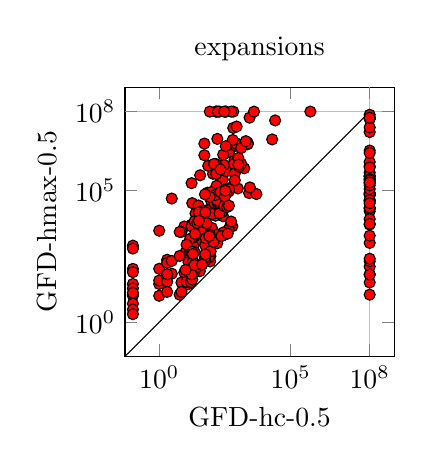
\begin{tikzpicture}
\begin{axis}[extra x tick style={grid=major}, extra x ticks=100000000, extra y tick style={grid=major}, extra y ticks=100000000, height=5cm, legend cell align=left, legend style={at=(1.3, 0.5)}, title=expansions, width=5cm, xlabel=GFD-hc-0.5, xmin=0.05, xmode=log, ylabel=GFD-hmax-0.5, ymin=0.05, ymode=log]
\addplot[color=red, mark=*, mark options={{draw=black}}, only marks] coordinates {
(652, 23964757) (194, 100000000) (28, 1247) (147, 100000000) (100000000, 11) (100000000, 840413) (326, 100000000) (100000000, 16702396) (179, 14491) (68, 82576) (100000000, 65) (602, 4359) (24, 13367) (59, 264) (3, 69) (259, 263094) (100000000, 270832) (417, 25540) (54, 1966) (63, 17624) (1, 28) (100000000, 128) (100000000, 205) (88, 319) (20, 198) (10, 447) (729, 1451467) (93, 41213) (2, 233) (100000000, 1024) (386, 92308) (1025, 997124) (521, 5111) (100000000, 20981) (1, 10) (100000000, 52302447) (144, 100000000) (347, 2631585) (649, 4842364) (70, 2924) (1, 106) (100000000, 192711) (137, 11063) (155, 36643) (150, 36643) (86, 202) (803, 6434752) (12, 39) (151, 150205) (18, 89) (52, 6085027) (145, 36643) (1, 38) (2, 49) (36, 380600) (460, 115325) (266, 10562) (78, 1815) (17, 5009) (0.100000, 10) (52, 2196973) (100000000, 74322) (349, 100000000) (443, 2938657) (100000000, 38907) (12, 27) (100000000, 32) (269, 2318245) (223, 817242) (77, 284) (187, 14177) (432, 3279) (20, 776) (0.100000, 105) (126, 34084) (100, 3806) (100000000, 81330) (2614, 80074) (100000000, 3309201) (727, 450815) (78, 1060) (111, 433598) (0.100000, 11) (100000000, 65313) (9, 77) (100000000, 16384) (493, 125022) (159, 36643) (0.100000, 28) (974, 119944) (443, 91606) (24, 98) (17, 4715) (18, 33187) (35, 86) (1233, 932069) (6, 11) (100000000, 482812) (100000000, 1222697) (9, 4284) (1, 2984) (0.100000, 5) (20, 147) (543, 6627) (19675, 8761602) (31, 27029) (21, 76) (105, 12812) (449, 111835) (23, 147) (160, 987) (92, 86481) (29, 6515) (7, 32) (23, 5902) (2282, 6685177) (56, 836) (100000000, 59040002) (242, 15037) (84, 100000000) (22, 1800) (354, 77219) (793, 5077544) (652, 100000000) (7, 2696) (30, 137) (158, 42285) (6, 2675) (100000000, 42073) (2, 179) (33, 6745) (195, 13504) (18, 1573) (100000000, 348502) (75, 1846) (40, 2772) (164, 2125) (162, 9193600) (100000000, 337294) (147, 427926) (2, 34) (172, 100000000) (2726, 58800144) (678, 1023342) (133, 67358) (13, 230) (100000000, 1919) (100000000, 72844) (272, 1989) (100000000, 205227) (296, 25836) (11, 34) (4008, 100000000) (277, 2558) (352, 540153) (46, 16621) (82, 1846) (56, 225) (7, 14) (289, 933590) (55, 282) (17, 4295) (63, 5710) (100000000, 113756) (16, 33) (13, 190) (0.100000, 747) (90, 490) (2, 14) (27, 124) (100000000, 75797336) (22, 6819) (100000000, 58708639) (213, 87835) (0.100000, 19) (17, 190693) (28, 5833) (100000000, 5058) (0.100000, 807) (2228, 5730375) (83, 57753) (100000000, 20595) (100000000, 64) (100000000, 364225) (19, 202) (56, 378) (310, 59125) (32, 14940) (84, 2100) (18, 41) (1707, 700030) (115, 1104) (15, 520) (737, 444814) (17, 65) (22, 464) (22, 147) (551, 100000000) (100000000, 43567) (146, 1007174) (2159, 5841704) (3, 211) (15, 1458) (1069, 811635) (295, 100000000) (10, 96) (1302, 1048225) (100000000, 270540) (0.100000, 3) (381, 23581) (100000000, 244805) (57, 14941) (43, 153) (2352, 6018469) (3, 49622) (0.100000, 622) (835, 6074570) (25480, 46273952) (59, 1526) (1017, 1730892) (100000000, 22374) (100000000, 755522) (2, 66) (73, 865105) (446, 26597) (100000000, 256) (231, 1852) (625, 8328784) (340, 4845380) (11, 876) (100000000, 8192) (100000000, 2688956) (100000000, 157425) (100000000, 25106283) (100000000, 201980) (100000000, 57729847) (323, 98315) (100000000, 33063) (80, 1846) (401, 2296) (100000000, 5412) (745, 243614) (121, 1023724) (4955, 73726) (18, 474) (876, 27067605) (1304, 4123680) (6, 327) (55, 71498) (0.100000, 79) (32, 7110) (212, 635569) (23, 2237) (0.100000, 13) (19, 386) (0.100000, 2) (1960, 7525022) (556807, 100000000) (1028, 965313) (2800, 131570)
};
\addplot[color=black] coordinates {(0.050000, 0.050000) (100000000, 100000000)};
\end{axis}
\end{tikzpicture}
	\end{minipage}
	\hfill
	\begin{minipage}{0.2\textwidth}
		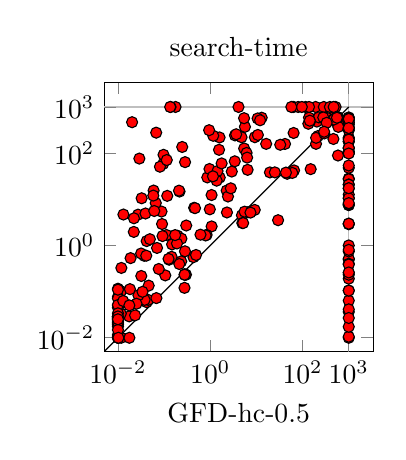
\begin{tikzpicture}
\begin{axis}[extra x tick style={grid=major}, extra x ticks=1000, extra y tick style={grid=major}, extra y ticks=1000, height=5cm, legend cell align=left, legend style={at=(1.3, 0.5)}, title=search-time, width=5cm, xlabel=GFD-hc-0.5, xmin=0.005, xmode=log, ymin=0.005, ymode=log]
\addplot[color=red, mark=*, mark options={{draw=black}}, only marks] coordinates {
(0.041854, 0.058998) (0.017512, 0.029074) (583.951830, 578.087266) (0.037065, 0.597193) (0.011856, 0.325930) (562.098282, 570.258813) (0.234970, 0.452103) (0.095245, 58.273000) (4.848530, 4.508220) (0.010000, 0.019311) (0.861978, 29.773200) (65.362500, 42.249900) (1000, 212.089324) (0.013125, 4.676810) (466.213000, 593.853868) (0.031718, 0.669523) (0.246724, 135.894000) (0.010000, 0.028847) (0.045140, 0.066215) (578.217781, 569.525860) (0.037833, 0.066226) (0.215847, 14.712000) (1.601492, 29.499500) (191.180600, 1000) (6.540580, 5.245030) (0.010000, 0.010042) (1000, 413.468000) (1000, 28.137200) (63.917500, 1000) (116.044900, 1000) (195.385000, 158.980346) (0.010000, 0.027245) (137.798000, 588.061800) (0.449681, 0.586254) (2.923400, 39.887900) (1000, 27.132800) (1000, 178.287123) (0.097101, 91.953100) (0.010000, 0.017650) (1.066810, 12.365600) (1.069230, 2.583420) (0.010000, 0.024115) (0.196374, 1.618480) (0.027724, 0.083583) (0.106003, 0.224642) (589.323401, 424.172000) (0.276432, 0.120557) (137.913000, 1000) (0.018779, 0.531310) (298.563300, 565.755300) (586.411735, 501.082590) (215.539000, 234.637000) (0.176659, 1000) (0.070280, 0.882896) (0.137911, 1000) (1000, 455.694400) (0.011648, 0.102102) (5.522910, 5.392900) (1000, 0.190798) (1000, 0.010000) (2.265700, 15.438200) (331.121500, 584.845830) (0.010000, 0.021178) (0.010000, 0.026272) (567.056913, 584.249175) (571.506110, 593.732757) (1000, 0.010558) (574.517335, 564.899979) (287.868000, 1000) (0.301398, 2.703370) (0.284444, 63.782600) (0.010000, 0.010000) (0.961149, 45.271200) (0.010000, 0.051108) (1000, 100.360018) (0.281107, 0.230384) (462.047500, 536.881400) (1000, 100.205057) (1.590130, 218.728000) (521.481018, 566.063397) (203.939000, 482.329000) (0.032044, 0.217965) (1000, 512.057896) (1000, 0.063750) (0.010000, 0.010808) (1000, 0.036456) (0.210360, 15.388900) (1000, 568.279600) (1000, 107.623000) (1000, 593.717716) (0.158121, 1.608910) (1000, 20.903804) (0.297253, 0.232706) (1000, 354.828228) (259.726990, 593.197490) (478.359803, 1000) (2.297260, 5.185390) (0.010000, 0.025250) (579.021152, 593.814848) (59.386504, 1000) (0.027262, 4.648260) (19.599300, 38.239400) (0.447559, 6.548910) (1000, 10.593297) (1000, 0.493199) (1000, 7.462530) (41.617210, 158.059000) (1000, 0.105815) (46.388700, 35.714100) (592.167364, 591.707802) (1000, 2.968010) (553.195883, 578.374876) (1000, 103.731000) (0.237001, 1.405810) (0.010000, 0.028545) (223.793300, 595.052587) (537.874753, 562.740729) (9.247950, 221.428000) (0.018215, 0.113035) (1000, 1.000170) (1000, 0.256493) (1000, 0.017302) (1000, 573.958000) (1000, 0.232753) (0.148965, 1.054250) (196.353000, 214.566000) (584.748496, 88.786300) (0.041061, 0.600610) (1000, 214.752031) (0.832867, 1.691500) (0.010000, 0.076989) (2.418060, 11.496100) (0.087744, 5.424880) (5.633600, 371.417000) (595.752315, 591.951122) (0.010000, 0.071111) (1.374770, 25.320300) (9.179850, 5.884340) (1000, 48.045600) (583.857618, 408.846000) (465.185676, 202.442000) (80.251000, 1000) (1000, 0.516748) (0.112633, 1.681790) (1.548280, 117.954000) (1000, 20.741555) (0.010000, 0.026762) (582.970766, 541.620603) (280.171700, 593.289740) (145.512000, 491.027000) (96.254700, 1000) (4.945770, 3.053140) (1000, 0.401467) (10.741100, 247.753000) (0.010000, 0.011544) (1000, 7.587580) (0.081195, 50.735000) (1000, 464.929000) (0.010000, 0.028895) (556.176868, 587.599603) (0.011523, 0.033378) (1000, 128.040106) (0.065914, 8.298160) (3.429660, 242.416000) (1000, 0.104959) (0.059249, 15.471600) (25.077300, 38.284300) (0.039527, 4.927230) (0.128162, 0.491366) (0.793168, 1.645930) (552.808508, 582.840500) (1000, 177.756549) (12.993800, 585.597000) (1000, 311.801000) (1000, 128.592087) (4.756960, 221.012000) (0.432123, 0.557127) (1000, 0.741736) (1.435160, 40.935400) (1000, 560.617000) (0.020234, 467.538000) (1000, 2.878550) (29.455000, 3.524120) (594.747380, 442.858000) (133.238000, 432.464719) (1000, 2.962560) (0.025246, 0.054664) (0.280537, 0.237662) (0.092348, 1.595900) (5.416010, 126.186000) (0.282976, 0.747016) (518.874000, 1000) (0.068022, 0.072295) (0.010000, 0.045028) (1000, 0.386447) (390.000274, 1000) (1000, 196.416000) (1000, 104.227107) (59.936600, 37.253700) (4.090460, 1000) (1000, 345.154000) (1.762370, 59.899100) (555.527832, 599.244595) (0.061185, 5.575570) (1000, 17.134600) (0.189999, 1.105200) (32.797900, 151.754000) (6.440810, 43.456800) (0.116939, 11.854800) (0.010000, 0.051285) (0.022049, 1.964370) (43.525400, 37.900300) (0.011750, 0.010000) (3.645580, 256.275000) (0.010000, 0.115553) (0.491521, 0.621463) (0.467532, 6.430830) (1000, 130.040593) (0.010000, 0.020605) (5.396610, 571.010420) (0.041911, 1.242690) (0.010000, 0.022080) (0.067357, 277.610000) (0.017679, 0.010000) (0.046295, 0.134812) (470.489084, 1000) (570.960153, 547.962000) (0.114115, 70.780500) (63.894000, 273.248000) (594.523589, 370.082000) (0.010000, 0.033875) (1000, 353.036076) (0.022196, 3.878580) (1000, 12.660100) (6.118860, 100.904000) (0.032585, 10.520500) (0.173316, 1.674720) (476.660545, 534.311070) (0.058332, 12.029800) (0.010012, 0.010000) (0.012982, 0.062723) (0.010000, 0.029008) (1000, 54.021300) (1.159770, 237.523000) (1000, 0.802083) (1000, 10.501917) (2.787500, 17.274100) (0.213208, 0.396295) (0.029096, 76.185300) (0.976845, 6.063030) (0.010000, 0.014844) (1000, 7.854510) (0.145127, 0.567423) (331.623400, 453.572900) (143.091000, 504.077015) (5.151120, 3.058870) (0.124741, 0.511678) (0.010223, 0.010000) (575.238170, 597.014617) (1000, 98.251900) (1000, 0.041238) (0.010000, 0.110222) (0.023540, 0.030603) (1.143190, 31.443100) (0.943874, 314.032000) (57.114800, 1000) (149.497000, 44.966500) (0.090176, 2.911880) (1000, 549.940000) (294.942900, 267.237000) (292.622000, 290.795000) (1000, 349.690000) (0.076476, 0.309012) (555.730720, 584.573110) (0.135479, 1000) (0.613292, 1.712940) (1000, 0.260186) (1000, 0.026837) (0.034045, 0.099102) (3.394820, 66.499800) (10.604200, 564.033346) (0.277461, 0.232817) (1000, 8.248860) (6.293030, 80.004400) (7.425210, 5.145460) (0.049207, 1.366350) (0.017666, 0.050313) (16.253600, 158.675000) (0.010000, 0.025130) (11.985100, 514.434511) (1000, 17.380700)
};
\addplot[color=black] coordinates {(0.0050000, 0.0050000) (1000, 1000)};
\end{axis}
\end{tikzpicture}
	\end{minipage}

	\begin{minipage}{0.2\textwidth}
		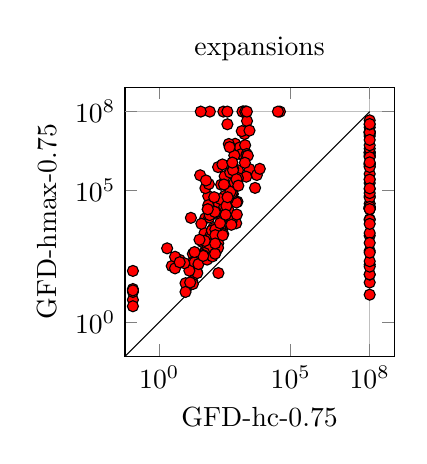
\begin{tikzpicture}
\begin{axis}[extra x tick style={grid=major}, extra x ticks=100000000, extra y tick style={grid=major}, extra y ticks=100000000, height=5cm, legend cell align=left, legend style={at=(1.3, 0.5)}, title=expansions, width=5cm, xlabel=GFD-hc-0.75, xmin=0.05, xmode=log, ylabel=GFD-hmax-0.75, ymin=0.05, ymode=log]
\addplot[color=red, mark=*, mark options={{draw=black}}, only marks] coordinates {
(19, 392) (27, 215) (623, 8950) (6, 232) (100000000, 1040082) (27, 83) (0.100000, 7) (186, 30239) (845, 5713) (1940, 2054791) (100000000, 267540) (53, 2442) (100000000, 507) (100000000, 32) (391, 33028328) (100000000, 192711) (73, 61548) (604, 74110) (100000000, 1919) (100000000, 21772) (1971, 100000000) (188, 3838) (69, 400) (56, 341) (164, 3428) (24, 89) (0.100000, 4) (26, 368) (1652, 100000000) (170, 1626) (100000000, 11740401) (770, 5968890) (100000000, 994853) (947, 567880) (100000000, 2688956) (622, 74110) (51, 424) (391, 27181) (371, 27525) (564, 6921) (1741, 14114568) (1165, 4348281) (73, 27640) (100000000, 426508) (26, 207) (901, 201439) (100000000, 16382238) (246, 3131) (442, 5894179) (18, 36) (100000000, 2905507) (100000000, 8134) (19, 184) (100000000, 14187316) (100000000, 64) (100000000, 20595) (941, 37611) (100000000, 17495781) (552, 4995) (100000000, 24004) (372, 27235) (0.100000, 14) (207, 3838) (607, 74110) (13, 26) (12, 26) (861, 35149) (3, 135) (173, 778708) (100000000, 19923) (10, 30) (100000000, 16266129) (57, 123268) (100000000, 11) (979, 588688) (1651, 2066634) (56, 8783) (439, 141443) (10, 14) (106, 14089) (730, 203857) (100000000, 153) (2708, 655342) (227, 9176) (19, 28) (100000000, 25106283) (419, 19191) (307, 347898) (36, 380600) (0.100000, 18) (64, 561) (606, 74110) (296, 23696) (100000000, 260647) (142, 464) (175, 987) (1548, 100000000) (1362, 2468825) (100000000, 113756) (28, 73) (4, 110) (226, 166785) (2036, 335904) (306, 61958) (100000000, 2419) (70, 19163) (164, 3838) (144, 14897) (715, 2173671) (103, 1006) (100000000, 840413) (417, 49197) (100000000, 16272316) (15, 32) (22, 185) (499, 483086) (100000000, 65) (100000000, 61582) (275, 100000000) (1844, 5287951) (80, 9432) (31, 160) (48, 359) (84, 100000000) (271, 2230) (100000000, 20830) (100000000, 21565) (100000000, 32546922) (70, 1376) (100000000, 7720) (5143, 389358) (1458, 100000000) (100000000, 128) (100000000, 205) (100000000, 1056281) (137, 441) (52, 1008) (1875, 100000000) (100000000, 5412) (937, 273423) (173, 665) (95, 2286) (112, 3700) (100000000, 2767683) (100000000, 31778) (100, 3031) (100000000, 784718) (100000000, 2217403) (214, 47435) (38725, 100000000) (43, 1113) (2, 635) (2121, 2441914) (68, 649) (136, 3311) (0.100000, 88) (100000000, 1999592) (100000000, 54324) (52, 422) (38, 100000000) (83, 11658) (981, 299347) (359, 25847) (2176, 43967863) (77, 176854) (580, 82375) (100000000, 3916081) (2060, 2086171) (32536, 100000000) (511, 89604) (205, 5733) (335, 12092) (66, 237) (0.100000, 16) (2333, 2104717) (178, 73) (288, 169918) (40, 5446) (396, 55735) (54, 1215) (651, 691186) (253, 979696) (34, 1350) (100000000, 46590097) (100000000, 20848) (1373, 18078718) (2695, 19007847) (106, 313) (4, 304) (46, 353) (100000000, 80015) (639, 590477) (602, 1155505) (47, 327) (100000000, 1024) (136, 2013) (100000000, 1848551) (100000000, 1177399) (2144, 100000000) (6652, 668998) (100000000, 5274492) (129, 15414) (100000000, 120939) (867, 269792) (390, 100000000) (4401, 126004) (259, 2000) (22, 457) (14, 90) (100000000, 8393027) (1805, 1136659) (133, 397) (70, 19440) (9, 173) (60, 241899) (6, 188) (1018, 153341) (134, 970) (16, 9148) (100000000, 33658581) (100000000, 23800) (100000000, 436) (123, 55748) (891, 12261) (474, 4487213) (100000000, 19699)
};
\addplot[color=black] coordinates {(0.050000, 0.050000) (100000000, 100000000)};
\end{axis}
\end{tikzpicture}
	\end{minipage}
	\hfill
	\begin{minipage}{0.2\textwidth}
		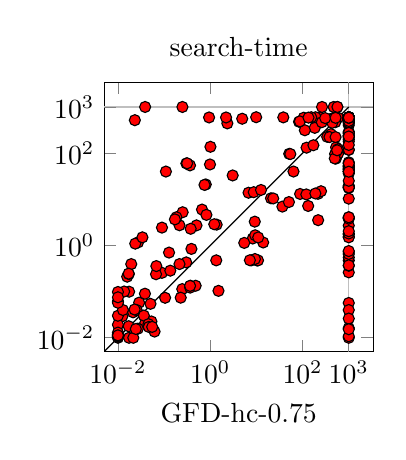
\begin{tikzpicture}
\begin{axis}[extra x tick style={grid=major}, extra x ticks=1000, extra y tick style={grid=major}, extra y ticks=1000, height=5cm, legend cell align=left, legend style={at=(1.3, 0.5)}, title=search-time, width=5cm, xlabel=GFD-hc-0.75, xmin=0.005, xmode=log, ymin=0.005, ymode=log]
\addplot[color=red, mark=*, mark options={{draw=black}}, only marks] coordinates {
(239.686700, 592.492780) (1000, 44.192000) (88.333200, 13.044100) (0.042448, 0.020869) (0.053052, 0.022535) (0.247250, 0.113449) (191.011000, 598.148292) (0.089909, 0.255180) (3.055270, 32.863700) (9.201220, 3.277070) (14.000900, 1.159910) (1000, 596.248911) (1000, 590.760163) (0.105145, 0.073521) (1000, 17.612000) (1000, 586.277640) (1000, 19.074300) (0.390512, 0.842131) (183.374000, 352.888000) (1000, 403.869000) (1000, 0.056717) (10.319500, 0.472343) (1000, 47.640200) (0.109332, 39.898000) (6.745300, 13.862900) (1000, 596.977860) (469.464473, 582.290930) (0.012440, 0.029216) (562.804000, 1000) (0.039041, 0.020883) (1000, 4.071310) (1000, 595.855790) (1000, 533.933219) (1000, 572.406189) (0.301445, 0.429770) (0.010000, 0.019151) (0.010000, 0.010582) (215.791000, 13.141300) (7.773100, 0.475236) (0.021259, 0.035612) (0.662875, 5.988040) (20.672400, 10.509500) (132.023000, 7.168870) (1000, 597.203920) (1000, 1.546220) (0.017457, 0.099556) (1000, 0.473806) (1000, 59.797056) (38.225100, 594.816410) (0.028767, 0.057687) (0.048102, 0.017278) (1000, 595.615664) (1000, 451.476300) (9.873130, 599.618175) (1000, 52.246100) (1000, 0.010000) (0.027270, 1.163310) (1000, 593.627706) (555.458225, 569.479070) (1.347950, 0.475579) (1000, 539.566118) (1000, 595.982655) (1000, 3.877110) (1000, 0.016224) (0.010000, 0.010000) (111.809000, 313.062000) (0.303256, 59.807100) (1000, 595.748590) (0.010000, 0.011690) (1000, 2.685430) (525.440000, 76.005000) (36.526100, 6.943570) (1000, 241.263000) (0.010000, 0.011515) (0.942404, 592.654457) (0.010000, 0.010461) (121.793000, 131.250000) (4.921010, 555.848758) (531.825010, 133.311000) (0.025404, 0.039845) (260.977000, 468.050000) (0.010000, 0.030031) (0.010000, 0.012943) (0.136245, 0.284415) (0.025484, 0.015562) (0.036406, 0.030260) (10.808500, 0.474726) (1000, 0.039864) (1000, 10.323400) (593.356409, 99.361200) (0.252079, 5.239970) (0.249264, 1000) (583.455213, 588.556065) (1000, 580.415522) (0.363576, 54.262400) (410.775138, 257.844000) (0.215185, 2.739420) (2.343780, 441.260000) (1000, 117.477948) (1000, 53.600000) (341.661609, 225.741000) (1000, 595.901620) (0.215148, 0.395105) (250.774000, 14.944000) (0.184662, 4.085290) (83.723600, 478.536000) (1000, 269.901000) (1.505820, 0.103847) (1000, 118.750994) (1000, 18.090500) (0.015850, 0.210763) (512.570000, 468.436010) (587.172135, 122.015000) (1000, 0.261486) (1000, 232.085000) (1000, 0.026059) (1000, 547.139000) (505.890583, 96.037800) (1000, 530.038231) (1000, 39.984000) (1000, 597.191813) (0.798640, 20.957000) (0.017202, 0.241166) (1000, 572.240214) (1000, 50.834600) (63.499600, 39.915300) (1000, 63.260000) (0.023229, 517.355000) (1000, 215.022000) (1000, 1.726980) (0.045755, 0.019723) (0.985828, 56.849600) (1000, 19.605200) (0.502812, 2.721460) (1000, 290.185000) (1000, 541.239470) (1000, 39.948826) (1000, 590.685154) (1000, 1.499690) (1000, 198.042000) (0.023689, 1.095410) (0.010000, 0.010958) (0.038404, 0.090071) (0.228855, 0.073868) (0.373359, 0.133742) (8.727770, 14.257500) (1000, 595.702417) (1000, 543.251770) (0.017363, 0.010000) (1000, 1.818580) (389.122000, 531.027228) (1000, 573.907500) (0.127803, 0.700635) (1000, 553.760517) (1000, 0.010789) (1000, 595.634859) (1000, 3.809670) (0.013625, 0.100590) (439.913876, 454.311000) (120.461000, 12.755900) (9.270080, 0.507900) (0.017076, 0.017768) (1000, 2.039380) (1000, 40.736100) (0.012815, 0.039955) (263.606430, 1000) (0.019416, 0.394944) (1000, 587.589760) (2.198740, 592.393346) (1000, 493.930067) (498.133000, 76.685200) (0.749645, 20.498000) (1000, 584.191260) (0.066841, 0.238087) (189.148000, 13.363700) (12.561000, 15.914900) (0.366348, 0.122053) (1000, 0.550198) (0.062114, 0.013619) (217.206000, 3.529600) (0.033898, 1.498740) (1000, 538.522900) (1000, 584.549331) (171.306000, 148.266000) (0.017055, 0.245152) (1.008210, 137.173000) (0.046551, 0.017173) (7.210440, 0.478286) (8.333380, 1.413950) (1000, 593.912761) (51.318000, 96.532600) (1000, 0.363686) (1.372970, 2.825770) (1000, 45.229200) (0.010000, 0.011279) (153.937000, 598.090278) (54.252600, 95.587500) (5.445150, 1.135540) (1000, 0.015314) (0.171495, 3.671020) (382.171933, 222.993000) (0.021491, 0.010000) (518.004115, 222.577000) (0.022925, 0.041009) (0.027003, 0.015736) (1000, 60.049652) (0.824865, 4.596860) (1000, 0.725662) (0.067908, 0.357078) (1000, 588.851676) (1000, 561.147000) (0.010000, 0.061763) (1000, 483.694200) (1000, 18.049100) (1000, 588.970666) (558.611904, 115.261000) (1000, 36.082500) (471.852767, 1000) (0.050630, 0.054349) (0.482227, 0.133992) (568.061009, 1000) (1000, 25.137900) (1000, 179.867000) (1000, 0.654073) (0.055185, 0.017220) (1000, 0.756189) (1000, 242.950000) (105.635000, 584.497890) (1.220570, 2.878650) (308.857305, 573.897885) (1000, 561.149000) (0.375902, 2.297100) (0.038800, 1000) (0.024382, 0.015493) (1000, 0.371148) (1000, 463.250768) (1000, 4.073550) (1000, 497.026000) (0.010000, 0.098145) (87.188000, 487.605132) (1000, 150.633000) (1000, 39.584834) (9.381180, 1.661590) (23.098400, 10.433000) (1000, 274.179000) (518.101745, 581.973120) (0.010000, 0.057369) (1000, 588.901937) (1000, 229.455000) (0.315012, 60.180200) (0.010000, 0.075327) (50.543000, 8.712060) (0.365297, 0.133167) (10.917000, 1.491440) (0.089867, 2.436060) (1000, 579.203900) (134.172000, 587.822950) (1000, 585.510535)
};
\addplot[color=black] coordinates {(0.0050000, 0.0050000) (1000, 1000)};
\end{axis}
\end{tikzpicture}
	\end{minipage}

	\begin{minipage}{0.2\textwidth}
		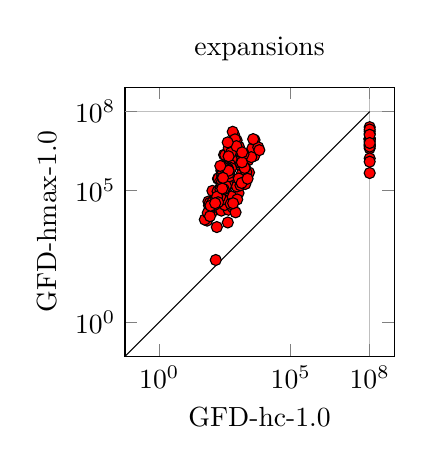
\begin{tikzpicture}
\begin{axis}[extra x tick style={grid=major}, extra x ticks=100000000, extra y tick style={grid=major}, extra y ticks=100000000, height=5cm, legend cell align=left, legend style={at=(1.3, 0.5)}, title=expansions, width=5cm, xlabel=GFD-hc-1.0, xmin=0.05, xmode=log, ylabel=GFD-hmax-1.0, ymin=0.05, ymode=log]
\addplot[color=red, mark=*, mark options={{draw=black}}, only marks] coordinates {
(230, 569769) (2591, 484804) (148, 19807) (949, 1338018) (78, 26957) (405, 1134115) (4105, 2084682) (105, 97335) (276, 239099) (245, 467887) (405, 6110) (66, 7189) (753, 1203962) (1582, 2436290) (552, 946522) (100, 15036) (3489, 4039321) (257, 722573) (890, 4678237) (100000000, 14429609) (824, 6565690) (1361, 429112) (250, 36670) (442, 238476) (1183, 942364) (406, 165460) (332, 129626) (100000000, 17564425) (122, 39369) (4197, 8304052) (97, 38739) (2377, 1398052) (982, 1212966) (444, 1895640) (2039, 503431) (1316, 223040) (54, 7863) (533, 1902459) (179, 22212) (577, 970224) (100000000, 9213922) (171, 280897) (1036, 80497) (100000000, 5447075) (155, 4085) (76, 15309) (181, 295964) (245, 192962) (1024, 4035559) (5822, 4381078) (100000000, 463156) (3719, 9011312) (318, 265061) (390, 73435) (100000000, 4039321) (463, 346481) (265, 467488) (522, 2879722) (454, 4131519) (231, 17228) (100000000, 1666945) (344, 1008929) (74, 38249) (228, 154522) (430, 18579) (84, 33663) (100000000, 25664002) (100000000, 9293025) (100000000, 20869531) (196, 75267) (214, 50407) (247, 393581) (100000000, 9003910) (446, 457505) (100000000, 1247318) (545, 59188) (469, 650417) (228, 259042) (100000000, 5313085) (565, 1591836) (1801, 762223) (226, 33750) (70, 14136) (315, 28328) (451, 1002023) (700, 13226508) (886, 3583409) (621, 17124128) (292, 2289408) (105, 35597) (100000000, 9607172) (100000000, 7296113) (141, 229) (900, 142664) (1222, 158411) (922, 45750) (1878, 177904) (604, 23892) (473, 660527) (251, 305652) (251, 77922) (491, 965177) (6395, 3436782) (277, 84151) (488, 3239978) (542, 714019) (85, 10527) (323, 2229316) (165, 93183) (442, 4141370) (344, 148709) (259, 45579) (208, 59159) (1064, 4674644) (876, 8196197) (799, 14843) (146, 47869) (100000000, 8505860) (128, 28682) (528, 2710900) (362, 759016) (1058, 286877) (212, 109366) (520, 30956) (759, 8822967) (410, 686505) (3172, 1860195) (1359, 194064) (859, 4878582) (2285, 281707) (428, 606219) (401, 6781895) (100000000, 13178141) (433, 2005643) (1600, 2410828) (100000000, 4675490) (159, 59011) (1758, 722706) (643, 32901) (1394, 1178832) (173, 35767) (89, 26398) (284, 112222) (134, 33117) (249, 118840) (430, 567474) (100000000, 6392143) (266, 303265) (1420, 2825321) (210, 862634)
};
\addplot[color=black] coordinates {(0.050000, 0.050000) (100000000, 100000000)};
\end{axis}
\end{tikzpicture}
	\end{minipage}
	\hfill
	\begin{minipage}{0.2\textwidth}
		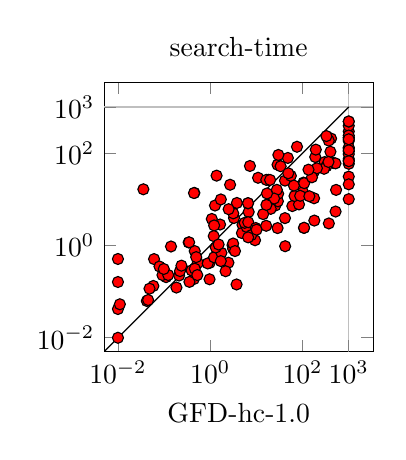
\begin{tikzpicture}
\begin{axis}[extra x tick style={grid=major}, extra x ticks=1000, extra y tick style={grid=major}, extra y ticks=1000, height=5cm, legend cell align=left, legend style={at=(1.3, 0.5)}, title=search-time, width=5cm, xlabel=GFD-hc-1.0, xmin=0.005, xmode=log, ymin=0.005, ymode=log]
\addplot[color=red, mark=*, mark options={{draw=black}}, only marks] coordinates {
(301.059000, 64.031400) (41.494500, 3.908850) (18.060000, 26.414800) (414.128000, 206.848000) (178.548000, 40.702900) (10.856300, 29.239800) (1000, 184.396000) (179.593000, 3.457570) (4.992770, 2.793460) (4.849830, 1.854280) (0.211347, 0.223396) (1000, 296.241000) (1000, 390.885000) (59.877200, 7.130300) (0.042275, 0.062697) (0.220443, 0.278667) (16.366100, 26.357100) (41.562600, 25.405900) (0.441774, 0.187157) (83.637400, 7.753840) (0.141068, 0.949125) (107.172000, 2.399890) (25.669700, 7.320520) (29.157800, 9.057790) (75.720700, 137.315000) (3.714660, 0.142928) (3.034160, 1.013160) (6.788090, 5.317440) (0.970045, 0.419907) (0.394426, 0.287559) (0.353660, 0.162390) (0.538966, 0.417593) (9.329720, 1.298190) (0.010000, 0.010000) (0.058476, 0.132549) (47.931700, 78.702700) (462.750000, 61.231700) (370.224000, 2.998630) (532.161000, 15.970100) (0.460507, 0.755070) (0.010000, 0.041957) (188.015000, 82.485700) (518.313000, 5.425410) (515.875000, 60.002000) (1000, 483.450000) (0.237329, 0.365226) (3.262710, 3.929670) (400.865000, 107.182000) (29.561600, 13.222000) (6.111430, 2.521750) (2.473950, 0.422852) (27.714000, 16.019100) (1000, 30.990100) (0.035529, 16.469100) (368.798000, 186.933000) (5.567260, 3.092950) (1.370050, 32.517600) (328.711000, 52.036000) (0.102103, 0.264352) (0.060547, 0.506678) (28.674500, 55.993400) (16.985300, 7.685750) (3.128690, 0.846171) (0.079532, 0.349770) (0.110222, 0.205991) (1.079380, 3.746840) (1000, 21.095400) (0.340022, 1.163520) (0.010000, 0.161466) (1000, 126.680000) (0.462227, 0.313519) (6.637260, 3.193290) (104.419000, 22.985800) (1000, 132.272000) (66.918400, 11.792400) (0.045021, 0.065806) (1000, 58.661300) (1.466410, 0.703081) (7.710920, 1.675180) (6.565130, 8.219100) (0.092073, 0.228503) (0.010000, 0.509048) (19.405500, 7.452050) (55.639600, 32.216100) (33.438600, 51.958700) (193.357000, 119.056000) (1000, 68.511400) (159.468000, 41.071800) (1000, 75.038400) (2.146200, 0.276449) (64.923900, 19.807400) (0.452254, 13.780200) (177.342000, 10.525300) (3.773480, 8.325430) (328.191000, 234.044000) (24.133800, 10.383100) (6.618680, 1.496810) (1.630710, 2.841840) (3.149460, 4.962510) (1.211950, 2.710900) (1000, 108.808000) (1000, 485.321000) (0.048231, 0.115710) (1.266170, 7.330720) (0.881060, 0.407789) (1.206840, 0.553831) (20.368000, 6.207500) (0.348218, 1.168290) (3.125510, 1.101390) (1000, 216.066000) (101.978000, 14.279900) (1000, 95.150700) (41.907000, 0.962452) (13.973900, 4.774420) (0.122720, 0.228868) (6.578410, 8.235650) (0.098489, 0.309166) (291.877000, 45.819300) (9.671090, 2.386450) (88.587000, 11.908900) (0.964024, 0.184939) (108.227000, 22.379100) (1000, 216.300000) (48.895200, 36.609200) (0.523978, 0.228302) (204.100000, 46.981400) (1000, 240.508000) (3.428330, 0.755814) (2.498100, 6.100800) (16.451900, 7.544050) (1.742990, 0.691586) (16.911900, 13.373300) (10.081500, 2.195440) (107.757000, 2.410660) (1.315320, 0.903194) (1000, 10.069100) (0.184853, 0.122402) (159.964000, 30.028100) (0.496160, 0.558590) (1000, 67.051300) (2.686900, 20.655100) (1.689510, 0.457708) (134.183000, 43.812500) (1000, 115.526000) (363.461000, 64.412800) (1000, 199.610000) (28.727300, 2.376690) (0.444038, 13.644000) (139.989000, 11.640200) (7.228740, 52.657100) (1.188720, 1.593310) (19.748200, 26.282800) (29.878000, 91.307800) (0.010997, 0.053189) (1.516060, 1.049650) (1.693460, 9.920000) (16.261200, 2.666230)
};
\addplot[color=black] coordinates {(0.0050000, 0.0050000) (1000, 1000)};
\end{axis}
\end{tikzpicture}
	\end{minipage}
	\caption{Comparison of expansions and search time per task (RCP domains) of $h^{max}$ and $h^C$ for bounded IPC domains}
\end{figure}





\begin{figure}[ht]
		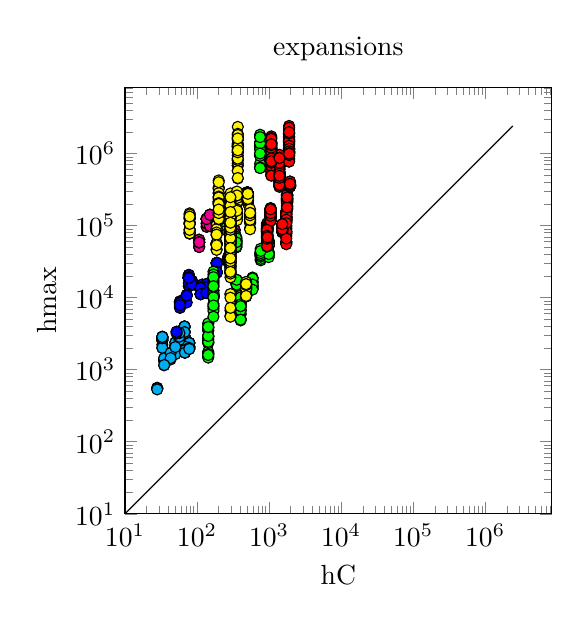
\begin{tikzpicture}
\begin{axis}[extra x tick style={grid=major}, extra x ticks=10000000, 
extra y tick style={grid=major}, extra y ticks=10000000, height=7.00cm, 
legend cell align=left, title=expansions, 
width=7.00cm, xlabel=hC, xmin=10, xmode=log, ylabel=hmax, ymin=10, ymode=log]

\addplot[color=cyan, mark=*, mark options={{draw=black}}, only marks] coordinates {
(67, 3970) (35, 1401) (67, 3372) (68, 1736) (43, 1672) (67, 3991) (28, 553) (57, 2580) (67, 3911) (57, 3216) (33, 2563) (35, 1151) (68, 2098) (68, 1860) (50, 1780) (78, 2093) (78, 2022) (50, 2159) (57, 3252) (68, 2078) (57, 2583) (28, 543) (68, 2089) (35, 1389) (78, 2107) (68, 1852) (67, 3965) (43, 1682) (78, 2345) (78, 1942) (50, 2006) (67, 3286) (78, 2355) (67, 3338) (67, 3905) (68, 2094) (68, 2105) (50, 1961) (78, 2100) (35, 1339) (67, 3365) (33, 2562) (33, 2009) (78, 2014) (50, 2055) (33, 2729) (67, 3302) (67, 3938) (50, 2392) (57, 3245) (68, 1727) (50, 2071) (68, 1859) (67, 2913) (68, 2087) (35, 1424) (68, 2079) (57, 2582) (50, 2061) (68, 1871) (67, 3317) (57, 2907) (43, 1460) (35, 1434) (50, 1771) (68, 1853) (67, 3919) (33, 2733) (68, 1868) (33, 2857) (67, 2918) (68, 1728) (33, 2866) (57, 3208) (67, 2917) (67, 2934) (78, 1950) (57, 3206) (43, 1710) (50, 1998) (33, 2737) (78, 2363) (43, 1717) (50, 1951) (33, 2561) (33, 2850) (28, 562) (35, 1332) (28, 552) (50, 2173) (78, 2356) (50, 2014) (35, 1322) (78, 2347) (35, 1391) (67, 3417) (33, 2572) (68, 2097) (50, 2384) (68, 1878) (67, 3952) (43, 1388) (78, 2006) (28, 533) (33, 2220) (35, 1441) (67, 3976) (50, 1641) (68, 1729) (33, 2015) (57, 2590) (43, 1705) (43, 1450) (50, 2064) (67, 3325) (33, 2859) (78, 1943) (57, 2874) (57, 3232) (35, 1161) (33, 2730) (33, 2849)
};
%\addlegendentry{TPP\_uc\_5M\_3G}
\addplot[color=blue, mark=*, mark options={{draw=black}}, only marks] coordinates {
(77, 19319) (112, 13687) (112, 12950) (272, 31637) (135, 15473) (135, 14109) (112, 12967) (272, 35404) (77, 18726) (58, 8424) (188, 22685) (272, 31661) (58, 8864) (72, 10748) (188, 30393) (135, 11689) (135, 13966) (272, 36712) (135, 14112) (58, 7233) (272, 35361) (112, 11222) (72, 10908) (85, 15143) (77, 18762) (135, 14071) (72, 8559) (135, 13934) (272, 32714) (85, 16992) (118, 13046) (135, 13965) (77, 14394) (112, 13655) (112, 12918) (112, 13717) (77, 18728) (112, 12980) (135, 13995) (135, 11638) (77, 19339) (58, 8449) (272, 32733) (77, 18703) (58, 7906) (188, 30382) (77, 14408) (272, 36212) (85, 15276) (52, 3182) (135, 13998) (58, 8846) (72, 10733) (118, 15181) (77, 19338) (272, 36680) (118, 12656) (112, 12951) (77, 19355) (188, 30389) (112, 11190) (77, 20679) (77, 18706) (188, 30368) (112, 11207) (188, 30366) (58, 7873) (85, 17051) (272, 32765) (112, 13623) (77, 18747) (77, 19358) (58, 7251) (77, 18708) (58, 8879) (112, 13702) (77, 19373) (188, 22379) (135, 15443) (188, 28814) (85, 15083) (72, 10926) (272, 36197) (188, 30378) (112, 13640) (77, 18727) (77, 19314) (58, 8467) (135, 14082) (77, 20664) (272, 36194) (112, 13010) (118, 11652) (188, 22703) (85, 16991) (85, 15275) (118, 15199) (77, 19317) (272, 36678) (272, 31620) (188, 22492) (112, 11191) (77, 19337) (118, 11740) (58, 7891) (77, 20629) (135, 15426) (188, 30367) (112, 12991) (135, 14049) (272, 32766) (77, 20644) (112, 12937) (272, 31636) (52, 3375) (118, 12674) (77, 18723) (272, 35422) (112, 13652) (77, 19334) (272, 35385) (77, 16027) (52, 3357) (135, 11658) (272, 35438) (272, 32734) (272, 32710) (112, 13680) (188, 22475) (85, 17052) (85, 15336) (188, 30376) (135, 13983) (188, 22171) (112, 13671) (272, 36620) (112, 11173) (77, 18744) (135, 11674) (188, 22493) (188, 30391) (188, 22701) (72, 10715)
};
%\addlegendentry{TPP\_uc\_5M\_4G}
\addplot[color=magenta, mark=*, mark options={{draw=black}}, only marks] coordinates {
(107, 58961) (151, 129354) (331, 87333) (500, 286869) (266, 138317) (293, 66651) (500, 269672) (500, 241957) (260, 107200) (222, 111655) (136, 96218) (266, 124009) (151, 98643) (151, 129310) (222, 111689) (107, 50632) (500, 269127) (222, 125930) (293, 68667) (260, 116309) (260, 116416) (222, 111751) (293, 66568) (151, 141380) (151, 134538) (107, 58636) (500, 289505) (151, 134263) (222, 119659) (500, 286759) (500, 289439) (500, 269574) (331, 78351) (500, 267648) (331, 87059) (331, 78317) (331, 87367) (260, 85833) (331, 72965) (222, 130659) (107, 63618) (500, 269204) (331, 78173) (266, 113848) (500, 269703) (500, 286844) (500, 241894) (151, 134266) (266, 117008) (266, 116919) (151, 134470) (151, 129358) (500, 267479) (136, 96760) (500, 289443) (500, 269172) (500, 267553) (151, 129321) (500, 267517) (500, 269671) (266, 113882) (151, 141449) (331, 87398) (331, 85919) (151, 98852) (222, 119596) (151, 134469) (293, 66602) (136, 123874) (151, 141418) (266, 123978) (222, 119497) (331, 73061) (500, 241863) (500, 285768) (222, 111652) (151, 129101) (500, 241901) (222, 125836) (500, 269139) (260, 101960) (151, 129148) (500, 267522) (260, 102414) (266, 132089) (266, 116888) (293, 68666) (500, 289507) (500, 286898) (500, 244306) (222, 119565) (266, 138285) (500, 269076) (107, 63553) (136, 123613) (266, 116975) (136, 125489) (260, 107327) (136, 106987) (151, 134250) (222, 119628) (222, 130690) (151, 129114) (266, 117040) (260, 102436) (331, 72931) (107, 50663) (222, 119467) (260, 86266) (266, 138286) (500, 285800) (500, 244370) (222, 125868) (260, 116540) (222, 130752) (500, 244308) (151, 129320) (500, 267518) (331, 85953) (331, 87093) (151, 111143) (266, 124041) (151, 134297) (500, 286829) (107, 58896) (222, 130625) (151, 129117) (222, 111618) (500, 289569) (260, 107313) (500, 289472) (136, 106953) (136, 125523) (266, 132058) (293, 66685) (293, 60796) (151, 129389) (151, 134507) (266, 123945) (222, 130721) (500, 269142) (500, 244305) (500, 267585) (260, 107447) (266, 113817) (293, 57171) (331, 85984) (266, 132024) (500, 285831) (266, 138254) (107, 50598) (260, 102498) (107, 58930) (293, 60762) (151, 134503) (260, 86141) (136, 123555) (500, 241891) (107, 58594) (500, 244340) (500, 285799) (151, 98882) (260, 102371) (151, 134459) (266, 113667) (222, 125773) (107, 63680) (266, 138221) (107, 58571) (266, 124010) (500, 267649) (500, 285739) (500, 269767) (107, 58593) (500, 244371) (331, 87124) (260, 102494) (151, 141348) (107, 58698) (136, 123840) (136, 123647) (500, 269637) (222, 125898) (500, 244339) (260, 86204) (500, 267587) (500, 289411) (151, 141340) (500, 286962) (222, 111720) (260, 107451) (222, 119627) (331, 78263) (500, 285765) (222, 125805) (500, 241926)
};
%\addlegendentry{TPP\_uc\_5M\_5G}
\addplot[color=green, mark=*, mark options={{draw=black}}, only marks] coordinates {
(403, 7282) (751, 1828930) (214, 114934) (169, 7554) (765, 39465) (589, 18643) (214, 126863) (403, 10149) (355, 15048) (403, 6850) (214, 128114) (143, 2346) (143, 3539) (589, 15999) (169, 10951) (143, 1517) (751, 633208) (350, 63125) (143, 1721) (765, 41818) (214, 120351) (751, 640479) (169, 16572) (751, 1002703) (751, 1284276) (403, 8290) (350, 61546) (403, 5836) (751, 1165178) (214, 122086) (403, 9120) (765, 39449) (350, 62727) (350, 61730) (169, 19066) (214, 123619) (169, 11054) (751, 1690327) (350, 58821) (751, 961118) (214, 127514) (143, 2411) (751, 725693) (350, 63568) (350, 49829) (143, 2916) (751, 643827) (214, 131745) (765, 33003) (589, 16566) (350, 55339) (350, 56954) (990, 57423) (765, 34664) (765, 41993) (990, 41518) (355, 16779) (403, 7630) (169, 22967) (751, 946492) (765, 47777) (214, 160338) (403, 11205) (169, 17370) (169, 14034) (143, 2853) (751, 1293679) (214, 135445) (990, 53910) (350, 60174) (990, 52675) (350, 65428) (169, 7080) (169, 9782) (214, 141870) (355, 16200) (403, 8258) (355, 14953) (403, 9626) (169, 8197) (350, 53494) (214, 111881) (751, 1427130) (350, 50267) (589, 18305) (765, 42759) (214, 105837) (169, 6544) (169, 20944) (751, 1432392) (403, 9219) (765, 38691) (403, 6595) (350, 54203) (403, 4982) (355, 15543) (990, 52488) (403, 6062) (355, 15605) (751, 1241372) (355, 17715) (355, 15335) (169, 10520) (765, 37295) (214, 131743) (214, 112960) (143, 4314) (765, 40416) (169, 15146) (143, 2989) (143, 4404) (403, 9159) (169, 12502) (143, 2922) (214, 140814) (403, 10168) (169, 11106) (355, 16701) (990, 40164) (350, 68006) (589, 19050) (403, 7587) (990, 40321) (589, 13115) (143, 1665) (765, 41977) (143, 3854) (214, 135704) (990, 42156) (990, 61489) (990, 41530) (751, 949401) (990, 40180) (169, 5443) (169, 12643) (214, 112962) (143, 2671) (350, 60636) (214, 140818) (350, 61878) (143, 3476) (143, 1668) (355, 16476) (143, 2575) (751, 1142746) (143, 3782) (143, 1613) (751, 934680) (355, 16406) (751, 629817) (143, 3888) (169, 10344) (990, 59959) (350, 51691) (350, 55409) (214, 105346) (403, 5078) (169, 10175) (990, 40760) (765, 42724) (589, 16447) (143, 2352) (751, 1388239) (214, 116597) (169, 15850) (143, 1785) (169, 11720) (169, 10326) (751, 1002695) (143, 2844) (589, 14001) (143, 2438) (403, 4834) (990, 59781) (355, 16829) (403, 8778) (990, 59975) (403, 8555) (350, 70160) (214, 100660) (143, 2936) (214, 112413) (589, 13603) (214, 141904) (214, 126865) (350, 59170) (169, 10550) (990, 40776) (143, 1471) (350, 65707) (350, 58161) (990, 60242) (169, 18300) (403, 6678) (990, 36548) (355, 15665) (765, 37383) (589, 16877) (143, 3897) (355, 16663) (990, 57545) (143, 1664) (214, 160336) (765, 39232) (403, 7621) (589, 14780) (990, 57407) (169, 10116) (350, 60153) (169, 19304) (350, 55910) (214, 123683) (350, 55617) (350, 51232) (990, 53878) (403, 10714) (169, 7798) (403, 9979) (589, 18502) (403, 9983) (589, 14547) (589, 13591) (403, 10070) (765, 39310) (765, 41572) (355, 15194) (143, 3922) (350, 67014) (214, 127635) (403, 8065) (990, 42837) (589, 15257) (751, 1694233) (355, 17675) (350, 51261) (350, 58652) (589, 12924) (990, 40319) (169, 14449) (403, 7626) (765, 44495) (143, 1601) (403, 4949)
};
%\addlegendentry{nomystery\_6L\_4P}
\addplot[color=yellow, mark=*, mark options={{draw=black}}, only marks] coordinates {
(508, 262363) (200, 164885) (358, 261204) (291, 11132) (79, 142194) (291, 219450) (291, 124175) (291, 88758) (508, 244448) (291, 28144) (291, 69365) (291, 94946) (291, 90937) (187, 89013) (480, 10445) (508, 221212) (291, 109991) (480, 14806) (291, 279554) (200, 245968) (291, 69215) (291, 133963) (291, 103163) (291, 72808) (291, 56602) (368, 1374599) (200, 331844) (79, 80793) (358, 155872) (291, 125458) (291, 139004) (368, 2348628) (291, 243303) (291, 41307) (291, 120601) (291, 172638) (291, 89033) (291, 61468) (291, 104019) (200, 214603) (480, 10400) (187, 56596) (358, 213341) (480, 16518) (291, 81257) (358, 141751) (291, 91654) (291, 62517) (291, 73288) (291, 114379) (79, 126812) (291, 47438) (200, 339697) (480, 14810) (545, 110458) (291, 56643) (291, 165391) (545, 92347) (291, 40996) (291, 44801) (291, 97696) (291, 126251) (480, 14854) (291, 174674) (291, 120198) (291, 11229) (79, 88453) (291, 62276) (508, 257634) (291, 98341) (291, 106977) (291, 50740) (291, 76875) (480, 13156) (358, 133359) (291, 27451) (291, 102734) (291, 34264) (545, 113116) (291, 43722) (291, 184660) (79, 106177) (200, 201758) (291, 88693) (291, 41246) (187, 92062) (291, 48438) (291, 138346) (291, 166132) (291, 159323) (291, 96742) (291, 136765) (79, 105713) (291, 62818) (291, 86391) (291, 61322) (291, 136641) (291, 33300) (291, 104245) (79, 148189) (291, 68358) (545, 146365) (368, 1336077) (291, 134117) (368, 581963) (368, 1881765) (291, 83176) (291, 111635) (291, 100167) (545, 108542) (291, 75451) (358, 133459) (508, 237521) (291, 106774) (200, 194943) (291, 109045) (291, 89183) (480, 14181) (291, 67386) (480, 13160) (291, 86491) (368, 687015) (508, 257618) (291, 146019) (291, 104630) (508, 205474) (358, 135234) (291, 23536) (291, 94149) (79, 77666) (291, 49556) (368, 1276751) (291, 43765) (291, 31387) (291, 5583) (508, 238206) (358, 146837) (291, 56789) (200, 212019) (291, 70547) (508, 283424) (358, 161467) (291, 69604) (358, 245542) (508, 248360) (291, 134396) (508, 249024) (291, 48987) (291, 68133) (291, 64793) (200, 151180) (291, 111232) (291, 86378) (545, 120891) (508, 232707) (291, 43750) (291, 147985) (187, 102179) (291, 44814) (291, 61487) (291, 95842) (291, 88406) (508, 232808) (291, 122440) (291, 69927) (291, 129699) (187, 56399) (200, 123689) (368, 1696187) (291, 55571) (291, 102471) (508, 210866) (291, 94585) (291, 151436) (291, 31477) (545, 130292) (291, 94603) (480, 11141) (79, 77671) (291, 122956) (480, 14975) (291, 136406) (187, 88018) (508, 237513) (187, 89434) (291, 132841) (291, 30449) (291, 115590) (291, 189178) (291, 91906) (368, 1040472) (291, 134124) (368, 679689) (291, 101143) (200, 424811) (291, 68171) (79, 142378) (508, 205466) (291, 84196) (200, 165100) (358, 206443) (291, 23223) (291, 40427) (291, 126226) (291, 24784) (358, 146865) (291, 6660) (291, 79598) (200, 122809) (79, 110684) (291, 77553) (187, 56590) (291, 69079) (358, 205347) (291, 91197) (480, 10435) (291, 100113) (200, 282938) (291, 119960) (291, 140130) (291, 132099) (368, 734500) (187, 46602) (79, 131364) (368, 937395) (200, 212080) (508, 223056) (368, 814838) (291, 135334) (291, 5447) (545, 89088) (291, 72398) (358, 138724) (291, 197241) (200, 141164) (291, 113632) (291, 185821) (291, 131947) (358, 146942) (291, 22649) (291, 32179) (291, 104076) (200, 235620) (291, 132641) (200, 323658) (291, 94485) (545, 119397) (291, 49714) (358, 121712) (545, 135894) (291, 108865) (291, 126868) (358, 241781) (291, 159347) (291, 160324) (291, 104603) (291, 42424) (291, 78799) (291, 134326) (200, 282900) (79, 126952) (291, 22054) (291, 155473) (291, 36266) (368, 853383) (291, 173701) (368, 574633) (358, 118654) (480, 13713) (187, 54641) (291, 49971) (291, 79773) (291, 112369) (291, 143397) (291, 19138) (368, 1546116) (368, 813854) (368, 1276823) (480, 10892) (291, 84285) (187, 80329) (200, 253498) (368, 1236848) (79, 123874) (291, 100896) (291, 42634) (291, 108951) (291, 37225) (291, 99827) (291, 36807) (291, 131524) (291, 110618) (200, 217124) (291, 45219) (291, 91456) (508, 276170) (291, 180200) (291, 126684) (291, 135216) (291, 95386) (291, 68452) (200, 245913) (291, 77846) (508, 221833) (291, 130911) (480, 14018) (291, 36773) (291, 53775) (358, 262589) (368, 1625092) (291, 165376) (508, 250736) (200, 205749) (187, 46086) (508, 223048) (291, 9983) (291, 70556) (291, 22417) (79, 87098) (291, 140258) (291, 161849) (368, 451011) (291, 101360) (200, 400531) (291, 156905) (291, 40632) (291, 88870) (291, 35197) (291, 180144) (291, 124527) (291, 96150) (480, 16516) (508, 283432) (291, 61436) (291, 65540) (291, 38491) (79, 110682) (291, 201103) (480, 14032) (291, 88348) (368, 458169) (291, 112348) (291, 32017) (291, 170799) (79, 80788) (480, 11118) (368, 1070088) (545, 130986) (508, 221327) (545, 120195) (291, 114438) (291, 150877) (291, 91313) (291, 164579) (291, 63040) (508, 250314) (291, 99721) (291, 163120) (291, 58183) (79, 78032) (291, 94754) (358, 297586) (291, 83596) (508, 248222) (545, 138993) (79, 106172) (291, 134953) (291, 21584) (200, 141187) (291, 90673) (291, 158902) (291, 123597) (291, 152320) (79, 87103) (291, 70655) (291, 107676) (358, 168152) (358, 138719) (291, 92197) (368, 1144025) (480, 15400) (368, 853389) (291, 129487) (291, 137101) (291, 46528) (291, 51977) (291, 71571) (291, 130086) (200, 123068) (291, 88645) (291, 81979) (358, 262593) (291, 224852) (368, 1041717) (291, 139571) (480, 13188) (291, 69306) (291, 78479) (291, 30336) (291, 70750) (291, 27007) (291, 87986) (291, 35356) (291, 44774) (291, 111495) (291, 109307) (291, 39983) (291, 96866) (291, 112247) (291, 70794) (368, 1814237) (291, 7221) (291, 26516) (291, 106345) (508, 219361) (291, 118365) (480, 13667) (291, 108853) (480, 14850) (480, 10582) (291, 31670) (291, 86423) (291, 139467) (291, 82206) (187, 55121) (291, 133637) (79, 105708) (291, 213728) (291, 29044) (291, 37194) (187, 55085) (291, 148831) (187, 74314) (291, 73769) (291, 89267) (291, 113350) (200, 123930) (291, 93485) (291, 47387) (480, 10879) (368, 1236852) (291, 33692) (480, 13192) (291, 93838) (291, 25519) (291, 94851) (291, 100566) (508, 227498) (291, 38548) (291, 199605) (291, 124382) (291, 30173) (291, 32068) (291, 57974) (291, 128426) (291, 136717) (480, 14983) (200, 200124) (291, 151578) (368, 1625164) (291, 141561) (480, 15412) (200, 149440) (291, 129298) (291, 116649) (291, 117299) (187, 57157) (291, 189799) (358, 160945) (291, 76337) (291, 102937) (291, 247980) (545, 169125) (291, 128416) (368, 1110471) (508, 235288) (508, 276161) (187, 75000) (291, 154487) (545, 149008) (291, 74772) (291, 22837) (480, 10577) (291, 67260) (200, 167474) (291, 89415) (79, 133694) (291, 35099) (291, 101740) (291, 87565) (545, 150097) (291, 93928) (291, 109734) (187, 53407) (291, 48901)
};
%\addlegendentry{nomystery\_6L\_4P\_c120}
\addplot[color=red, mark=*, mark options={{draw=black}}, only marks] coordinates {
(1734, 92280) (1050, 165371) (1896, 1389644) (1074, 1737339) (1734, 146721) (1779, 243300) (1734, 118784) (938, 87566) (1734, 134006) (1529, 102133) (1050, 139234) (1951, 352800) (1074, 683092) (1734, 114141) (1529, 91922) (953, 66419) (1734, 116464) (1393, 449570) (1050, 117616) (1896, 1317573) (953, 57112) (1074, 715777) (938, 56639) (1393, 710119) (1529, 96536) (1050, 132150) (1393, 513173) (1951, 352333) (1734, 76631) (1896, 1693586) (1050, 146061) (1050, 148972) (1779, 239880) (1074, 558947) (1074, 974508) (1779, 234884) (1529, 101074) (1734, 112537) (1393, 862522) (1050, 145432) (1393, 716709) (1074, 1200526) (1779, 187278) (1529, 103252) (1779, 268366) (1074, 890977) (1896, 1001924) (1074, 1165056) (938, 90890) (1074, 1118937) (938, 85144) (1393, 497195) (938, 84220) (1779, 265474) (1074, 678578) (1779, 170944) (1074, 884938) (1734, 154427) (938, 79111) (1050, 150558) (1529, 85122) (1393, 460580) (1074, 1421674) (1896, 1133273) (1529, 93021) (1393, 535687) (1393, 602037) (1393, 660227) (1050, 164779) (1896, 1468956) (1050, 117106) (1896, 1738809) (1074, 514733) (1896, 1040204) (1529, 91890) (1074, 1165087) (1779, 213507) (1074, 974482) (1074, 1374431) (1734, 131567) (1050, 175290) (1074, 710830) (1951, 367312) (1896, 855103) (1779, 254543) (1393, 600086) (1734, 132365) (1896, 953968) (1529, 88169) (1734, 154597) (1951, 349672) (1779, 268339) (1050, 151457) (938, 70895) (1074, 1023846) (1074, 514535) (938, 51165) (1393, 710161) (1074, 716087) (1529, 102109) (1529, 82942) (1050, 161207) (1393, 750624) (1951, 362053) (1779, 235426) (1393, 759060) (1734, 127188) (938, 91572) (1779, 222503) (1779, 172876) (1529, 86595) (1074, 828779) (1951, 379516) (953, 66365) (1050, 137562) (1074, 1123653) (1529, 90618) (1529, 92416) (1896, 1423432) (1734, 132247) (1896, 1013202) (1896, 2153383) (1393, 527127) (1050, 134055) (953, 58958) (953, 94652) (1734, 59429) (1779, 179418) (953, 89376) (1779, 265644) (1074, 926719) (1779, 233578) (1896, 1189284) (1393, 541938) (1734, 121192) (1896, 1050238) (1393, 542073) (953, 63382) (1779, 216350) (938, 104642) (953, 94449) (938, 83153) (938, 89158) (938, 83361) (1896, 1913780) (1074, 1346407) (1050, 130120) (1896, 2271627) (1074, 762506) (1896, 1168398) (1529, 96095) (1074, 1425049) (1734, 120478) (1529, 83072) (938, 98907) (1734, 108805) (938, 59266) (1779, 227826) (1896, 997558) (1050, 142918) (1393, 524203) (1951, 365946) (953, 66119) (1896, 1049043) (1951, 354498) (1050, 137005) (938, 92086) (1393, 550404) (1050, 154868) (1779, 235024) (1050, 156935) (1393, 506124) (938, 96303) (1393, 963976) (1529, 103268) (1074, 1448962) (1074, 991389) (1074, 801370) (938, 52270) (1529, 90958) (1951, 409474) (1529, 90786) (1050, 117680) (1393, 540623) (1050, 149139) (1779, 268341) (1393, 400499) (953, 107647) (1779, 259024) (1734, 156255) (953, 59032) (953, 66189) (1050, 170341) (1779, 171395) (1050, 147111) (1050, 173005) (938, 107644) (1734, 145171) (1529, 90891) (1529, 98289) (1529, 82918) (1734, 59902) (1393, 349595) (1896, 1063449) (1529, 86699) (1779, 227814) (1734, 77958) (938, 83596) (1529, 80912) (1951, 376628) (1529, 96616) (1393, 500283) (1951, 354570) (938, 100456) (1393, 499208) (1393, 705053) (1074, 738218) (953, 91212) (1393, 676856) (938, 60411) (1074, 1228841) (1393, 834900) (1050, 136211) (1393, 400638) (1050, 153763) (1529, 88185) (1074, 1375025) (1779, 183224) (1529, 96077) (1050, 135824) (1779, 211934) (1529, 90602) (1074, 996647) (1393, 399014) (1050, 152914) (1734, 123061) (1074, 711578) (1393, 464162) (1529, 101090) (1734, 98222) (1050, 149615) (1393, 753701) (1529, 86611) (1393, 408862) (1779, 183195) (1050, 144575) (1951, 398490) (1734, 71350) (1050, 139797) (1779, 239081) (1393, 524201) (1529, 84068) (1734, 78822) (1050, 134368) (1951, 371057) (1779, 173327) (1074, 495494) (953, 73954) (1393, 519056) (1529, 100700) (1393, 545295) (1074, 678999) (1896, 1725251) (1529, 90910) (1050, 139382) (1050, 136588) (1951, 354164) (1074, 1284149) (1529, 82966) (1529, 101114) (1734, 82887) (1393, 367977) (1896, 1490092) (1896, 1350976) (1050, 128899) (1074, 584509) (1393, 492867) (1779, 224172) (1734, 82061) (1393, 795575) (1779, 243306) (1896, 1164016) (1896, 2422298) (1050, 148568) (1779, 259026) (938, 86986) (1529, 95128) (1529, 101843) (938, 99123) (1050, 133084) (938, 64184) (1779, 210208) (1779, 231626) (1779, 231251) (1779, 206472) (1529, 83088) (1529, 89119) (1734, 59179) (1896, 854452) (1734, 132483) (1734, 101047) (1779, 225955) (1050, 150576) (1529, 92099) (1393, 470777) (1529, 90672) (1951, 364328) (938, 95597) (1393, 451129) (1734, 127884) (1779, 259009) (1779, 168244) (1074, 1646965) (938, 79550) (1896, 1198935) (1050, 134263) (1779, 259047) (1529, 88115) (1074, 678907) (938, 85653) (1896, 815410) (1529, 103284) (1896, 1048156) (953, 60680) (938, 68022) (1529, 92400) (1074, 738316) (1529, 83224) (1779, 214820) (1779, 206853) (1050, 140360) (1074, 759122) (1050, 129382) (1050, 156161) (1393, 488736) (1734, 124511) (953, 60620) (1393, 705393) (953, 83949) (1050, 169970) (1529, 92139) (1393, 467005) (1393, 488410) (1050, 143205) (1050, 151601) (1896, 1482801) (1896, 1530640) (1896, 1127141) (1896, 1595906) (1779, 265487) (1074, 956645) (1779, 269585) (1529, 84044) (1734, 143065) (938, 96046) (1393, 627172) (1074, 860009) (1074, 787923) (1074, 747422) (1050, 128396) (1734, 89134) (1896, 1454955) (1779, 223791) (1734, 81996) (1050, 143212) (1393, 544230) (1529, 84196) (938, 81103) (1529, 88321) (1050, 144175) (1529, 102141) (1529, 95697) (1050, 149229) (1529, 90316) (1896, 1162929) (1734, 83300) (1896, 1892819) (1050, 117602) (1779, 268318) (1074, 885225) (1393, 364240) (1393, 656302) (1050, 131852) (1779, 203827) (1951, 354096) (1529, 100716) (1779, 238456) (1050, 164081) (1074, 956727) (1050, 150645) (953, 63436) (1393, 345682) (1050, 171800) (1050, 117184) (1896, 1086986) (1951, 353462) (1779, 187523) (1951, 365004) (1529, 101859) (938, 82723) (1896, 1050265) (938, 79055) (1734, 126557) (938, 68714) (1074, 682511) (1050, 133078) (1074, 678779) (1074, 771389) (1529, 90824) (953, 89367) (1529, 85130) (953, 66173) (1050, 138240) (1050, 144125) (1779, 240206) (938, 73996) (1779, 190019) (1074, 1123659) (1393, 497188) (1074, 859917) (1529, 102157) (1896, 1030518) (1734, 56330) (1074, 824970) (1393, 399147) (1393, 471881) (1393, 451005) (938, 61293) (1779, 265664) (1951, 356208) (1074, 1112698) (1896, 1579891) (953, 60674) (1734, 157210) (1896, 1499299) (1050, 149851) (1734, 123144) (938, 69382) (1896, 1285482) (1779, 222830) (1529, 88155) (1050, 159211) (1779, 253111) (1734, 55155) (1393, 467943) (1074, 828719) (953, 66425) (1050, 166437) (1529, 80872) (1074, 1102100) (1779, 268190) (1050, 139860) (1951, 348411) (1896, 925686) (1393, 364320) (938, 91590) (938, 87375) (1896, 1077148) (1896, 1920337) (938, 67040) (1896, 951363) (938, 95888) (1779, 213882) (953, 94287) (1050, 145941) (1896, 1918057) (1896, 1918792) (1529, 90508) (1393, 495920) (1050, 146703) (1951, 351531) (1896, 1030454) (1393, 551979) (1074, 1165040) (1393, 686041) (1074, 1102002) (938, 91735) (1393, 682710) (953, 69110) (1779, 232146) (1529, 103236) (1734, 140422) (1529, 85082) (1734, 149467) (1529, 95713) (1951, 362402) (1779, 213962) (1074, 1275875) (1393, 499229) (953, 57186) (1896, 1156400) (1896, 1167332) (1074, 991191) (938, 73160) (1734, 131146) (1896, 815436) (1734, 143903) (938, 89554) (1896, 2279762) (1896, 907004) (938, 51831) (1074, 495720) (1951, 356128) (1074, 854356) (1951, 369756) (1734, 66272) (953, 73934) (1896, 1077084) (1393, 743446) (1050, 138797) (1951, 371253) (1529, 95849) (953, 88240) (1074, 824378) (1529, 90688) (1050, 143364) (1050, 149389) (1734, 141402) (1074, 758583) (1074, 996871) (1393, 875433) (1529, 95160) (1896, 1013153) (1393, 488739) (938, 78203) (1896, 775718) (1050, 116978) (1734, 116626) (1074, 1204536) (1074, 1389787) (1529, 98297) (1050, 136450) (1050, 148479) (938, 80437) (938, 65829) (938, 72545) (1529, 101058) (1393, 496014) (1393, 408880) (1393, 464228) (1951, 409308) (1074, 747520) (938, 87492) (1779, 239101) (1529, 100724) (1951, 348415) (1393, 522390) (1951, 362964) (1074, 1307219) (1896, 775237) (1050, 168431) (1074, 762422) (1951, 377330) (1393, 367877) (1896, 1987957) (1951, 380462) (1734, 121002) (1896, 953631) (1393, 460479) (1779, 179042) (1074, 854678) (1393, 527575) (938, 72375) (1393, 491342) (1529, 92552) (1529, 89079) (1074, 787895) (1734, 108218) (1779, 247024) (1393, 867488) (1074, 1605594) (1074, 1349478) (953, 69108) (1529, 104840) (1896, 997253)
};
%\addlegendentry{nomystery\_6L\_5P}
\addplot[color=black] coordinates {(0.050000, 0.050000) (2422298, 2422298)};
\end{axis}
\end{tikzpicture}


		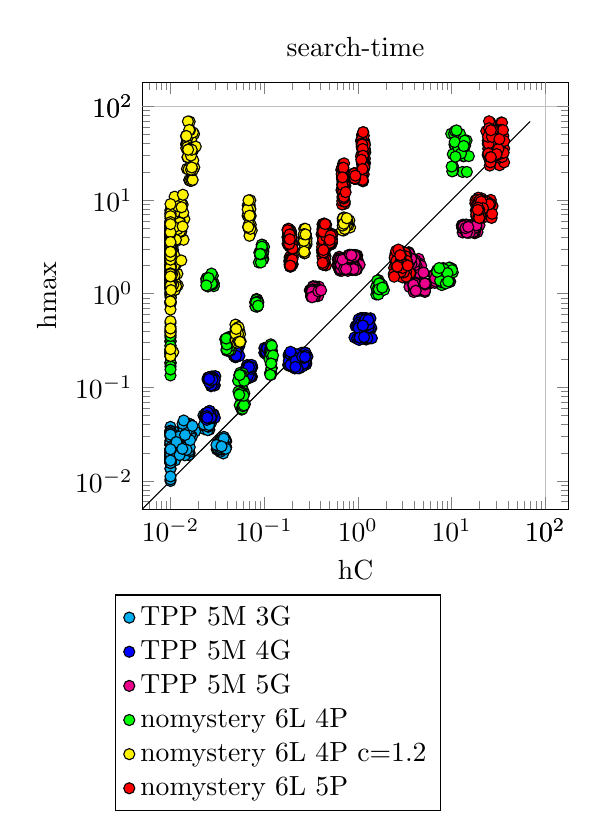
\begin{tikzpicture}
\begin{axis}[extra x tick style={grid=major}, extra x ticks=100, extra y tick style={grid=major}, 
	extra y ticks=100, height=7.00cm, legend cell align=left, legend style={at={(0.7, -0.2)}}, 
title=search-time, width=7.00cm, xlabel=hC, xmin=0.005, xmode=log, ylabel=hmax, ymin=0.005, ymode=log]
\addplot[color=cyan, mark=*, mark options={{draw=black}}, only marks] coordinates {
(0.039320, 0.026582) (0.010000, 0.032484) (0.036521, 0.025746) (0.035485, 0.020448) (0.010000, 0.013446) (0.010000, 0.020751) (0.013848, 0.030976) (0.010000, 0.020067) (0.010000, 0.024350) (0.036741, 0.024163) (0.014049, 0.023399) (0.010000, 0.015812) (0.012964, 0.023072) (0.010000, 0.026892) (0.010000, 0.018352) (0.010000, 0.020831) (0.010000, 0.024515) (0.010000, 0.020022) (0.010000, 0.019188) (0.025992, 0.035304) (0.034190, 0.020444) (0.011411, 0.024201) (0.010000, 0.020026) (0.039304, 0.022848) (0.012861, 0.022806) (0.010799, 0.033889) (0.035740, 0.027550) (0.013474, 0.026392) (0.035556, 0.024679) (0.036837, 0.020479) (0.013357, 0.022076) (0.016628, 0.037957) (0.013892, 0.029870) (0.034850, 0.027424) (0.036388, 0.025369) (0.011681, 0.021374) (0.015969, 0.019655) (0.031897, 0.025208) (0.010000, 0.025397) (0.036378, 0.021955) (0.010000, 0.016417) (0.010000, 0.017225) (0.014486, 0.022613) (0.023954, 0.039809) (0.014572, 0.021661) (0.023197, 0.035658) (0.010000, 0.032975) (0.010000, 0.019490) (0.013095, 0.019460) (0.010000, 0.026771) (0.013719, 0.034250) (0.018304, 0.033775) (0.024329, 0.039664) (0.035308, 0.024352) (0.032202, 0.021884) (0.038666, 0.027747) (0.037949, 0.027262) (0.015141, 0.032722) (0.024107, 0.047266) (0.032520, 0.022260) (0.013372, 0.020279) (0.016233, 0.040389) (0.011455, 0.022818) (0.025247, 0.045197) (0.036578, 0.019660) (0.010000, 0.018276) (0.013930, 0.022840) (0.010973, 0.017153) (0.015544, 0.020093) (0.010000, 0.034605) (0.010000, 0.017036) (0.010000, 0.010000) (0.013898, 0.022775) (0.034124, 0.027461) (0.010000, 0.021560) (0.010000, 0.037827) (0.015216, 0.024508) (0.012944, 0.022999) (0.038519, 0.027265) (0.024897, 0.047293) (0.010000, 0.024319) (0.025787, 0.040857) (0.024448, 0.040487) (0.015096, 0.025540) (0.039145, 0.022784) (0.025518, 0.039438) (0.013688, 0.024281) (0.011220, 0.016580) (0.034254, 0.025433) (0.023381, 0.038304) (0.011345, 0.029576) (0.035179, 0.022110) (0.010000, 0.019419) (0.014790, 0.033018) (0.015640, 0.018896) (0.023135, 0.040402) (0.033650, 0.026676) (0.025690, 0.039046) (0.010000, 0.032050) (0.015712, 0.038127) (0.013362, 0.030947) (0.010000, 0.033083) (0.010000, 0.017761) (0.010000, 0.020111) (0.010000, 0.032450) (0.010000, 0.016572) (0.013026, 0.025696) (0.015885, 0.020342) (0.010000, 0.018249) (0.013198, 0.020438) (0.015501, 0.039953) (0.025989, 0.048086) (0.015478, 0.023756) (0.014236, 0.039427) (0.010000, 0.034280) (0.010000, 0.016058) (0.036157, 0.025941) (0.025097, 0.046767) (0.010000, 0.018332) (0.010000, 0.024312) (0.010000, 0.020136) (0.012433, 0.026611) (0.010565, 0.021922) (0.012836, 0.026955) (0.010000, 0.015518) (0.027316, 0.042339) (0.010000, 0.034354) (0.031760, 0.024660) (0.012826, 0.024143) (0.012911, 0.020411) (0.010000, 0.031206) (0.010000, 0.025683) (0.035157, 0.027080) (0.015067, 0.030758) (0.013316, 0.019665) (0.013267, 0.020599) (0.035180, 0.024368) (0.015141, 0.027781) (0.010000, 0.032031) (0.024484, 0.039627) (0.010000, 0.030444) (0.010000, 0.020645) (0.013867, 0.025193) (0.026616, 0.050283) (0.024979, 0.034910) (0.022488, 0.050167) (0.023142, 0.047658) (0.010000, 0.018862) (0.035497, 0.024624) (0.026436, 0.045273) (0.031189, 0.021792) (0.013629, 0.039074) (0.014531, 0.041234) (0.013176, 0.026821) (0.035075, 0.021937) (0.034773, 0.023659) (0.033856, 0.023803) (0.010000, 0.019631) (0.010000, 0.017134) (0.013918, 0.037837) (0.036378, 0.022835) (0.014813, 0.037144) (0.015670, 0.023488) (0.010000, 0.033963) (0.010000, 0.017509) (0.037209, 0.029575) (0.036131, 0.025600) (0.023390, 0.046881) (0.010000, 0.016908) (0.010000, 0.030691) (0.016946, 0.029861) (0.014505, 0.038756) (0.036884, 0.022733) (0.010000, 0.019190) (0.010000, 0.021724) (0.025502, 0.039582) (0.015898, 0.040794) (0.033926, 0.020507) (0.010000, 0.033894) (0.010000, 0.018890) (0.010000, 0.032523) (0.010000, 0.013605) (0.010000, 0.021818) (0.010016, 0.018217) (0.014226, 0.018808) (0.035071, 0.026434) (0.035273, 0.022839) (0.016202, 0.030874) (0.014623, 0.034085) (0.010000, 0.015678) (0.034656, 0.023777) (0.015472, 0.022957) (0.010000, 0.016308) (0.010000, 0.032411) (0.035057, 0.021608) (0.010000, 0.020067) (0.011546, 0.028893) (0.024456, 0.052430) (0.024864, 0.047769) (0.011824, 0.029058) (0.010000, 0.015788) (0.015645, 0.039487) (0.010000, 0.017123) (0.010000, 0.019883) (0.010000, 0.015499) (0.011577, 0.025425) (0.010000, 0.030580) (0.014368, 0.026862) (0.010000, 0.031260) (0.036821, 0.024549) (0.032168, 0.021402) (0.036361, 0.023543) (0.013676, 0.027347) (0.010000, 0.030783) (0.010000, 0.019668) (0.012015, 0.025519) (0.012689, 0.020289) (0.025452, 0.037978) (0.035942, 0.025986) (0.010000, 0.010412) (0.010000, 0.022050) (0.012863, 0.020298) (0.010000, 0.029485) (0.016042, 0.035482) (0.014353, 0.027875) (0.010000, 0.011172) (0.013863, 0.034963) (0.038715, 0.023581) (0.033540, 0.021854) (0.024982, 0.038260) (0.034072, 0.023468) (0.015709, 0.038881) (0.010000, 0.019245) (0.011997, 0.024177) (0.013137, 0.023424) (0.032191, 0.022117) (0.015025, 0.034395) (0.010000, 0.016239) (0.010000, 0.018556) (0.013462, 0.040840) (0.035744, 0.022010) (0.010000, 0.015582) (0.014654, 0.022869) (0.022834, 0.040164) (0.037147, 0.024324) (0.010000, 0.019651) (0.015731, 0.021093) (0.011440, 0.027018) (0.011728, 0.027597) (0.016048, 0.022977) (0.035185, 0.027415) (0.025748, 0.039659) (0.033691, 0.022060) (0.037022, 0.028368) (0.016160, 0.027257) (0.034513, 0.022737) (0.013843, 0.044266) (0.011922, 0.024142) (0.012515, 0.018928) (0.012394, 0.029812) (0.010000, 0.031284) (0.014867, 0.021502) (0.017145, 0.038742) (0.010186, 0.023028) (0.010000, 0.021896) (0.011567, 0.026033) (0.038982, 0.022086) (0.030937, 0.024276) (0.010000, 0.021812) (0.014294, 0.030995) (0.013387, 0.022058) (0.010000, 0.016531) (0.035086, 0.023429)
};
\addlegendentry{TPP 5M 3G}
\addplot[color=blue, mark=*, mark options={{draw=black}}, only marks] coordinates {
(0.050297, 0.279710) (1.263040, 0.428969) (0.255065, 0.178802) (0.187454, 0.174292) (0.050410, 0.275998) (0.250513, 0.213799) (0.115141, 0.235412) (0.280534, 0.182792) (0.105162, 0.238285) (0.209894, 0.170831) (1.079980, 0.494964) (0.185610, 0.194387) (0.026310, 0.118275) (0.053019, 0.217491) (0.214548, 0.170996) (1.177750, 0.549168) (0.049462, 0.242973) (0.064994, 0.165661) (1.015120, 0.330901) (0.050308, 0.286648) (1.165740, 0.533976) (0.026813, 0.047981) (1.124140, 0.448465) (0.028777, 0.122090) (0.111518, 0.253040) (0.266380, 0.234697) (0.219542, 0.209512) (1.124490, 0.452618) (0.025785, 0.121586) (0.065795, 0.168199) (0.069694, 0.128647) (0.029243, 0.128211) (1.324980, 0.447141) (0.052794, 0.278175) (1.311040, 0.490320) (0.026439, 0.051147) (0.234241, 0.202623) (0.069717, 0.158753) (1.033790, 0.425113) (0.026797, 0.118192) (0.050764, 0.219772) (0.029152, 0.105985) (0.069349, 0.169650) (1.220550, 0.335203) (0.233818, 0.165618) (0.050780, 0.288135) (0.964626, 0.340255) (0.195237, 0.218255) (0.250504, 0.213707) (0.068445, 0.159292) (1.178690, 0.497507) (0.289329, 0.212968) (0.073249, 0.164960) (0.183634, 0.223248) (0.100295, 0.234358) (1.301160, 0.341540) (0.209239, 0.187751) (0.069816, 0.159747) (1.125900, 0.538630) (1.062820, 0.531859) (0.188314, 0.196133) (0.230316, 0.190312) (0.028974, 0.051449) (0.191877, 0.214966) (0.190892, 0.189553) (0.114864, 0.236737) (0.074055, 0.164773) (0.051553, 0.289763) (0.071201, 0.164349) (0.068736, 0.125609) (0.264807, 0.177577) (0.192726, 0.222720) (0.946460, 0.450036) (0.025389, 0.052708) (0.050363, 0.279397) (0.193535, 0.224637) (0.024029, 0.049666) (1.391680, 0.428189) (0.024864, 0.121252) (0.211865, 0.159134) (0.051724, 0.295699) (0.047692, 0.219688) (1.036910, 0.454470) (0.069301, 0.127901) (0.025929, 0.121386) (0.261195, 0.178750) (0.257881, 0.210760) (0.199566, 0.168665) (0.180355, 0.173772) (0.261608, 0.180421) (1.376870, 0.440359) (0.202772, 0.189774) (0.028099, 0.050966) (0.250173, 0.226796) (0.025558, 0.125160) (0.111763, 0.266859) (0.023566, 0.046992) (0.223539, 0.165644) (1.071980, 0.535234) (1.164500, 0.497985) (0.025277, 0.122099) (0.028323, 0.114633) (0.026275, 0.050830) (1.087570, 0.495403) (0.275206, 0.206685) (0.028577, 0.124552) (0.072033, 0.129052) (0.067192, 0.165408) (0.187033, 0.175110) (0.102692, 0.264521) (0.066053, 0.124183) (0.074034, 0.129750) (1.128420, 0.546528) (0.196991, 0.180998) (0.070075, 0.128319) (0.264473, 0.177471) (0.108519, 0.234397) (0.219557, 0.193199) (1.237840, 0.471433) (1.192240, 0.493862) (0.068504, 0.170328) (0.069335, 0.132783) (0.053766, 0.278249) (0.114330, 0.233378) (0.054091, 0.274177) (0.025645, 0.115693) (0.234841, 0.203505) (0.182939, 0.223370) (0.024891, 0.050778) (0.029348, 0.105420) (0.185215, 0.169508) (1.223520, 0.324194) (0.025444, 0.127747) (1.308610, 0.340428) (0.263385, 0.203788) (0.047635, 0.279715) (0.205252, 0.165934) (0.221796, 0.195594) (0.192404, 0.176427) (1.050970, 0.334608) (1.129890, 0.533476) (1.230940, 0.546208) (1.093090, 0.449748) (0.066439, 0.164789) (1.231150, 0.454687) (0.068431, 0.165871) (0.073836, 0.167315) (0.114803, 0.235980) (0.028803, 0.125272) (0.052225, 0.218157) (0.985189, 0.454264) (1.110510, 0.412662) (1.192570, 0.544124) (0.112073, 0.234903) (0.191200, 0.186275) (0.237107, 0.159666) (0.028621, 0.130453) (0.029599, 0.105483) (0.280623, 0.180699) (1.192890, 0.491793) (0.106578, 0.228409) (0.070083, 0.129055) (0.047053, 0.314009) (0.024839, 0.047244) (0.052644, 0.289475) (0.029115, 0.117777) (0.189512, 0.222692) (0.221826, 0.165929) (0.069939, 0.166272) (0.231532, 0.200403) (1.040200, 0.441260) (0.189497, 0.191068) (0.025298, 0.051290) (0.069819, 0.168472) (0.218957, 0.205723) (1.006330, 0.451174) (0.049242, 0.277687) (0.249568, 0.213594) (0.275451, 0.212184) (1.341680, 0.531891) (0.072961, 0.130412) (0.024365, 0.051256) (1.075770, 0.527259) (1.183360, 0.535480) (0.047684, 0.278937) (0.111577, 0.227300) (1.277020, 0.534342) (0.053169, 0.289024) (0.114302, 0.236840) (0.067008, 0.163449) (0.193838, 0.175796) (0.023721, 0.052787) (0.270879, 0.232024) (0.050817, 0.211515) (0.192973, 0.173296) (0.023579, 0.048078) (0.069153, 0.167464) (0.111779, 0.234648) (0.275905, 0.215341) (1.080970, 0.429990) (0.205513, 0.226570) (0.201271, 0.193362) (0.049855, 0.303960) (0.212389, 0.168926) (1.352240, 0.333734) (0.025077, 0.053894) (0.251263, 0.234038) (0.273033, 0.232651) (0.183874, 0.172520) (0.025888, 0.122122) (0.051459, 0.276620) (0.263808, 0.214122) (0.217657, 0.190464) (0.271350, 0.181718) (0.029391, 0.122101) (0.255819, 0.171728) (0.190732, 0.193776) (0.106890, 0.236294) (0.207982, 0.197656) (0.249952, 0.216466) (0.192708, 0.171711) (1.270790, 0.536287) (0.108552, 0.265799) (0.047908, 0.312841) (0.050766, 0.280320) (0.108523, 0.236667) (1.084910, 0.424003) (1.099760, 0.473859) (0.216273, 0.202783) (0.050912, 0.241751) (0.215722, 0.165670) (0.113227, 0.227268) (0.065366, 0.165401) (0.213933, 0.202266) (0.050597, 0.241581) (0.262739, 0.212464) (0.192343, 0.196671) (0.071563, 0.164856) (0.065696, 0.172841) (0.258692, 0.206896) (0.024590, 0.050966) (0.023765, 0.050899) (0.280234, 0.175356) (1.190370, 0.508558) (0.029593, 0.104887) (0.264522, 0.211360) (0.072809, 0.169141) (0.030113, 0.131691) (0.196368, 0.174199) (0.049116, 0.209639) (0.216842, 0.206658) (0.072267, 0.130954) (0.065794, 0.164627) (0.024635, 0.051079) (0.026183, 0.051170) (0.252916, 0.211061) (0.025837, 0.123817) (0.109526, 0.263921) (0.027790, 0.121338) (0.051114, 0.218380) (0.026230, 0.119012) (0.023937, 0.050238) (0.208026, 0.166816) (0.106758, 0.237245) (0.028199, 0.121564) (0.050482, 0.218206) (0.025946, 0.047401) (0.025188, 0.050649) (0.112121, 0.235670) (0.182998, 0.214940) (0.024330, 0.050111) (0.071402, 0.163374) (0.026993, 0.051068) (0.255596, 0.217434) (1.330090, 0.533883) (0.026299, 0.122271) (0.107761, 0.234410) (0.024997, 0.125838) (0.026579, 0.049684) (0.199138, 0.173356) (0.026508, 0.122753) (1.150210, 0.343476) (0.023723, 0.047088) (0.244526, 0.218547) (0.233229, 0.205531) (0.049724, 0.245760) (0.026932, 0.115768) (0.025487, 0.127720) (0.200537, 0.191152) (0.106188, 0.239684) (0.219214, 0.194679) (0.050566, 0.288757) (0.216795, 0.199887) (0.237430, 0.196414) (0.107733, 0.239795) (0.999935, 0.337100) (0.028607, 0.115511) (1.099740, 0.477789) (1.075420, 0.544188) (1.410320, 0.334475) (1.323760, 0.517789) (0.023810, 0.047128) (0.024292, 0.053234) (0.073554, 0.168842) (0.107370, 0.234986) (0.027461, 0.050441) (1.057950, 0.507466) (0.256810, 0.211752) (0.200714, 0.228286) (0.989924, 0.449727) (0.071205, 0.131214) (1.090440, 0.546863) (0.027791, 0.122762) (0.265158, 0.178706) (0.108537, 0.262320) (0.108253, 0.234688) (0.047274, 0.234691) (0.047259, 0.218837) (0.027457, 0.130656) (0.070712, 0.130607) (0.105249, 0.263538) (0.027584, 0.122636) (1.293180, 0.493534) (0.214790, 0.203698) (0.283590, 0.215476) (0.253005, 0.183599) (0.278291, 0.213472) (1.167350, 0.532917) (0.104752, 0.226913) (0.108355, 0.235860) (0.241297, 0.166468) (1.053490, 0.339236) (0.275516, 0.234760) (1.168590, 0.527664) (0.224801, 0.202729) (1.075740, 0.492012) (0.266749, 0.214727) (0.025654, 0.049368) (0.024215, 0.051020) (0.026265, 0.115926) (0.027680, 0.122118) (1.034420, 0.339779) (0.234781, 0.196223) (0.115414, 0.241874) (0.027102, 0.102822) (0.055417, 0.306969) (0.214626, 0.197223) (0.071350, 0.165455) (0.110387, 0.235304) (1.053720, 0.474425) (0.067165, 0.133539) (0.111573, 0.237473) (0.189689, 0.185139) (0.024031, 0.047116) (0.218970, 0.202810) (0.027914, 0.051347) (0.027290, 0.049094) (1.052140, 0.339873) (1.180060, 0.331807) (0.212842, 0.170773) (0.072529, 0.166480) (0.254229, 0.180112) (0.191683, 0.226503) (0.210044, 0.168817) (0.029005, 0.109607) (0.048215, 0.241118) (0.260013, 0.170851) (0.190335, 0.188530) (0.029732, 0.047259) (1.065550, 0.538623) (0.027505, 0.114996) (1.091600, 0.335820) (0.050298, 0.292903) (0.114443, 0.235364) (0.214615, 0.183345) (0.271105, 0.182925) (0.024818, 0.053145) (0.072768, 0.165008) (0.073198, 0.160520) (0.024410, 0.044901) (0.201233, 0.224983) (0.108407, 0.262394) (0.051474, 0.279564) (0.026842, 0.051046) (0.027512, 0.051168) (0.116650, 0.263004) (0.920960, 0.340694) (0.051932, 0.279983) (0.025740, 0.051432) (0.067827, 0.164169) (0.027098, 0.046882) (1.038050, 0.452096) (0.100431, 0.262248) (0.025467, 0.047081) (0.184712, 0.224011) (0.233126, 0.166473) (0.193771, 0.223745) (0.226150, 0.190609) (1.252220, 0.455706) (1.116870, 0.495922) (0.074374, 0.163235) (0.049825, 0.218956) (0.192309, 0.188013) (0.118219, 0.264491) (0.025542, 0.049532) (1.082880, 0.516636) (0.108673, 0.236954) (1.361770, 0.546736) (0.025597, 0.121951) (1.067170, 0.331060) (0.072415, 0.163146) (0.051517, 0.289423) (0.188838, 0.192033) (0.027359, 0.115905) (0.051059, 0.280188) (1.061890, 0.451099) (0.236519, 0.165751) (0.048109, 0.266119) (0.111025, 0.236141) (1.260480, 0.335701) (0.199571, 0.222840) (1.093460, 0.335126) (0.116114, 0.240959) (0.250314, 0.179457) (0.229386, 0.205106) (0.193773, 0.221933) (0.194951, 0.190559) (1.147910, 0.450947) (0.051746, 0.290754) (0.050998, 0.291465) (1.079430, 0.549943) (0.263938, 0.181369) (0.107384, 0.240100) (0.186693, 0.192229) (1.083820, 0.452682) (0.048405, 0.219583) (0.028156, 0.052115) (0.067949, 0.163953) (0.067227, 0.164522) (1.157720, 0.534421) (1.243630, 0.531280) (0.026909, 0.122399) (1.177500, 0.547097) (0.070071, 0.171770) (0.028618, 0.126256) (0.024519, 0.051055) (0.049418, 0.276908) (0.204996, 0.187273) (0.071829, 0.167152) (0.029670, 0.119949) (0.201248, 0.224946) (0.026127, 0.125320) (0.027358, 0.105468) (0.026308, 0.055870) (1.101650, 0.529592) (0.107419, 0.240765) (0.071767, 0.157601) (0.025656, 0.049555) (0.026090, 0.048954) (1.145780, 0.333781) (1.154510, 0.470389) (0.026075, 0.111730) (0.254404, 0.166606) (1.020270, 0.532942) (0.254529, 0.185069) (0.049638, 0.309090) (1.309680, 0.437645) (1.022670, 0.343182) (0.109403, 0.236837) (0.983708, 0.330770) (0.049841, 0.218548) (0.027929, 0.122360) (1.217000, 0.453627) (0.216721, 0.226297) (1.085380, 0.530557) (0.287263, 0.214874) (0.026035, 0.056026) (1.032220, 0.492900) (0.240172, 0.196064) (1.151360, 0.450994) (0.071289, 0.165316) (0.073557, 0.173422) (0.220665, 0.197106) (0.214235, 0.194162) (0.274915, 0.233408) (1.314330, 0.472417) (0.052030, 0.304756) (0.240703, 0.178103) (0.025552, 0.127344) (1.066220, 0.473529) (0.274978, 0.181968) (1.077900, 0.342126) (0.070974, 0.165150) (0.025956, 0.121220) (0.111464, 0.225308) (1.264750, 0.541780) (0.259265, 0.213012) (0.026812, 0.050922) (1.138400, 0.470921) (0.245318, 0.203598) (0.050776, 0.302074) (0.187851, 0.189816) (0.027153, 0.118095) (1.156260, 0.492818) (0.214941, 0.199516) (0.108844, 0.235157) (0.238025, 0.169512) (0.115440, 0.235843) (0.256381, 0.211794) (0.105082, 0.256799) (0.027709, 0.122681) (0.024087, 0.050916) (0.183221, 0.191152) (0.103714, 0.236465) (0.227482, 0.199841) (0.072357, 0.164859) (0.194373, 0.223224) (0.190804, 0.224282) (1.205020, 0.529738) (0.204835, 0.194064) (0.106750, 0.263115) (1.015490, 0.430867) (0.107626, 0.233011) (0.264065, 0.179188) (0.106829, 0.239910) (1.034240, 0.320856) (0.211626, 0.198678) (0.027409, 0.047218) (0.275021, 0.219794) (0.047794, 0.290829) (0.026968, 0.047666) (0.105531, 0.238020) (0.025042, 0.053839) (0.107483, 0.261455) (0.024395, 0.049272) (1.288440, 0.524519) (1.043000, 0.338972) (0.221238, 0.169033) (0.211994, 0.172326) (0.024683, 0.047320) (0.223043, 0.202947) (0.054392, 0.217022) (0.190782, 0.173833) (0.028021, 0.120271) (0.265404, 0.206036) (0.190937, 0.239837) (1.048050, 0.340364) (1.131200, 0.454165) (0.217661, 0.191639) (0.025873, 0.122785) (0.068774, 0.164285) (0.114040, 0.238681) (1.131260, 0.456860) (0.254620, 0.212636) (0.272235, 0.211342) (0.050221, 0.241443) (1.163400, 0.344913) (0.050071, 0.217988) (0.227279, 0.160065) (0.215582, 0.165515)
};
\addlegendentry{TPP 5M 4G}
\addplot[color=magenta, mark=*, mark options={{draw=black}}, only marks] coordinates {
(8.465740, 1.588770) (0.890289, 2.434190) (0.367745, 1.089180) (2.922420, 2.027280) (3.010950, 2.669150) (19.868300, 5.390330) (3.706330, 2.019030) (0.364348, 1.184880) (4.961990, 1.084790) (4.117140, 1.683860) (6.628560, 1.448720) (3.070000, 2.030050) (3.425020, 1.680100) (3.714350, 2.263490) (0.663697, 2.319890) (0.863883, 2.034760) (3.067190, 2.172700) (3.464940, 2.533620) (2.931580, 2.699980) (4.553240, 1.151080) (3.805850, 2.019760) (2.986650, 2.248040) (3.259120, 2.292230) (4.133150, 1.699000) (2.805370, 2.241850) (3.768470, 2.354460) (7.214360, 1.346600) (0.686289, 2.346760) (0.373735, 1.096190) (15.095700, 5.031280) (2.698990, 2.376150) (3.938860, 1.151950) (3.062650, 2.684310) (7.718030, 1.329160) (2.626430, 2.558140) (3.188660, 2.154800) (0.846196, 2.353000) (3.927590, 1.282810) (2.821990, 2.180920) (3.667200, 2.295280) (18.905500, 4.557210) (3.046970, 2.088600) (2.850680, 2.278540) (2.678060, 2.235530) (0.730008, 2.309860) (0.753805, 2.032140) (3.323980, 2.697680) (4.957590, 1.078270) (3.812370, 1.979570) (14.340800, 5.308350) (0.663480, 2.328140) (0.325894, 1.095960) (14.156600, 4.536280) (3.266050, 2.184200) (9.286470, 1.341780) (0.334328, 1.100250) (7.253250, 1.606070) (4.371380, 1.241210) (0.713979, 1.836630) (17.002600, 4.917410) (6.828430, 1.599620) (3.158660, 2.323120) (15.960900, 5.379750) (2.820170, 2.649680) (8.791620, 1.447920) (14.052400, 5.330730) (4.033410, 1.080930) (0.668160, 2.364040) (4.548630, 1.080120) (0.700835, 2.037500) (3.206090, 2.023370) (0.743005, 2.372580) (14.469100, 5.071550) (0.375306, 1.109620) (4.240150, 1.997780) (0.864032, 2.572600) (7.052100, 1.613140) (7.178830, 1.326510) (5.139790, 1.203100) (4.425160, 1.304450) (0.658628, 2.021170) (4.178890, 1.685610) (0.341386, 1.089950) (13.291500, 5.360890) (9.660190, 1.597440) (3.484150, 1.620610) (0.684999, 2.020910) (4.146700, 1.282770) (0.870461, 2.586120) (3.020990, 2.174420) (3.334630, 2.225880) (2.956440, 2.168900) (4.142720, 1.163510) (3.987790, 1.139000) (0.890568, 2.338510) (13.998200, 5.008080) (3.733330, 1.707360) (0.860466, 1.824290) (0.782025, 1.754090) (2.897390, 2.585220) (3.019050, 2.364820) (0.662948, 2.214550) (4.191600, 2.001590) (8.757410, 1.434610) (3.263610, 2.168590) (13.615400, 5.332300) (0.345961, 1.149050) (2.518590, 2.188120) (2.610550, 2.581590) (3.079680, 2.147350) (0.330151, 0.958942) (0.835546, 2.437610) (18.245700, 5.273860) (3.238730, 2.381290) (3.544300, 1.914910) (2.842160, 2.682230) (0.698102, 2.330400) (13.116900, 5.286640) (6.685380, 1.436860) (2.752040, 2.170350) (0.815307, 2.422040) (2.724020, 2.368370) (14.282800, 5.073870) (2.853210, 2.100180) (0.365305, 0.944707) (0.609732, 2.332810) (0.911873, 2.574220) (2.974500, 2.167310) (3.833030, 2.206440) (3.150100, 2.254940) (3.297460, 2.239000) (13.367300, 5.018870) (0.323238, 1.103600) (3.561560, 2.245950) (3.222080, 2.178890) (4.148270, 1.245970) (14.028300, 5.311490) (3.425450, 2.534600) (3.482430, 2.167720) (0.791997, 2.047010) (0.810288, 2.433270) (4.142490, 1.909870) (4.122180, 1.142730) (0.983620, 2.566790) (3.669430, 1.990820) (9.150880, 1.435040) (0.814087, 1.841330) (5.108390, 1.279530) (8.031070, 1.583090) (3.214760, 2.353830) (12.867100, 5.370480) (3.816290, 1.679370) (0.349555, 0.955933) (0.897548, 1.826780) (3.679210, 1.676360) (6.821440, 1.451200) (4.330930, 1.280850) (3.082420, 2.406040) (14.924400, 5.257840) (8.056770, 1.453130) (0.337019, 1.091860) (0.355983, 1.088290) (3.040920, 2.150380) (8.290240, 1.450440) (0.344878, 1.074840) (0.782770, 2.350790) (4.459450, 2.357960) (6.433840, 1.588550) (15.749900, 5.267230) (3.519160, 1.978450) (0.991288, 2.323500) (3.063460, 2.094840) (0.347468, 1.100920) (7.271590, 1.298050) (5.027280, 1.253600) (4.441330, 1.229130) (3.580640, 2.270220) (0.346703, 0.945144) (4.174350, 1.991760) (3.348370, 1.693860) (6.820270, 1.595370) (0.329212, 0.959622) (5.327090, 1.240650) (15.472500, 5.038330) (3.526850, 1.680050) (18.296600, 5.299540) (13.873600, 5.034730) (4.590440, 1.280090) (0.855236, 2.407530) (0.868225, 1.843250) (4.303240, 1.078300) (3.223090, 2.185250) (2.822690, 2.172140) (0.870313, 2.450210) (0.326579, 1.046420) (3.101240, 2.543830) (3.662040, 1.985140) (3.961920, 2.015160) (0.801085, 2.584170) (4.337440, 1.223600) (2.666670, 2.174170) (0.795267, 2.569150) (4.156820, 1.082950) (3.022780, 1.969910) (4.988580, 1.136630) (2.700650, 2.254530) (2.786400, 2.438250) (7.122570, 1.588280) (3.585000, 1.987140) (3.580730, 2.255300) (3.384730, 2.392330) (3.044020, 2.017590) (3.085920, 2.664030) (13.188000, 5.041050) (3.169010, 2.238890) (3.555720, 2.169970) (0.340266, 1.099930) (3.183050, 2.156830) (15.074100, 5.380940) (3.629950, 1.677290) (4.627880, 2.085990) (0.340162, 1.078870) (13.839300, 4.581510) (0.951281, 2.339900) (4.666290, 1.282390) (3.016380, 2.020880) (3.913100, 1.735790) (0.630727, 1.840750) (3.474780, 2.550700) (3.623070, 1.685030) (3.263960, 2.235090) (3.858550, 2.085410) (4.342750, 1.294480) (0.329869, 1.096400) (3.320730, 2.270340) (2.953320, 2.172150) (2.744180, 2.268390) (0.349080, 0.942786) (9.599000, 1.356010) (3.454260, 2.231920) (0.332831, 1.096280) (3.173600, 2.649350) (0.341964, 1.071720) (3.428550, 1.982100) (3.493530, 2.775140) (3.876030, 1.695100) (3.662920, 1.675400) (3.211610, 1.982620) (4.327540, 1.076080) (3.656930, 1.991600) (2.681120, 2.191820) (0.910903, 2.343860) (2.869810, 2.182170) (8.076220, 1.347260) (0.833227, 1.832600) (0.647777, 1.825860) (0.307257, 1.087650) (0.818167, 2.339800) (7.247570, 1.584970) (0.637073, 2.055040) (7.287780, 1.600630) (0.772114, 1.836620) (6.971620, 1.445050) (13.263400, 5.457410) (4.431610, 1.280030) (3.171820, 2.017540) (3.603820, 1.289560) (7.159520, 1.593320) (13.108000, 5.427980) (8.073150, 1.413730) (0.978087, 1.824710) (2.792510, 2.544040) (3.879850, 1.272500) (13.996100, 5.007140) (4.047670, 1.138620) (17.344400, 5.293740) (0.833871, 2.526580) (0.917751, 2.430170) (4.032820, 2.020020) (2.893130, 2.239970) (0.318442, 0.922674) (3.806540, 1.989920) (0.697870, 1.838380) (0.854721, 2.590620) (4.250420, 1.087270) (3.514740, 2.098350) (15.066800, 4.628250) (7.408070, 1.450360) (0.670833, 1.828480) (17.965900, 5.392030) (2.739720, 2.225380) (8.615450, 1.340850) (4.095890, 1.236560) (3.859420, 1.961450) (0.768460, 1.834960) (3.483690, 2.445490) (4.890230, 1.157050) (0.371096, 1.097080) (0.604397, 2.021910) (3.962820, 1.243210) (16.937100, 5.052740) (9.016820, 1.341620) (4.049480, 2.248850) (2.590750, 2.164550) (14.655100, 5.015820) (3.270030, 2.155860) (14.113800, 5.308690) (3.699850, 1.689920) (7.193030, 1.607160) (3.048000, 2.272770) (0.365623, 1.086810) (8.136540, 1.599790) (4.610300, 1.963450) (2.875220, 2.276460) (0.794705, 2.575380) (4.118800, 1.281710) (0.811989, 1.833530) (7.215900, 1.345180) (3.986400, 1.230900) (0.343525, 0.949288) (0.832277, 2.354100) (0.714616, 2.329960) (13.954900, 5.004110) (17.583600, 4.609210) (0.805922, 2.325880) (4.020530, 1.235830) (17.623100, 5.269800) (0.309153, 1.089960) (6.545860, 1.349320) (3.226770, 2.150100) (3.123710, 2.184570) (6.807090, 1.458350) (3.860740, 1.232210) (0.353057, 1.180400) (0.887745, 1.840170) (3.211190, 2.211370) (7.260570, 1.351570) (0.621433, 2.023910) (13.372600, 5.048680) (14.109400, 4.555140) (3.005040, 2.177880) (0.336816, 1.092790) (0.754309, 2.341740) (0.914726, 2.437110) (2.984800, 2.680630) (0.849288, 1.834000) (3.421320, 2.299630) (0.653657, 2.318110) (3.606390, 1.669720) (0.378302, 1.094440) (3.552460, 1.183650) (3.116300, 2.271770) (3.021390, 2.649180) (7.079610, 1.445610) (6.022600, 1.302270) (14.738900, 5.077470) (7.797200, 1.449590) (0.733168, 1.948350) (3.469250, 1.613030) (0.862767, 2.429500) (3.029310, 2.177110) (0.922168, 2.572070) (0.673373, 1.827620) (3.585380, 1.680290) (3.586860, 1.983980) (3.394820, 2.161560) (18.323900, 5.018030) (0.331858, 1.201130) (6.692090, 1.357120) (3.527930, 2.037390) (15.059600, 4.494740) (2.934080, 2.672490) (2.522730, 2.685190) (9.496820, 1.331330) (4.848100, 1.306680) (0.627821, 1.861450) (5.000090, 1.228230) (0.906763, 1.833950) (3.545380, 2.686710) (0.352091, 1.104650) (3.271940, 2.079120) (0.865832, 2.295690) (0.613018, 2.332740) (0.820843, 2.324170) (3.332420, 2.227640) (3.820740, 2.290190) (0.630328, 2.321570) (2.830490, 2.244080) (4.920570, 1.154320) (4.403060, 1.984850) (8.383480, 1.454530) (4.813840, 1.144570) (2.839870, 2.683150) (0.683009, 2.054300) (3.485960, 1.977770) (3.462370, 2.582710) (0.317455, 1.081710) (3.950090, 1.677270) (3.196580, 2.279700) (3.334730, 2.188910) (4.003270, 1.287170) (0.754001, 2.251570) (14.442800, 5.363100) (0.950390, 2.332580) (2.728060, 2.656870) (3.271610, 2.157590) (0.724889, 2.273450) (3.040460, 2.556300) (6.965960, 1.443480) (7.147180, 1.388190) (0.990491, 2.041800) (3.442840, 2.115940) (0.931431, 2.435740) (4.504800, 1.234130) (2.867310, 2.184530) (3.587940, 2.174370) (3.039450, 2.189270) (4.025200, 1.987730) (3.297130, 2.145020) (7.191660, 1.527920) (3.285400, 2.083510) (4.568070, 1.148580) (3.040770, 2.155830) (16.673200, 5.364910) (3.984170, 2.065240) (2.897470, 2.181420) (3.109830, 2.330230) (3.641050, 1.672720) (3.447770, 2.359710) (3.811310, 1.709300) (0.364161, 1.091770) (2.765790, 2.070140) (0.810998, 2.039860) (3.034960, 2.092760) (0.632978, 2.012660) (0.853911, 2.562180) (1.044710, 2.037860) (3.829270, 1.997310) (0.672532, 1.827550) (0.338092, 0.940862) (0.743926, 1.842480) (2.960960, 2.160960) (0.886052, 1.796160) (0.949378, 1.789020) (4.425370, 1.995770) (0.314181, 1.079320) (3.608910, 2.209160) (4.400960, 1.971700) (2.830690, 2.233480) (4.392500, 1.896340) (17.824800, 5.033800) (0.321357, 1.077950) (2.726150, 2.531000) (3.305930, 2.173940) (0.855146, 2.350190) (4.049020, 1.078010) (3.553410, 2.095350) (2.936590, 2.167750) (2.613530, 2.554370) (3.166190, 2.025350) (0.331149, 1.092540) (0.632338, 2.481110) (2.871710, 2.193940) (0.970950, 1.824510) (4.405870, 1.104710) (0.656296, 2.312440) (3.614150, 1.680030) (0.852378, 1.834280) (16.985300, 4.581110) (0.692153, 1.838280) (0.656773, 2.036550) (0.709248, 1.825000) (0.378500, 1.092710) (7.012540, 1.589660) (3.418450, 2.016140) (3.164400, 2.015770) (3.852950, 2.362720) (17.553100, 5.230820) (0.672901, 1.839130) (3.099770, 2.279870) (3.281640, 2.150360) (6.754820, 1.354370) (13.892500, 5.245480) (0.871362, 2.435120) (8.252270, 1.534230) (14.287400, 5.483560) (2.971940, 2.176580) (17.283300, 4.968530) (0.697297, 1.835410) (3.378430, 2.226250) (13.322300, 4.999960) (17.320000, 5.020990) (17.673100, 4.424510) (0.316270, 0.947048) (9.110250, 1.598410) (3.935960, 1.673700) (0.898441, 2.330970) (3.073760, 2.239700) (4.548920, 1.241520) (13.855800, 4.599880) (4.763440, 1.149690) (0.920219, 2.000340) (7.430410, 1.611880) (3.453340, 2.027710) (3.369970, 2.238800) (7.965660, 1.405370) (3.171130, 2.028320) (8.009990, 1.590920) (0.344793, 1.085980) (5.185920, 1.044810) (0.376862, 1.097730) (9.671630, 1.348080) (0.849593, 1.823000) (3.836960, 2.277390) (3.618050, 2.385380) (0.668336, 1.818390) (0.801814, 2.328360) (0.354261, 0.944033) (3.343630, 2.195050) (3.407470, 2.561230) (3.597620, 2.369570) (0.372168, 0.941889) (0.667298, 2.339640) (6.566390, 1.349690) (3.355630, 2.014120) (4.146260, 1.615970) (3.214500, 1.953120) (2.947520, 2.661170) (0.852114, 1.819380) (0.780229, 2.045300) (15.098600, 5.286500) (3.613470, 1.923270) (0.866183, 1.815720) (5.330770, 1.234650) (3.351460, 2.397200) (2.584750, 2.106370) (0.677782, 2.401050) (3.235600, 2.024710) (4.147440, 1.248730) (2.655030, 2.165330) (0.833385, 1.834080) (3.793370, 2.162320) (2.972200, 2.231010) (0.662597, 2.374280) (3.104940, 2.180900) (0.730420, 1.852800) (4.024270, 1.244790) (0.878021, 2.079190) (2.992810, 2.012680) (4.302200, 1.102860) (0.809241, 2.041340) (0.888706, 1.825570) (3.950060, 1.143870) (3.706130, 2.015110) (0.745877, 2.038050) (0.346856, 1.091800) (0.341915, 1.101880) (0.892302, 2.414530) (2.827710, 2.550770) (3.125270, 2.370580) (3.405840, 2.023760) (0.698471, 2.032500) (8.510200, 1.335290) (4.092390, 1.291660) (13.104000, 5.265780) (17.232400, 4.499680) (14.359200, 4.574080) (6.857280, 1.347740) (3.821100, 1.285970) (14.319400, 4.961200) (3.501470, 1.687100) (0.366435, 1.098930) (8.225210, 1.348290) (0.366218, 1.101850) (0.820497, 1.833640) (6.563140, 1.590120) (4.040030, 1.233710) (3.950910, 1.041880) (8.831800, 1.547650) (2.809460, 2.187910) (3.203900, 2.647670) (7.377430, 1.454710) (3.034910, 2.813770) (3.284810, 2.168380) (0.720314, 2.365040) (7.102440, 1.333310) (4.409410, 1.240630) (3.416140, 2.521980) (2.779030, 2.215220) (3.192360, 2.026210) (2.816580, 2.190720) (3.459950, 2.171280) (2.975200, 2.684350) (0.840425, 2.361540) (0.779735, 2.375220) (0.953451, 1.808330) (0.735748, 2.363240) (4.260220, 1.087220) (3.989590, 1.975280) (3.587370, 2.085510) (0.384841, 1.188510) (2.591980, 2.106230) (7.234160, 1.548090) (4.072890, 1.278350) (2.973250, 2.184230) (3.103770, 2.137950) (0.687673, 2.339120) (4.007450, 2.270590) (3.393010, 2.162710) (4.750250, 1.144060) (4.147950, 1.288120) (14.678400, 4.515370) (3.123540, 2.169330) (2.820450, 2.680130) (3.527650, 2.697280) (3.532170, 2.384310) (3.704880, 2.290330) (3.658090, 1.681850) (16.739100, 5.044270) (0.334524, 1.091160) (0.355997, 1.094950) (4.179410, 1.082700) (3.014560, 2.185260) (8.325720, 1.599350) (4.679270, 1.105170) (0.377103, 0.946604) (3.861800, 2.275340) (3.350250, 2.179730) (2.741980, 2.169940) (7.651550, 1.594070) (13.960700, 5.026240) (13.843900, 5.066920) (3.618070, 2.263590) (0.802158, 2.326150) (0.917786, 2.575810) (0.358990, 1.099650) (6.639190, 1.332440) (3.319560, 2.015730) (0.801723, 2.446590) (3.684470, 2.163820) (4.609870, 1.292940) (3.060810, 2.172940) (0.627303, 2.243990) (0.352935, 1.193610) (0.643436, 1.763590) (0.841295, 1.820280) (3.029950, 2.545450) (3.187200, 2.039780) (2.895780, 2.192860) (3.089120, 2.694450) (0.337749, 1.190950) (2.993200, 2.278880) (2.875420, 2.657210) (0.345724, 1.088430) (0.738755, 2.330090) (3.747350, 2.021360) (0.674710, 1.757530) (4.089000, 1.086330) (13.498300, 4.999490) (0.668107, 2.323450) (0.353992, 1.054090) (15.837100, 5.005640) (5.237420, 1.245740) (17.001900, 4.548680) (0.330747, 1.095100) (3.663410, 1.693940) (5.376090, 1.281880) (3.911640, 1.981920) (4.424580, 1.148070) (9.239900, 1.356930) (2.603030, 2.162670) (7.896360, 1.602840) (3.161680, 2.271110) (0.349102, 0.947942) (0.348313, 1.178310) (0.954568, 2.567860) (0.811436, 2.349740) (3.047240, 2.070580) (0.321616, 1.092620) (3.075930, 2.259280) (0.849352, 1.824890) (0.676555, 2.024300) (2.995750, 2.610010) (3.050440, 2.665070) (5.258720, 1.251590) (3.362000, 2.156300) (0.674274, 2.326180) (0.919788, 2.573430) (3.014640, 2.238430) (3.358910, 2.179080) (8.426930, 1.583870) (7.655280, 1.437380) (8.991680, 1.441720) (3.040710, 2.178860) (0.827283, 2.450330) (0.677465, 2.346510) (2.949600, 2.011550) (13.779200, 5.075740) (2.791240, 2.176250) (13.172600, 5.038160) (3.143260, 2.140300) (0.735037, 1.815640) (3.226040, 2.212150) (4.002640, 1.684510) (3.662630, 1.976100) (0.371855, 1.100680) (0.771332, 2.377190) (0.320678, 1.094280) (3.163990, 2.185230) (2.721610, 2.145440) (13.884700, 5.005680) (3.649990, 2.041350) (15.921300, 5.171530) (7.068400, 1.616760) (3.014040, 2.192750) (2.488690, 2.367960) (0.755717, 2.341780) (0.341799, 1.074910) (7.610950, 1.587920) (0.651044, 1.825950) (2.941840, 2.180530) (3.943550, 2.260950) (3.627670, 1.729320) (8.596720, 1.448100) (0.615675, 2.372380) (0.344331, 1.087620) (3.321420, 2.023490) (3.825690, 2.005470) (0.758457, 2.228530) (3.560410, 2.144780) (3.258870, 2.017390) (6.616160, 1.306510) (3.386900, 2.454500) (3.974930, 2.005710) (13.150700, 4.511990) (3.702860, 2.108210) (3.849150, 2.160160) (0.695573, 2.332640) (0.845100, 1.833740) (4.110120, 2.267960) (0.322555, 1.060470) (3.494960, 2.190830) (8.776280, 1.440270) (0.658345, 2.388450) (4.738750, 1.985690) (15.566900, 5.355480) (0.848005, 2.357830) (3.469050, 2.162210) (13.537800, 5.422090) (3.094240, 2.061140) (14.046300, 5.315870) (7.261480, 1.601200) (4.091780, 1.267590) (17.993000, 5.050960) (3.839550, 1.962520) (0.330746, 1.089440) (0.761688, 1.840760) (0.845382, 1.823390) (5.339520, 1.265110) (9.193390, 1.351770) (2.827870, 2.230310) (0.810813, 2.040670) (3.107040, 2.281560) (4.428100, 1.679960) (3.774780, 2.017960) (0.677732, 1.941300) (0.848155, 2.365170) (0.379090, 1.081020) (4.185000, 1.984740) (3.659550, 2.257010) (2.904020, 2.167980) (4.825990, 1.181180) (3.471350, 2.163290) (8.208420, 1.593780) (0.706990, 2.358970) (4.226170, 1.994160) (4.134520, 1.079660) (3.015410, 2.153210) (8.837150, 1.596400) (3.346180, 2.230370) (3.251610, 2.164350) (7.988910, 1.447010) (0.631367, 2.327130) (0.337771, 1.065810) (0.333007, 1.085020) (0.324681, 0.947059) (0.655236, 1.833330) (2.615100, 2.260600) (0.711340, 2.058450) (0.838657, 2.438630) (0.863068, 2.341520) (3.602660, 2.210780) (3.264800, 2.542270) (0.833883, 2.334940) (0.336250, 1.079410) (2.999440, 2.187770) (0.331695, 1.178390) (3.057110, 2.155380) (0.937363, 2.579310) (0.327684, 0.941518) (0.653113, 2.320520) (2.668710, 2.631030) (0.659364, 2.041390) (3.157040, 2.019080) (3.779790, 2.255580) (6.973340, 1.589690) (14.490300, 5.397430) (13.034400, 5.006410) (0.711448, 1.837520) (0.330086, 1.114710) (3.150450, 2.376750) (0.335984, 1.101440) (14.672700, 5.017310) (14.715500, 4.937320) (3.188810, 2.020160) (3.260270, 2.038750) (3.414630, 2.646470) (2.814680, 2.166350) (13.154000, 5.001950) (2.847890, 2.553300) (3.407800, 2.173510) (8.105200, 1.587300) (0.825541, 2.373650) (13.250300, 5.295340) (0.803902, 1.840730) (0.348048, 1.094420) (2.647950, 2.382490) (3.832500, 2.361140) (2.727650, 2.750560) (0.320805, 1.101850) (0.890815, 2.435570) (4.081130, 1.151610) (3.998460, 2.048540) (4.537940, 1.243380) (4.448220, 1.671230) (0.817246, 2.428960) (4.034550, 2.005470) (13.438400, 5.270540) (3.214330, 2.692740) (8.305750, 1.438480) (0.823587, 1.827750) (4.170240, 1.301820) (14.211100, 4.569570) (5.210730, 1.078430) (0.323969, 1.096180) (2.680390, 2.234510) (6.790450, 1.350580) (17.417500, 5.001320) (0.329349, 1.092050) (3.414950, 2.369090) (3.186040, 2.657990) (3.015120, 2.164370) (3.508620, 2.684300) (0.809267, 2.439850) (3.325970, 2.384370) (2.816860, 2.368000) (3.674110, 1.677030) (2.823900, 2.221110) (3.102080, 2.709860) (5.016490, 1.681730) (0.686966, 2.305270) (4.037580, 2.166390) (4.067590, 1.234660) (5.220550, 1.254000) (4.247600, 1.277580) (0.323130, 1.092520) (3.736150, 2.086440) (15.622300, 4.493720) (7.377530, 1.441340) (14.572200, 4.507310) (0.323941, 1.058500) (0.901366, 1.834440) (14.069300, 5.017780) (0.345000, 0.944964) (0.325202, 0.917731) (0.822910, 2.603830) (4.095200, 1.284030) (2.642860, 2.169440) (3.432310, 1.997310) (3.579510, 1.684140) (7.286710, 1.643090) (0.923454, 2.522110) (2.816800, 2.190560) (8.438370, 1.594260) (3.407370, 2.262180) (3.610130, 2.237560) (18.379900, 5.380670) (0.748095, 1.832540) (3.917220, 1.246480) (5.197590, 1.285270) (2.713630, 2.231600) (4.148800, 1.075370) (3.710820, 2.369700) (3.466470, 1.609120) (0.378294, 1.060560) (6.711460, 1.454310) (0.853755, 2.576190) (2.718860, 2.530550) (0.405302, 1.087650) (15.055400, 5.174710)
};
\addlegendentry{TPP 5M 5G}
\addplot[color=green, mark=*, mark options={{draw=black}}, only marks] coordinates {
(0.039738, 0.289113) (1.617590, 1.208820) (9.148730, 1.357140) (0.095356, 3.344110) (0.062272, 0.066238) (0.025888, 1.444320) (0.081900, 0.814921) (1.620300, 1.170280) (0.010000, 0.227615) (0.084156, 0.823954) (0.083515, 0.739297) (0.024524, 1.413310) (0.038452, 0.327253) (0.010000, 0.183405) (0.085520, 0.743916) (0.041182, 0.245399) (0.010000, 0.236482) (1.674410, 1.030670) (0.026974, 1.562010) (0.117169, 0.196231) (1.789830, 1.235590) (0.026536, 1.287170) (10.984500, 36.824100) (0.010000, 0.133982) (0.121498, 0.202365) (0.055496, 0.143150) (0.010000, 0.178252) (0.095787, 2.915950) (9.581830, 1.904660) (0.097964, 2.340020) (0.059361, 0.093842) (0.029054, 1.287860) (12.325900, 43.305900) (1.695560, 1.234380) (0.117304, 0.267803) (10.365300, 22.944700) (11.325100, 37.910600) (0.084676, 0.823243) (0.010000, 0.314172) (0.079982, 0.808264) (0.085216, 0.799019) (0.010000, 0.246798) (0.040741, 0.325164) (0.055642, 0.079067) (13.730500, 40.771800) (1.621900, 1.156840) (0.040511, 0.276644) (0.088721, 2.752260) (0.026330, 1.304520) (0.121129, 0.245936) (0.039720, 0.247068) (0.024113, 1.444950) (0.118098, 0.277851) (0.083133, 0.825805) (0.039601, 0.295654) (0.085111, 0.795597) (0.057472, 0.057764) (0.041968, 0.253052) (0.117868, 0.177742) (0.029054, 1.205220) (0.010000, 0.339445) (0.025042, 1.194390) (1.637120, 1.243790) (0.059255, 0.141030) (7.985210, 1.282610) (1.650220, 1.104990) (13.081000, 19.991800) (10.732200, 39.224600) (0.027532, 1.499350) (1.592970, 1.206970) (0.092454, 2.755260) (7.654660, 1.341930) (0.039920, 0.324293) (0.119591, 0.269351) (0.118050, 0.209610) (0.056597, 0.061433) (0.097630, 2.795840) (1.611500, 1.135490) (0.116823, 0.259385) (0.120427, 0.161009) (0.082939, 0.749471) (1.595650, 1.170270) (0.056543, 0.063635) (0.094318, 2.754030) (10.384800, 20.551000) (0.010000, 0.247753) (0.027298, 1.582420) (0.024376, 1.362500) (1.731820, 1.204630) (10.079300, 1.850970) (0.096830, 2.657050) (8.092800, 1.545420) (0.093588, 2.364340) (1.661520, 1.398040) (12.287100, 51.161800) (0.041294, 0.301618) (0.024463, 1.474200) (0.118289, 0.135713) (13.966300, 38.219400) (9.357370, 1.344780) (0.099653, 3.168890) (0.115453, 0.142315) (0.118641, 0.258087) (0.010000, 0.246425) (0.025017, 1.403460) (0.028285, 1.559720) (0.094706, 2.863690) (8.114670, 1.804930) (1.779050, 1.212610) (0.120090, 0.236304) (0.010000, 0.256651) (0.010000, 0.213869) (9.925760, 51.188800) (9.378330, 1.365250) (13.422800, 29.323500) (0.010000, 0.275914) (0.040488, 0.256461) (10.945000, 37.995200) (0.120259, 0.193707) (1.680840, 1.028160) (0.092675, 2.360990) (10.758800, 51.510600) (0.093377, 2.458860) (10.316800, 30.919600) (10.191200, 20.258800) (0.057489, 0.080562) (0.010000, 0.308501) (8.102640, 1.341220) (0.119082, 0.142116) (0.083842, 0.857769) (0.054772, 0.064409) (0.085452, 0.832022) (0.117635, 0.288146) (0.041550, 0.343317) (0.058996, 0.123949) (1.610900, 1.384360) (7.875240, 1.236660) (0.081612, 0.746912) (0.093913, 3.330290) (0.043600, 0.247266) (0.043910, 0.251413) (0.010000, 0.400372) (0.118867, 0.242484) (1.573810, 0.980902) (0.010000, 0.485449) (1.608160, 1.202990) (0.096416, 2.454330) (0.054144, 0.134842) (0.041572, 0.248168) (0.026948, 1.432350) (0.096429, 2.324380) (11.777000, 36.428600) (13.528000, 29.596000) (0.058766, 0.093065) (0.058083, 0.134430) (0.058415, 0.095668) (0.025615, 1.377570) (0.010000, 0.184231) (0.024238, 1.327710) (0.087796, 2.154610) (0.116317, 0.198558) (0.082585, 0.877745) (0.040062, 0.287253) (0.039527, 0.328412) (0.040403, 0.274755) (0.025813, 1.365680) (0.084625, 0.866367) (1.599770, 1.098940) (0.119072, 0.178087) (0.097702, 2.854420) (0.010000, 0.307956) (0.025907, 1.462010) (0.083905, 0.735070) (0.091737, 2.905540) (14.467100, 43.379100) (0.119459, 0.158903) (0.082822, 0.860543) (0.091903, 2.871130) (0.084418, 0.746646) (10.630200, 51.043400) (0.119410, 0.269526) (13.813100, 43.134800) (0.010000, 0.167030) (0.082746, 0.748440) (1.681230, 1.172290) (0.115066, 0.229270) (0.010000, 0.224274) (0.010000, 0.387096) (0.055081, 0.091055) (0.040546, 0.272005) (0.042023, 0.305663) (9.351920, 1.779490) (0.024259, 1.404710) (7.751680, 1.328100) (0.086490, 0.813134) (1.654740, 0.982117) (0.010000, 0.233366) (0.042065, 0.248868) (0.042462, 0.295059) (10.807700, 41.712100) (9.515920, 1.721950) (0.038602, 0.325452) (8.911590, 1.328180) (15.286000, 29.478000) (0.052684, 0.117663) (0.090554, 2.538620) (0.028186, 1.259340) (0.056263, 0.133938) (0.061096, 0.117222) (7.004270, 1.786760) (0.084889, 0.737175) (0.097152, 2.748210) (14.560600, 20.004000) (10.031000, 22.825400) (1.564160, 1.176730) (1.711590, 1.140730) (0.084250, 0.746940) (7.913180, 1.710390) (0.085375, 0.797062) (0.117374, 0.236915) (0.093287, 2.511020) (0.058118, 0.060665) (7.664780, 1.395000) (0.084174, 0.727503) (0.027661, 1.246360) (7.959240, 1.646570) (0.080529, 0.731374) (0.061406, 0.086148) (0.041024, 0.295134) (0.058792, 0.058922) (0.010000, 0.363989) (0.042870, 0.273561) (0.026075, 1.476760) (0.093225, 2.767940) (0.092369, 2.157560) (1.898540, 1.097920) (10.918700, 54.707500) (0.113785, 0.200326) (0.091985, 2.840410) (0.059381, 0.062849) (0.084442, 0.822400) (0.010000, 0.233243) (0.118482, 0.223739) (0.120497, 0.278539) (0.010000, 0.409361) (7.557070, 1.380200) (12.620400, 31.471100) (10.304000, 1.686830) (0.010000, 0.443645) (8.684640, 1.285770) (0.053160, 0.090265) (0.054856, 0.135319) (0.058890, 0.085148) (0.124356, 0.219113) (0.055684, 0.086804) (1.731510, 1.290820) (0.116200, 0.136084) (0.041429, 0.288990) (0.010000, 0.279733) (8.151650, 1.881540) (9.354480, 1.897320) (10.106200, 1.783860) (11.316900, 55.550500) (0.025432, 1.208030) (0.085900, 0.748833) (0.090893, 2.639430) (0.118537, 0.179837) (0.027412, 1.641910) (0.094389, 3.179620) (0.043457, 0.340746) (0.093813, 2.651000) (0.060852, 0.064306) (8.231460, 1.834260) (0.039655, 0.255192) (0.025365, 1.353540) (0.060271, 0.081339) (0.010000, 0.353990) (1.821970, 1.225840) (0.027562, 1.281520) (11.005800, 29.069900) (0.039948, 0.286438) (0.010000, 0.155166) (0.090621, 2.654070) (1.645030, 1.147180) (0.054191, 0.083560) (9.042490, 1.659830) (0.039431, 0.332262) (0.010000, 0.233576) (7.017370, 1.713870) (1.687820, 1.287720) (9.212600, 1.354410) (1.673140, 1.115190) (0.025512, 1.471120) (7.385830, 1.882120) (13.465700, 37.832400) (0.086305, 0.802214) (0.082064, 0.806707) (1.822350, 1.162570) (0.024097, 1.226140) (0.086047, 0.744400)
};
\addlegendentry{nomystery 6L 4P}
\addplot[color=yellow, mark=*, mark options={{draw=black}}, only marks] coordinates {
(0.015002, 21.578100) (0.010000, 2.786540) (0.010376, 1.321370) (0.049959, 0.327065) (0.283721, 3.899910) (0.010000, 2.508370) (0.010000, 3.300460) (0.010000, 1.228560) (0.723343, 5.115960) (0.011256, 3.733210) (0.010000, 4.045140) (0.010000, 1.360770) (0.069987, 8.871670) (0.010000, 2.715000) (0.010779, 4.447110) (0.736844, 5.874910) (0.010091, 3.015680) (0.010000, 2.148140) (0.010460, 7.078300) (0.015831, 16.390400) (0.010000, 3.464580) (0.010000, 3.749030) (0.010644, 1.493880) (0.010000, 1.267120) (0.010570, 1.626590) (0.010000, 2.209000) (0.012381, 3.773220) (0.010000, 1.378550) (0.069693, 6.744720) (0.010000, 2.820430) (0.010000, 2.258340) (0.010000, 3.208940) (0.010000, 1.925690) (0.010000, 4.187010) (0.010000, 2.084850) (0.010952, 4.726040) (0.010000, 2.888190) (0.010000, 5.971120) (0.010000, 2.533600) (0.010000, 2.206840) (0.010000, 1.035640) (0.011871, 4.332360) (0.010000, 2.910990) (0.066786, 8.816310) (0.070744, 4.733890) (0.010000, 4.170140) (0.010000, 4.355610) (0.010000, 2.867950) (0.015001, 45.360300) (0.010000, 2.873860) (0.010000, 2.344810) (0.010000, 4.093620) (0.011847, 1.634450) (0.010000, 0.509402) (0.010000, 3.050570) (0.010000, 0.965966) (0.016195, 16.073200) (0.010000, 1.302380) (0.689003, 6.367800) (0.010000, 4.319050) (0.011254, 1.993420) (0.010000, 4.215530) (0.014868, 48.727500) (0.010000, 6.669600) (0.010000, 1.942320) (0.049619, 0.328803) (0.010000, 1.824380) (0.010000, 0.824179) (0.010000, 4.839020) (0.010000, 0.384032) (0.017516, 34.417100) (0.010000, 4.039090) (0.067847, 8.850500) (0.010000, 3.195010) (0.010000, 1.483090) (0.049903, 0.464477) (0.052858, 0.419680) (0.010632, 1.478190) (0.010197, 5.062150) (0.010028, 3.920610) (0.010000, 3.855940) (0.010000, 3.243990) (0.010000, 5.260510) (0.010000, 0.927854) (0.069599, 5.656290) (0.010000, 1.134820) (0.266619, 3.887290) (0.014714, 39.992500) (0.010832, 1.290660) (0.010000, 4.456220) (0.015061, 48.161800) (0.010000, 2.030110) (0.010000, 2.267390) (0.010000, 1.213650) (0.010000, 4.387760) (0.010000, 3.892480) (0.275268, 3.295090) (0.010000, 2.454900) (0.010000, 4.278910) (0.051081, 0.381951) (0.010000, 2.059730) (0.015077, 36.129100) (0.277288, 4.357100) (0.010000, 3.230420) (0.015189, 28.599200) (0.757415, 5.905540) (0.051050, 0.421094) (0.010000, 2.367820) (0.017254, 51.091400) (0.010000, 4.877150) (0.010000, 5.671490) (0.010000, 1.997330) (0.010000, 3.097520) (0.049118, 0.374727) (0.010000, 4.663840) (0.016957, 35.527300) (0.010000, 2.387970) (0.051972, 0.384043) (0.017208, 26.668600) (0.739366, 5.396520) (0.066604, 6.803320) (0.010000, 3.100430) (0.010000, 1.156770) (0.010000, 4.519980) (0.010097, 2.311980) (0.010000, 2.805500) (0.010524, 3.906280) (0.010000, 4.716060) (0.010000, 1.085470) (0.010000, 3.500040) (0.017697, 22.655100) (0.013485, 8.956920) (0.012770, 4.361650) (0.010000, 2.468770) (0.050002, 0.397961) (0.010000, 3.613590) (0.010000, 5.111270) (0.010000, 1.997260) (0.010000, 2.231800) (0.011203, 6.024080) (0.016611, 53.000400) (0.010000, 1.361550) (0.010000, 3.196220) (0.070904, 5.083350) (0.051167, 0.382858) (0.693988, 6.088660) (0.721605, 5.572060) (0.014065, 6.293880) (0.017023, 34.523900) (0.010000, 3.594460) (0.010000, 3.188780) (0.010000, 2.983950) (0.010910, 1.088460) (0.015988, 29.778700) (0.049087, 0.391357) (0.010000, 1.010930) (0.054293, 0.309889) (0.010000, 1.747840) (0.010000, 1.139980) (0.010000, 2.417680) (0.707633, 5.857890) (0.694970, 5.891860) (0.010000, 4.441060) (0.010000, 3.070000) (0.010000, 1.753100) (0.010000, 0.981654) (0.011557, 5.780760) (0.010000, 2.901110) (0.016779, 16.066200) (0.010000, 3.827790) (0.010000, 3.883150) (0.010000, 2.701990) (0.010000, 2.298970) (0.261841, 4.033650) (0.011957, 1.228980) (0.010000, 5.715930) (0.010488, 3.225000) (0.014764, 39.401500) (0.010000, 1.204130) (0.017507, 37.093300) (0.071279, 4.757370) (0.011679, 4.833230) (0.010000, 2.933430) (0.272826, 3.366610) (0.010000, 7.844880) (0.010000, 2.325920) (0.067251, 7.069670) (0.010000, 7.687550) (0.826152, 5.099180) (0.010000, 2.274200) (0.050580, 0.418300) (0.013091, 9.038800) (0.011554, 2.348240) (0.010000, 5.334520) (0.010000, 3.459040) (0.010000, 3.329520) (0.010000, 3.910610) (0.010000, 2.840190) (0.010000, 1.996720) (0.010000, 5.231630) (0.016421, 39.353100) (0.010000, 4.002150) (0.010000, 1.180720) (0.732152, 5.439040) (0.717281, 5.718000) (0.015735, 30.496400) (0.010700, 0.238408) (0.010000, 2.904730) (0.017847, 50.845400) (0.013781, 3.768120) (0.010000, 2.982350) (0.012504, 6.056340) (0.054305, 0.398541) (0.011296, 7.168700) (0.010642, 2.927750) (0.011322, 1.297030) (0.010000, 0.774454) (0.811075, 6.066760) (0.010000, 4.376350) (0.010000, 4.236670) (0.071758, 6.779130) (0.010000, 4.312730) (0.016779, 35.084100) (0.010000, 5.258660) (0.049459, 0.420097) (0.010000, 3.662660) (0.010432, 4.300200) (0.270138, 3.328930) (0.013021, 4.595610) (0.010000, 7.253730) (0.010000, 1.515000) (0.010000, 2.868650) (0.010000, 3.367650) (0.010000, 2.979410) (0.010000, 3.326490) (0.069608, 5.544100) (0.010793, 8.361860) (0.010000, 3.811300) (0.013681, 7.338460) (0.010894, 6.766300) (0.010000, 2.775340) (0.010000, 2.817340) (0.015170, 43.922600) (0.055347, 0.370715) (0.010000, 4.867460) (0.010000, 2.567840) (0.010000, 3.455410) (0.010000, 1.341640) (0.010263, 1.255500) (0.010000, 2.444900) (0.010927, 6.472680) (0.010000, 1.858880) (0.010000, 4.227020) (0.016627, 43.898800) (0.015807, 37.512500) (0.010000, 2.888850) (0.010039, 3.762500) (0.010000, 3.102360) (0.010000, 1.579680) (0.010000, 4.902760) (0.010000, 2.243370) (0.010988, 2.009780) (0.070738, 8.172900) (0.011071, 10.875200) (0.010000, 4.595120) (0.010000, 1.021900) (0.010000, 1.422910) (0.010000, 3.574110) (0.010000, 1.414040) (0.010000, 3.018650) (0.010000, 4.133170) (0.010000, 2.183080) (0.010000, 1.265980) (0.010000, 4.105610) (0.071153, 9.953590) (0.010000, 2.371080) (0.010000, 4.313500) (0.010000, 5.224000) (0.010212, 1.281890) (0.010000, 2.439780) (0.010000, 2.624690) (0.016621, 30.309700) (0.010000, 1.326170) (0.010000, 1.370210) (0.010000, 0.801152) (0.010000, 2.452530) (0.267498, 3.637840) (0.011220, 3.738440) (0.010000, 1.946550) (0.010000, 2.970100) (0.010000, 3.840600) (0.010000, 2.321620) (0.267229, 4.326360) (0.010000, 3.939410) (0.010029, 2.831600) (0.010000, 4.776940) (0.010000, 3.173980) (0.010000, 2.687520) (0.283432, 3.377470) (0.016316, 28.597500) (0.015038, 45.339300) (0.010000, 1.491350) (0.274658, 3.291570) (0.010000, 3.672690) (0.069052, 4.875150) (0.010503, 3.145730) (0.010000, 5.220550) (0.712918, 5.610770) (0.010000, 1.475770) (0.011037, 7.338270) (0.269729, 2.705950) (0.264766, 3.845960) (0.010000, 2.671130) (0.017366, 52.724100) (0.010000, 3.805930) (0.010000, 1.447810) (0.010000, 1.494890) (0.010000, 2.841670) (0.010000, 2.646250) (0.010000, 2.421140) (0.010077, 0.901732) (0.010000, 4.083400) (0.010000, 3.339550) (0.015026, 35.253700) (0.010000, 1.532470) (0.010000, 2.221780) (0.010000, 2.754310) (0.010000, 1.927830) (0.010000, 3.568860) (0.011150, 1.096710) (0.070119, 8.123670) (0.010000, 2.671560) (0.010000, 1.127200) (0.010000, 1.548490) (0.010000, 3.460490) (0.010000, 1.131290) (0.016371, 28.660900) (0.010000, 4.207120) (0.709572, 4.919990) (0.010000, 1.957990) (0.010000, 2.276390) (0.010000, 7.008980) (0.071160, 7.978490) (0.791434, 5.365290) (0.010000, 2.617330) (0.010000, 2.634340) (0.010000, 0.214290) (0.769437, 5.641120) (0.071883, 5.460860) (0.010000, 7.222930) (0.015029, 39.942900) (0.013577, 11.403900) (0.010022, 2.678790) (0.070734, 4.317120) (0.011482, 1.199000) (0.049354, 0.467644) (0.010000, 3.020750) (0.010000, 4.148840) (0.010000, 6.364390) (0.010000, 3.374370) (0.263226, 3.569230) (0.010724, 6.071100) (0.010000, 3.204540) (0.010000, 3.683540) (0.010000, 2.405370) (0.277145, 4.037360) (0.012024, 8.588270) (0.010000, 5.873970) (0.010000, 3.568370) (0.010000, 3.318780) (0.271853, 4.356430) (0.056171, 0.308953) (0.012561, 5.730550) (0.071694, 4.810960) (0.010000, 0.801309) (0.705169, 4.733180) (0.067267, 5.155670) (0.010000, 1.874310) (0.016254, 22.626500) (0.014786, 39.064000) (0.010707, 1.245720) (0.010000, 3.348520) (0.016230, 35.220600) (0.010000, 1.827330) (0.709405, 6.537970) (0.010000, 3.510970) (0.010000, 4.784440) (0.010000, 4.759120) (0.010000, 4.683750) (0.012675, 4.653620) (0.010000, 2.677130) (0.016155, 55.938500) (0.010000, 3.632530) (0.016027, 68.924400) (0.010000, 3.738700) (0.010000, 4.203860) (0.010000, 4.510430) (0.052837, 0.438077) (0.010000, 5.732940) (0.010000, 4.884960) (0.049358, 0.316146) (0.010000, 2.733990) (0.010000, 4.005370) (0.010000, 2.508750) (0.769265, 5.494350) (0.015656, 35.560200) (0.716365, 5.232790) (0.010000, 3.509440) (0.010000, 6.739980) (0.073629, 4.753800) (0.267534, 4.932580) (0.014742, 35.977800) (0.013128, 8.382240) (0.017949, 22.313000) (0.278525, 4.270400) (0.050354, 0.388733) (0.010000, 1.654210) (0.010000, 1.923430) (0.017251, 16.440400) (0.010674, 2.650640) (0.017510, 26.616300) (0.010991, 2.566140) (0.677848, 4.766430) (0.011054, 1.575540) (0.010000, 2.583100) (0.010000, 5.460380) (0.271043, 2.705280) (0.010000, 1.409390) (0.010441, 1.610500) (0.010287, 2.867100) (0.010000, 1.992360) (0.269028, 3.804930) (0.010000, 1.688720) (0.010000, 3.269670) (0.010698, 5.136340) (0.010000, 1.713880) (0.010000, 1.750270) (0.053289, 0.438466) (0.015234, 28.878700) (0.069750, 4.154610) (0.010000, 3.492510) (0.010000, 3.421620) (0.010000, 1.260020) (0.010000, 2.520650) (0.010000, 4.892820) (0.010000, 1.251030) (0.050604, 0.417588) (0.010000, 4.050130) (0.010000, 4.073250) (0.010000, 2.390720) (0.068880, 5.469950) (0.772000, 6.031800) (0.010000, 2.867390) (0.010000, 4.008510) (0.258984, 2.788860) (0.049758, 0.318654) (0.010000, 0.815758) (0.010000, 1.438390) (0.010000, 2.749880) (0.010000, 0.677024) (0.015558, 21.196100) (0.010000, 5.815980) (0.010000, 2.788750) (0.010000, 2.965390) (0.017336, 20.913600) (0.015029, 39.074400) (0.071123, 4.927090) (0.014645, 48.258600) (0.015354, 69.237400) (0.010000, 1.625800) (0.282690, 3.609330) (0.010000, 3.615670) (0.265233, 3.769200) (0.016550, 29.913500) (0.010000, 1.285620) (0.052757, 0.372235) (0.722772, 4.930350) (0.010000, 5.260470) (0.010000, 2.010800) (0.070562, 6.969880) (0.010000, 0.216181) (0.010000, 3.243310) (0.010000, 3.576870) (0.010000, 2.332240) (0.015845, 56.218100) (0.049397, 0.373771) (0.011893, 4.889720) (0.016595, 21.139900) (0.050301, 0.420240) (0.010000, 3.342070) (0.010000, 3.408940) (0.010000, 0.832576) (0.010000, 3.210940) (0.010000, 1.167790) (0.010000, 2.292100) (0.010000, 4.322000) (0.010000, 1.599100) (0.010000, 3.045520) (0.010000, 1.289100) (0.018594, 37.282000) (0.010000, 1.229890) (0.010000, 3.598290) (0.269617, 3.612270) (0.268895, 3.380400) (0.015150, 36.894000) (0.010000, 1.387170) (0.051687, 0.298749) (0.010000, 3.184610) (0.010000, 3.653840) (0.010000, 2.727210) (0.066659, 7.956730) (0.265406, 3.659100) (0.010000, 0.255777) (0.010000, 1.306060) (0.010000, 5.353660) (0.010000, 2.611820) (0.010000, 3.388880) (0.010000, 1.322400) (0.010000, 1.355860) (0.053659, 0.307700) (0.010000, 3.171530) (0.010000, 1.236770) (0.010000, 4.092550) (0.010000, 3.102260) (0.010000, 2.411820) (0.010000, 4.290300) (0.010000, 3.106480) (0.693076, 6.065850) (0.275554, 4.938950) (0.010000, 1.215550) (0.010000, 3.754340) (0.696923, 6.381590) (0.068099, 9.953830) (0.010930, 5.139470) (0.010000, 3.706040) (0.267283, 2.815090) (0.010000, 3.973350) (0.055223, 0.306164) (0.010000, 1.922120) (0.010000, 1.649410) (0.069808, 6.815580) (0.689831, 5.344410) (0.264819, 4.324640) (0.016899, 22.302100) (0.010000, 4.104090) (0.010000, 2.336690) (0.010000, 1.631860) (0.011427, 3.765320) (0.010000, 0.425007) (0.742279, 5.900070) (0.010000, 2.555190) (0.010000, 9.066640) (0.015999, 35.317000) (0.016864, 34.462300) (0.707307, 5.595490) (0.010000, 2.708710) (0.010000, 3.391860) (0.013041, 2.265760) (0.010000, 3.341550) (0.010000, 2.309000) (0.014757, 48.406200) (0.010000, 4.340000) (0.010000, 2.535130) (0.761807, 6.401280) (0.010000, 4.538060) (0.010000, 5.534860) (0.010000, 1.617420) (0.010000, 3.569980) (0.010000, 1.528660) (0.015425, 34.554400) (0.067727, 5.163040) (0.010130, 1.092250) (0.013488, 5.230280) (0.010000, 2.804310) (0.010000, 0.828215) (0.276508, 4.296800)
};
\addlegendentry{nomystery 6L 4P c=1.2}
\addplot[color=red, mark=*, mark options={{draw=black}}, only marks] coordinates {
(0.422887, 5.516050) (1.161230, 21.660500) (3.007070, 1.492970) (0.522303, 4.322580) (0.181898, 3.983240) (1.110100, 49.838000) (0.690082, 12.866500) (0.181575, 3.986230) (0.430589, 3.153750) (2.929040, 2.061370) (24.340800, 43.019300) (0.187174, 4.058380) (0.188863, 4.773240) (0.929054, 17.710500) (0.417453, 4.422260) (0.501813, 4.042290) (0.419626, 2.948290) (31.628900, 49.931500) (19.719200, 8.328870) (0.441406, 3.975160) (0.955998, 16.886000) (33.117000, 42.672200) (24.244900, 8.400650) (0.712214, 13.085000) (0.932291, 18.163600) (0.508583, 3.900090) (1.164000, 43.310200) (19.618300, 7.989100) (0.506268, 3.681320) (25.545100, 8.244830) (19.382200, 9.068020) (1.091760, 16.659400) (0.193400, 2.325790) (1.100260, 30.340500) (25.372100, 8.374350) (0.417676, 2.748880) (0.925459, 17.023700) (0.421542, 4.919500) (0.188579, 1.949690) (0.194161, 2.316910) (0.944389, 17.358300) (0.509220, 3.517790) (0.454322, 4.635320) (0.943197, 17.155600) (1.135630, 15.877100) (20.856600, 8.256900) (0.185466, 3.228440) (25.458000, 47.668500) (0.503291, 4.250990) (0.499564, 3.476130) (0.690949, 17.141500) (0.449529, 4.278430) (0.694736, 21.734800) (0.186789, 4.229110) (25.465800, 31.888500) (0.191356, 3.828010) (0.925619, 17.806400) (2.569470, 2.088290) (0.190403, 4.305510) (21.378600, 9.230310) (26.018800, 28.771800) (32.051900, 61.078800) (0.191210, 4.237510) (1.144000, 24.243000) (0.965926, 17.127200) (0.688711, 18.897500) (0.433578, 4.120790) (1.126600, 35.399500) (0.910078, 18.148500) (0.451262, 2.524630) (26.065400, 67.216200) (1.124250, 23.266200) (0.910475, 17.672000) (33.982300, 43.259500) (0.181088, 3.703620) (20.736600, 7.351550) (0.191282, 2.287520) (0.187465, 4.189090) (0.522793, 3.396760) (0.690675, 13.637000) (0.504392, 3.686470) (0.510598, 4.057470) (20.473800, 8.309380) (3.327130, 2.167370) (3.203810, 2.349940) (25.991200, 9.807070) (2.912770, 1.949770) (31.272800, 50.633100) (26.257000, 8.672940) (0.182922, 3.951760) (32.332800, 25.947500) (0.194237, 2.072740) (0.187685, 3.812020) (0.499255, 4.024160) (24.709400, 55.919200) (28.014700, 25.985800) (25.475200, 8.642350) (0.712183, 11.906700) (0.920998, 17.617800) (0.189955, 2.319600) (1.130860, 26.241700) (0.178809, 3.986570) (0.181374, 4.252360) (2.436960, 1.889720) (26.556600, 37.096800) (0.187619, 4.136520) (0.193965, 2.308530) (23.870900, 7.600700) (3.239910, 2.377310) (22.307900, 6.642820) (21.452000, 10.031800) (0.188847, 2.276280) (0.192297, 3.337180) (2.646760, 1.792710) (0.508905, 3.469750) (0.192866, 2.204320) (0.424992, 4.530780) (2.655420, 2.260220) (2.993660, 2.740560) (2.807940, 2.171270) (1.193160, 24.857600) (1.099400, 37.145700) (32.565500, 23.562100) (3.280440, 2.539260) (0.190877, 3.230330) (0.198142, 2.317500) (0.497923, 3.676300) (0.702312, 12.576200) (28.300700, 38.058900) (1.134200, 22.848800) (0.181938, 4.653230) (0.456390, 2.005570) (26.493200, 32.829600) (1.113600, 49.658600) (0.935351, 17.648900) (0.185474, 4.226530) (0.184124, 4.236750) (2.751670, 2.531520) (0.189500, 2.033770) (1.111530, 28.356900) (0.440366, 2.973820) (1.081550, 43.106700) (0.936903, 17.566200) (0.187196, 3.377860) (0.193561, 2.306000) (1.105010, 27.752000) (0.980207, 17.794600) (0.469640, 4.652340) (33.790500, 43.053000) (23.510200, 8.236550) (0.932754, 17.040000) (29.960200, 43.817700) (0.186437, 3.967280) (0.192374, 3.201050) (0.968968, 17.440000) (1.129460, 22.585600) (1.157930, 24.192600) (0.182774, 4.340250) (0.978365, 17.476800) (1.171120, 33.790600) (0.178959, 4.773520) (0.427817, 3.219950) (0.191331, 2.096340) (1.125910, 39.440000) (2.783740, 2.326890) (0.417859, 2.530460) (0.431104, 4.650510) (0.688655, 10.429000) (0.460603, 4.190150) (21.020400, 8.672940) (0.187211, 4.071450) (33.976900, 67.510000) (0.707856, 17.904900) (0.195439, 2.062920) (36.386300, 25.298100) (2.620100, 1.792200) (34.555900, 67.197800) (20.123600, 8.499690) (0.197346, 2.293060) (22.059500, 8.063840) (1.167480, 23.299900) (0.709939, 15.777900) (0.191103, 2.279100) (17.935800, 9.216890) (3.133880, 2.529160) (0.905408, 17.702500) (0.700644, 13.825100) (32.408600, 28.395800) (0.456440, 3.793750) (0.692376, 13.214200) (20.839900, 10.441700) (0.929513, 17.440400) (33.409900, 34.434300) (24.999800, 34.721500) (25.564600, 30.695100) (24.306200, 30.412500) (25.827500, 8.522330) (25.827100, 9.222070) (0.424411, 4.400410) (1.142130, 53.119300) (0.424989, 2.758890) (0.189307, 4.484150) (0.485833, 4.237820) (2.539800, 2.405700) (0.511065, 3.728690) (0.181917, 4.175970) (0.488842, 3.515600) (0.181721, 3.412520) (19.276500, 10.610000) (0.931698, 19.146700) (0.511228, 3.531310) (0.919196, 19.227700) (25.789200, 8.210090) (0.189867, 3.974460) (36.395800, 35.548300) (0.432938, 2.968270) (1.157780, 23.522600) (0.517609, 3.404520) (0.192407, 2.213320) (3.076190, 2.368590) (0.183156, 3.906140) (3.401900, 2.056420) (0.957235, 17.008200) (20.496200, 6.436780) (0.443292, 5.224180) (0.186832, 4.302100) (0.505103, 3.667430) (2.641270, 2.659390) (0.683713, 12.249200) (0.695830, 13.601000) (0.188368, 3.336180) (0.933173, 17.410900) (0.184366, 4.195200) (2.539380, 2.553720) (0.190809, 1.964980) (0.429050, 5.101860) (27.385900, 27.570200) (25.374000, 9.667900) (0.702047, 12.335200) (1.133380, 21.846800) (0.943982, 17.443100) (0.717807, 14.538900) (1.157790, 24.825600) (0.181115, 3.861870) (0.497403, 3.650780) (0.689666, 18.949000) (0.699354, 13.699200) (24.336000, 6.937570) (27.424800, 49.307800) (0.698282, 10.434100) (2.530660, 2.497670) (0.904732, 17.552400) (26.117600, 49.219700) (0.512309, 3.602540) (0.535495, 4.335410) (0.665305, 21.025300) (0.919330, 17.006500) (1.112780, 42.076100) (25.584000, 23.360800) (0.181017, 3.961480) (0.190104, 4.150190) (24.635100, 8.305450) (0.523381, 3.560980) (0.187707, 4.233700) (19.266300, 8.718720) (1.169850, 22.530500) (1.129890, 31.541900) (25.366100, 34.141500) (0.419311, 4.824250) (0.917127, 17.540800) (1.180780, 34.043400) (0.193983, 3.385690) (0.712800, 16.631900) (26.203000, 10.048600) (1.201800, 32.391000) (18.447300, 6.681000) (0.520454, 3.413560) (0.708522, 15.639100) (0.459927, 3.533370) (0.439515, 5.089390) (1.130090, 26.802700) (35.286500, 44.627600) (0.908701, 17.446000) (0.435952, 5.617120) (0.504419, 3.980270) (2.674810, 2.519740) (0.443388, 2.184460) (0.189343, 2.282440) (0.509472, 3.443320) (0.920547, 17.464600) (0.182956, 4.865490) (26.946300, 44.557200) (2.967920, 1.858440) (3.602900, 1.659170) (0.512058, 3.753810) (0.194280, 3.180560) (0.509626, 3.683570) (0.676150, 17.381500) (0.423696, 5.068140) (0.724003, 9.122760) (0.450013, 5.254510) (18.616700, 9.997710) (0.701354, 12.157300) (18.804900, 7.247600) (0.189248, 2.429220) (1.168130, 33.906400) (0.924047, 17.876400) (0.419788, 5.527360) (18.964900, 8.872770) (0.953054, 17.762000) (20.213700, 7.235370) (19.529300, 8.462910) (1.182300, 35.374600) (1.188430, 27.753900) (0.188063, 2.293400) (0.197844, 3.371390) (0.189346, 2.019690) (0.193073, 3.737720) (0.189802, 3.353880) (1.119970, 24.632000) (18.486000, 6.693450) (0.201620, 2.062650) (0.183104, 4.307270) (0.694301, 9.862600) (21.489600, 8.203720) (2.908230, 2.259370) (24.763800, 35.495400) (0.416386, 3.449350) (1.154840, 18.884600) (3.033270, 2.186820) (27.786700, 32.480800) (0.693961, 14.565000) (0.429028, 2.173430) (0.685345, 12.747900) (18.150200, 7.780780) (0.191861, 2.207780) (30.530900, 55.724500) (0.193582, 3.510590) (25.551900, 30.548700) (2.741080, 2.459240) (0.446956, 2.385330) (0.688425, 11.929700) (0.197193, 2.282860) (0.428767, 5.134090) (0.915807, 17.115100) (3.295970, 2.214910) (20.231300, 6.557500) (0.189195, 3.219000) (0.704187, 12.038700) (0.936062, 17.499900) (0.442165, 2.951960) (0.679103, 8.974190) (0.185375, 4.387830) (0.182902, 4.021980) (25.136500, 69.479400) (3.092180, 2.633650) (0.700889, 17.666400) (0.499214, 3.320770) (0.516974, 4.089200) (31.271500, 43.155800) (0.187751, 3.881350) (0.927690, 19.239500) (0.713857, 17.673900) (0.185487, 4.036070) (0.422535, 2.391940) (0.496359, 3.971800) (0.420476, 4.165140) (28.153400, 54.066400) (1.119650, 39.778200) (20.100800, 8.626070) (25.217000, 8.529980) (0.915170, 17.533500) (0.413293, 2.925360) (0.669568, 12.761500) (3.194830, 2.544310) (0.681629, 19.822400) (0.954950, 18.007700) (24.982000, 28.355000) (0.188318, 3.371980) (0.495146, 3.845470) (20.949700, 9.995510) (0.707926, 9.677620) (0.435124, 4.401200) (0.447843, 4.277280) (3.123770, 1.937860) (0.497945, 3.819000) (0.437400, 4.010740) (0.685756, 15.658300) (0.200800, 3.491290) (0.442799, 2.947420) (20.431800, 7.643430) (0.439518, 4.412700) (0.497896, 3.422090) (21.880500, 6.934570) (0.734368, 14.172200) (0.952382, 17.104800) (0.186647, 3.990150) (0.177827, 4.857320) (3.129820, 2.503830) (0.188470, 2.277620) (0.923156, 18.140900) (33.111300, 35.571400) (0.683992, 21.859300) (0.924699, 18.120400) (0.184725, 4.727420) (0.723307, 18.938700) (0.192382, 2.269080) (0.953884, 17.539700) (0.947381, 17.144600) (0.191888, 2.285080) (0.489266, 3.716360) (0.518315, 4.138930) (32.566100, 55.709200) (0.188696, 3.717350) (0.507450, 3.669150) (0.515811, 3.502190) (0.914139, 18.057700) (0.435467, 4.988540) (2.839390, 2.274950) (0.185622, 2.202680) (0.492740, 3.667020) (33.415700, 31.027900) (0.191762, 3.729380) (0.931249, 17.015700) (0.177408, 4.032940) (0.188947, 3.862790) (0.184118, 3.932180) (2.732020, 2.386860) (2.674160, 2.539010) (2.958960, 2.164560) (0.437419, 5.509960) (0.926873, 19.168400) (0.192439, 2.364260) (0.188962, 2.070020) (0.688083, 12.192600) (0.452654, 4.794310) (0.913952, 18.128200) (0.182628, 4.726870) (0.501035, 3.761360) (18.653500, 7.986610) (0.498865, 3.948630) (3.282290, 2.328030) (33.535600, 43.725700) (21.104500, 7.650840) (0.187230, 2.445750) (0.439865, 4.529060) (0.962509, 17.707800) (0.504025, 3.552570) (1.169830, 41.961500) (0.721597, 13.723000) (20.344500, 8.218880) (35.704100, 48.518400) (0.423109, 5.206760) (0.697515, 11.840100) (0.437907, 4.300010) (0.699492, 12.125400) (2.631320, 1.733900) (0.693541, 24.279500) (0.190846, 2.217000) (1.103540, 42.039400) (1.147590, 26.772200) (33.518100, 29.822900) (26.304200, 6.601070) (22.420000, 9.709390) (0.705178, 17.966900) (2.691190, 2.370110) (0.688905, 13.326300) (0.439725, 2.823800) (0.182072, 4.955470) (0.190972, 2.447930) (0.185187, 3.952380) (0.494707, 3.668620) (26.542200, 27.474600) (26.281700, 32.988400) (0.187845, 2.323710) (19.077500, 7.056650) (0.188390, 2.427490) (26.531200, 37.055200) (0.180957, 4.357490) (0.180827, 4.591960) (2.577530, 2.411270) (24.728000, 32.520000) (2.982270, 2.795840) (2.578780, 1.913260) (0.437711, 2.791580) (1.100220, 31.034600) (1.131790, 41.047400) (0.189953, 2.318930) (0.189959, 2.274200) (0.513418, 4.247800) (32.175100, 34.331200) (3.270790, 1.708850) (25.161900, 32.912100) (0.416200, 3.168580) (0.682597, 9.778680) (24.402400, 39.803800) (32.663700, 31.467000) (0.693952, 21.024000) (0.182341, 4.290840) (21.089900, 9.730480) (27.631500, 34.739400) (0.180704, 4.336290) (1.109210, 44.068300) (20.877900, 9.111190) (1.104700, 35.941600) (0.929675, 16.976800) (19.652700, 8.706190) (34.735600, 28.904000) (0.191906, 4.281920) (3.286610, 2.653180) (2.746510, 1.752810) (24.502600, 40.129700) (0.983999, 17.833700) (0.497483, 3.951890) (0.724311, 9.645260) (0.504514, 4.087970) (18.006500, 9.957780) (0.733659, 17.911200) (3.281880, 1.521720) (0.950941, 17.971600) (0.991931, 17.732700) (3.063010, 1.693230) (20.245200, 9.237960) (0.193715, 4.275490) (21.662600, 6.528160) (0.427399, 4.939080) (27.387600, 8.650620) (1.149710, 25.627100) (1.150310, 23.588900) (0.510535, 4.145760) (23.336400, 8.267090) (3.148520, 2.174550) (0.194348, 4.013970) (1.155630, 24.465600) (2.622010, 2.212400) (2.755380, 2.181990) (0.186655, 4.034560) (2.578730, 2.412340) (0.192192, 3.840690) (23.940800, 8.332750) (0.188852, 3.331060) (2.797550, 2.414600) (0.690880, 12.529700) (0.427682, 5.062400) (33.748700, 42.819900) (0.489352, 3.696790) (0.502399, 4.102860) (0.706238, 13.429900) (0.706235, 13.839600) (1.161110, 42.184300) (0.498636, 4.028570) (30.608400, 34.095800) (25.264600, 39.340400) (0.193167, 3.357700) (0.437755, 4.603100) (0.684932, 10.847900) (1.116780, 49.218100) (0.938610, 17.486000) (0.918163, 16.977400) (3.183920, 2.746950) (0.423044, 4.997450) (0.952068, 17.402700) (0.184273, 3.877350) (36.473300, 42.741700) (1.147030, 26.820900) (18.747300, 10.081100) (20.868800, 8.302980) (0.184528, 3.414520) (18.339000, 7.039760) (0.508043, 4.157970) (0.501693, 3.447590) (2.723960, 2.523810) (1.166520, 21.695900) (20.550300, 9.949670) (0.191935, 2.230490) (0.706472, 10.429800) (0.491187, 3.498920) (0.182930, 3.747780) (0.950447, 17.073100) (25.217300, 6.650680) (22.043000, 6.568500) (0.179885, 3.866330) (0.436360, 2.175480) (26.108000, 35.530500) (0.951095, 17.576800) (1.113660, 26.297200) (0.925428, 16.993500) (1.116480, 41.952300) (0.197713, 3.357120) (0.697187, 13.230500) (1.146420, 26.114000) (0.491372, 3.773780) (26.927700, 47.498800) (0.932772, 18.850100) (0.410200, 4.322420) (0.189686, 4.133940) (0.180314, 3.388230) (0.497037, 3.818430) (1.099080, 38.887800) (1.156080, 37.081500) (0.493845, 4.175620) (0.685180, 13.718200) (0.954374, 17.129500) (0.458431, 5.465970) (2.741850, 1.843790) (0.703787, 12.859300) (0.194745, 2.025240) (2.771100, 2.523500) (0.449608, 4.507120) (0.697874, 18.968200) (0.691865, 17.788100) (0.937532, 17.520200) (0.684181, 12.821900) (0.188666, 2.057850) (2.946110, 2.259110) (23.464600, 54.564000) (0.526356, 3.762620) (0.181672, 3.821200) (0.919735, 16.995600) (0.941179, 17.062900) (0.187331, 2.035950) (2.566180, 2.062540) (0.189338, 4.179550) (2.703140, 2.469960) (0.970661, 18.789800) (24.641000, 8.197210) (0.920112, 17.510700) (0.193207, 4.651050) (26.765700, 6.450040) (0.185702, 4.073350) (0.677610, 21.905100) (0.184827, 3.792130) (0.509726, 4.072560) (2.416270, 1.630570) (1.125200, 16.022800) (0.428758, 4.281770) (0.434936, 3.422460) (23.886800, 9.627540) (1.179310, 40.531100) (0.522964, 3.636420) (19.342300, 9.655260) (33.860300, 56.188800) (27.234300, 39.363800) (0.512091, 4.143390) (35.406800, 55.903300) (0.528027, 3.588150) (0.515443, 3.800810) (0.193087, 4.411140) (0.456367, 3.740190) (0.184373, 4.207360) (0.430398, 2.921380) (0.528367, 3.820410) (0.197921, 2.116950) (1.113920, 35.399700) (31.656300, 30.710300) (0.444053, 4.075790) (0.923978, 17.261300) (0.194069, 1.956300) (0.434660, 4.569010) (0.188072, 3.179950) (0.690120, 16.200700) (2.610220, 2.863840) (0.707962, 13.332200) (0.180580, 3.396010) (21.109200, 7.275940) (25.571500, 9.117480) (0.190506, 1.974940) (2.502180, 2.504880) (0.516775, 3.428320) (0.522738, 3.653900) (0.942390, 17.585900) (0.188543, 1.961760) (0.188079, 4.302860) (0.932841, 17.408500) (0.431801, 5.482510) (0.905290, 19.334900) (0.915339, 17.091500) (2.734130, 2.534110) (20.065400, 6.426780) (0.459670, 4.068160) (0.718500, 14.579100) (1.111260, 39.084800) (0.521231, 3.686280) (0.194541, 3.981230) (0.505110, 3.324490) (1.130730, 21.708900) (0.190271, 3.207350) (0.516932, 3.689130) (0.934142, 17.465900) (0.675087, 12.978400) (0.180352, 3.980560) (0.938525, 18.034200) (0.679523, 18.966200) (0.933267, 17.081200) (0.190359, 2.069270) (2.828110, 2.746520) (2.717330, 2.515650) (24.705300, 35.472600) (0.921236, 17.784500) (0.185036, 4.257310) (0.512739, 4.162570) (0.696204, 13.379700) (0.710465, 19.266100) (0.903480, 17.316000) (0.506794, 3.671270) (0.531359, 4.237590) (0.925286, 18.762700) (0.699425, 16.624500) (0.432469, 4.669800) (1.092840, 42.586900) (0.921745, 17.563900) (27.114100, 7.134840) (0.442650, 4.797960) (25.131200, 58.602300) (0.948506, 17.366500) (0.432099, 4.036390) (1.157520, 48.851500) (25.988200, 25.301100) (0.524690, 3.837280) (0.190826, 2.298070) (27.512700, 55.740200) (1.127370, 31.692300) (25.077600, 31.935400) (3.091230, 1.693520) (19.426400, 6.684100) (0.488309, 3.707930) (1.106560, 24.402100) (0.189819, 3.370490) (3.336160, 2.197600) (2.872190, 1.714570) (25.378400, 29.756200) (1.094880, 44.096700) (0.191491, 3.998870) (0.187527, 2.062960) (0.971515, 17.733700) (24.831400, 40.037500) (0.933886, 17.424200) (24.505800, 47.471700) (3.056870, 2.477460) (0.499575, 4.135120) (24.914800, 31.555200) (0.187600, 2.272550) (0.432865, 4.540210) (1.142500, 29.778200) (19.302100, 9.121810) (0.951687, 17.073700) (0.513425, 3.617520) (0.189048, 2.360820) (21.911700, 9.710390) (26.986600, 47.347800) (1.148830, 34.850100) (0.183063, 4.099810) (0.192635, 2.072440) (0.511079, 3.713480) (2.802300, 2.371890) (25.979800, 9.110550) (2.475800, 2.437470) (0.524347, 3.694650) (1.105410, 21.555100) (0.436022, 4.617010) (0.488665, 3.380480) (0.489701, 3.811220) (0.948456, 17.016200) (0.700799, 13.625000) (20.140400, 7.048820) (0.511198, 4.133250) (0.495059, 4.098330) (26.278000, 55.692300) (1.118400, 25.595300) (0.943420, 17.106900) (1.170520, 36.004100) (0.193974, 2.129070) (0.420447, 2.755570) (2.835090, 2.422590) (0.190831, 2.093360) (3.215990, 2.519820) (0.429203, 2.756210) (2.576020, 2.243680) (0.679630, 16.772700) (0.426659, 4.284380) (1.104550, 30.983900) (0.188495, 2.474860) (35.995100, 32.071200) (20.099300, 10.047400) (26.024500, 31.390600) (1.097660, 25.786100) (0.427839, 2.031540) (0.177851, 3.407630) (2.440710, 1.519510) (2.861870, 1.927700) (1.137620, 53.139900) (0.491935, 3.512610) (0.671150, 18.957300) (0.181248, 4.280360) (1.116040, 18.005100) (19.877100, 7.626600) (0.435992, 5.600150) (0.454940, 4.245470) (31.651900, 35.190900) (1.111440, 36.653500) (0.514797, 3.929680) (0.679333, 21.860800) (3.311070, 2.250660) (1.177320, 34.796200) (3.198380, 2.060520) (0.709561, 17.547500) (0.192585, 4.252030) (0.708895, 17.172200) (0.938200, 17.609900) (0.712326, 24.682600) (0.515775, 3.759500) (0.699057, 10.523000) (0.425697, 4.790650) (0.695809, 12.157200) (0.192388, 2.017810) (0.697013, 17.517800) (0.182882, 3.414550) (0.527277, 3.653230) (0.191147, 3.202510) (2.865410, 2.260520) (0.707595, 10.867300) (1.157660, 30.510400) (0.498186, 3.408480) (1.189180, 38.910800) (1.081580, 29.204600) (2.889100, 2.573470) (0.425666, 3.779810) (0.458464, 4.099360) (0.925083, 17.419700) (24.720900, 31.510200) (0.199365, 3.324550) (0.202075, 2.443750) (0.185617, 4.151390) (0.427864, 2.049790) (0.186253, 4.630280) (0.178085, 4.769130) (2.734400, 2.010660) (1.098120, 40.311500) (0.190017, 2.362510) (1.167890, 22.539500) (30.265500, 31.027200) (0.984492, 17.035100) (1.111640, 39.222300) (0.192029, 4.293900) (1.122220, 28.367900) (1.124400, 16.463100) (0.191078, 2.360820) (0.677750, 22.077800) (26.007300, 28.683200) (0.426426, 4.599900) (0.497927, 3.441270) (0.680110, 14.693300) (0.201083, 3.039650) (0.195772, 2.072870) (2.643670, 1.944360) (25.142700, 9.006340) (2.558440, 2.860890) (1.126810, 35.137200) (19.727900, 6.444860) (2.704350, 2.963200) (2.832090, 2.581080) (0.689886, 16.692300) (0.900830, 17.761900) (0.500322, 3.497040) (0.685445, 14.424800) (0.184396, 3.969660) (20.700200, 9.661000) (3.010620, 1.887480) (0.195897, 2.323620) (3.403850, 1.999110) (0.181506, 3.383680) (1.135370, 29.820200) (0.185283, 3.408590) (2.636880, 1.949570) (0.700650, 22.157400) (21.707200, 8.188930) (0.195643, 3.934680) (19.767400, 7.837290) (0.915131, 17.010500) (0.428840, 2.929030) (0.511835, 4.180900) (0.199496, 2.315860) (19.245300, 8.306860) (0.501071, 3.756250) (0.420243, 2.139280) (0.190286, 1.995990) (26.237900, 28.744200) (0.186740, 4.295700) (0.932036, 16.850300) (0.927098, 17.042300) (32.419600, 44.801900) (1.089990, 26.953500) (19.071200, 7.865260) (0.446854, 5.539500) (0.685039, 17.484900) (0.916898, 19.270200) (1.119820, 21.505200) (0.187484, 3.819640) (0.740298, 12.161500) (0.939817, 18.249900)
};
\addlegendentry{nomystery 6L 5P}
\addplot[color=black] coordinates {(0.0050000, 0.0050000) (69, 69)};
\end{axis}
\end{tikzpicture}

		\caption{Computation of \emph{Plan-Property Dependency Graph}: Comparison of expansions and search time per basic property of $h^C$ and $h^{max}$. 
		The marks are group by domain size and type. 
		Per basic property the time-out was 10 min, both configuration solved all problems.}
\end{figure}

